% Options for packages loaded elsewhere
\PassOptionsToPackage{unicode}{hyperref}
\PassOptionsToPackage{hyphens}{url}
%
\documentclass[
]{book}
\usepackage{amsmath,amssymb}
\usepackage{lmodern}
\usepackage{ifxetex,ifluatex}
\ifnum 0\ifxetex 1\fi\ifluatex 1\fi=0 % if pdftex
  \usepackage[T1]{fontenc}
  \usepackage[utf8]{inputenc}
  \usepackage{textcomp} % provide euro and other symbols
\else % if luatex or xetex
  \usepackage{unicode-math}
  \defaultfontfeatures{Scale=MatchLowercase}
  \defaultfontfeatures[\rmfamily]{Ligatures=TeX,Scale=1}
\fi
% Use upquote if available, for straight quotes in verbatim environments
\IfFileExists{upquote.sty}{\usepackage{upquote}}{}
\IfFileExists{microtype.sty}{% use microtype if available
  \usepackage[]{microtype}
  \UseMicrotypeSet[protrusion]{basicmath} % disable protrusion for tt fonts
}{}
\makeatletter
\@ifundefined{KOMAClassName}{% if non-KOMA class
  \IfFileExists{parskip.sty}{%
    \usepackage{parskip}
  }{% else
    \setlength{\parindent}{0pt}
    \setlength{\parskip}{6pt plus 2pt minus 1pt}}
}{% if KOMA class
  \KOMAoptions{parskip=half}}
\makeatother
\usepackage{xcolor}
\IfFileExists{xurl.sty}{\usepackage{xurl}}{} % add URL line breaks if available
\IfFileExists{bookmark.sty}{\usepackage{bookmark}}{\usepackage{hyperref}}
\hypersetup{
  pdftitle={Computational Probability and Statistics},
  pdfauthor={Ken Horton; Kris Pruitt; Bradley Warner},
  hidelinks,
  pdfcreator={LaTeX via pandoc}}
\urlstyle{same} % disable monospaced font for URLs
\usepackage{color}
\usepackage{fancyvrb}
\newcommand{\VerbBar}{|}
\newcommand{\VERB}{\Verb[commandchars=\\\{\}]}
\DefineVerbatimEnvironment{Highlighting}{Verbatim}{commandchars=\\\{\}}
% Add ',fontsize=\small' for more characters per line
\usepackage{framed}
\definecolor{shadecolor}{RGB}{248,248,248}
\newenvironment{Shaded}{\begin{snugshade}}{\end{snugshade}}
\newcommand{\AlertTok}[1]{\textcolor[rgb]{0.94,0.16,0.16}{#1}}
\newcommand{\AnnotationTok}[1]{\textcolor[rgb]{0.56,0.35,0.01}{\textbf{\textit{#1}}}}
\newcommand{\AttributeTok}[1]{\textcolor[rgb]{0.77,0.63,0.00}{#1}}
\newcommand{\BaseNTok}[1]{\textcolor[rgb]{0.00,0.00,0.81}{#1}}
\newcommand{\BuiltInTok}[1]{#1}
\newcommand{\CharTok}[1]{\textcolor[rgb]{0.31,0.60,0.02}{#1}}
\newcommand{\CommentTok}[1]{\textcolor[rgb]{0.56,0.35,0.01}{\textit{#1}}}
\newcommand{\CommentVarTok}[1]{\textcolor[rgb]{0.56,0.35,0.01}{\textbf{\textit{#1}}}}
\newcommand{\ConstantTok}[1]{\textcolor[rgb]{0.00,0.00,0.00}{#1}}
\newcommand{\ControlFlowTok}[1]{\textcolor[rgb]{0.13,0.29,0.53}{\textbf{#1}}}
\newcommand{\DataTypeTok}[1]{\textcolor[rgb]{0.13,0.29,0.53}{#1}}
\newcommand{\DecValTok}[1]{\textcolor[rgb]{0.00,0.00,0.81}{#1}}
\newcommand{\DocumentationTok}[1]{\textcolor[rgb]{0.56,0.35,0.01}{\textbf{\textit{#1}}}}
\newcommand{\ErrorTok}[1]{\textcolor[rgb]{0.64,0.00,0.00}{\textbf{#1}}}
\newcommand{\ExtensionTok}[1]{#1}
\newcommand{\FloatTok}[1]{\textcolor[rgb]{0.00,0.00,0.81}{#1}}
\newcommand{\FunctionTok}[1]{\textcolor[rgb]{0.00,0.00,0.00}{#1}}
\newcommand{\ImportTok}[1]{#1}
\newcommand{\InformationTok}[1]{\textcolor[rgb]{0.56,0.35,0.01}{\textbf{\textit{#1}}}}
\newcommand{\KeywordTok}[1]{\textcolor[rgb]{0.13,0.29,0.53}{\textbf{#1}}}
\newcommand{\NormalTok}[1]{#1}
\newcommand{\OperatorTok}[1]{\textcolor[rgb]{0.81,0.36,0.00}{\textbf{#1}}}
\newcommand{\OtherTok}[1]{\textcolor[rgb]{0.56,0.35,0.01}{#1}}
\newcommand{\PreprocessorTok}[1]{\textcolor[rgb]{0.56,0.35,0.01}{\textit{#1}}}
\newcommand{\RegionMarkerTok}[1]{#1}
\newcommand{\SpecialCharTok}[1]{\textcolor[rgb]{0.00,0.00,0.00}{#1}}
\newcommand{\SpecialStringTok}[1]{\textcolor[rgb]{0.31,0.60,0.02}{#1}}
\newcommand{\StringTok}[1]{\textcolor[rgb]{0.31,0.60,0.02}{#1}}
\newcommand{\VariableTok}[1]{\textcolor[rgb]{0.00,0.00,0.00}{#1}}
\newcommand{\VerbatimStringTok}[1]{\textcolor[rgb]{0.31,0.60,0.02}{#1}}
\newcommand{\WarningTok}[1]{\textcolor[rgb]{0.56,0.35,0.01}{\textbf{\textit{#1}}}}
\usepackage{longtable,booktabs,array}
\usepackage{calc} % for calculating minipage widths
% Correct order of tables after \paragraph or \subparagraph
\usepackage{etoolbox}
\makeatletter
\patchcmd\longtable{\par}{\if@noskipsec\mbox{}\fi\par}{}{}
\makeatother
% Allow footnotes in longtable head/foot
\IfFileExists{footnotehyper.sty}{\usepackage{footnotehyper}}{\usepackage{footnote}}
\makesavenoteenv{longtable}
\usepackage{graphicx}
\makeatletter
\def\maxwidth{\ifdim\Gin@nat@width>\linewidth\linewidth\else\Gin@nat@width\fi}
\def\maxheight{\ifdim\Gin@nat@height>\textheight\textheight\else\Gin@nat@height\fi}
\makeatother
% Scale images if necessary, so that they will not overflow the page
% margins by default, and it is still possible to overwrite the defaults
% using explicit options in \includegraphics[width, height, ...]{}
\setkeys{Gin}{width=\maxwidth,height=\maxheight,keepaspectratio}
% Set default figure placement to htbp
\makeatletter
\def\fps@figure{htbp}
\makeatother
\setlength{\emergencystretch}{3em} % prevent overfull lines
\providecommand{\tightlist}{%
  \setlength{\itemsep}{0pt}\setlength{\parskip}{0pt}}
\setcounter{secnumdepth}{5}
\usepackage{booktabs}

\newcommand{\E}{\mbox{E}}
\newcommand{\Var}{\mbox{Var}}
\newcommand{\Cov}{\mbox{Cov}}
\newcommand{\Prob}{\mbox{P}}
\newcommand*\diff{\mathop{}\!\mathrm{d}}
\usepackage{multirow}
\usepackage{multicol}
\ifluatex
  \usepackage{selnolig}  % disable illegal ligatures
\fi
\usepackage[]{natbib}
\bibliographystyle{apalike}

\title{Computational Probability and Statistics}
\author{Ken Horton \and Kris Pruitt \and Bradley Warner}
\date{2021-07-26}

\begin{document}
\maketitle

{
\setcounter{tocdepth}{1}
\tableofcontents
}
\hypertarget{preface}{%
\chapter*{Preface}\label{preface}}
\addcontentsline{toc}{chapter}{Preface}

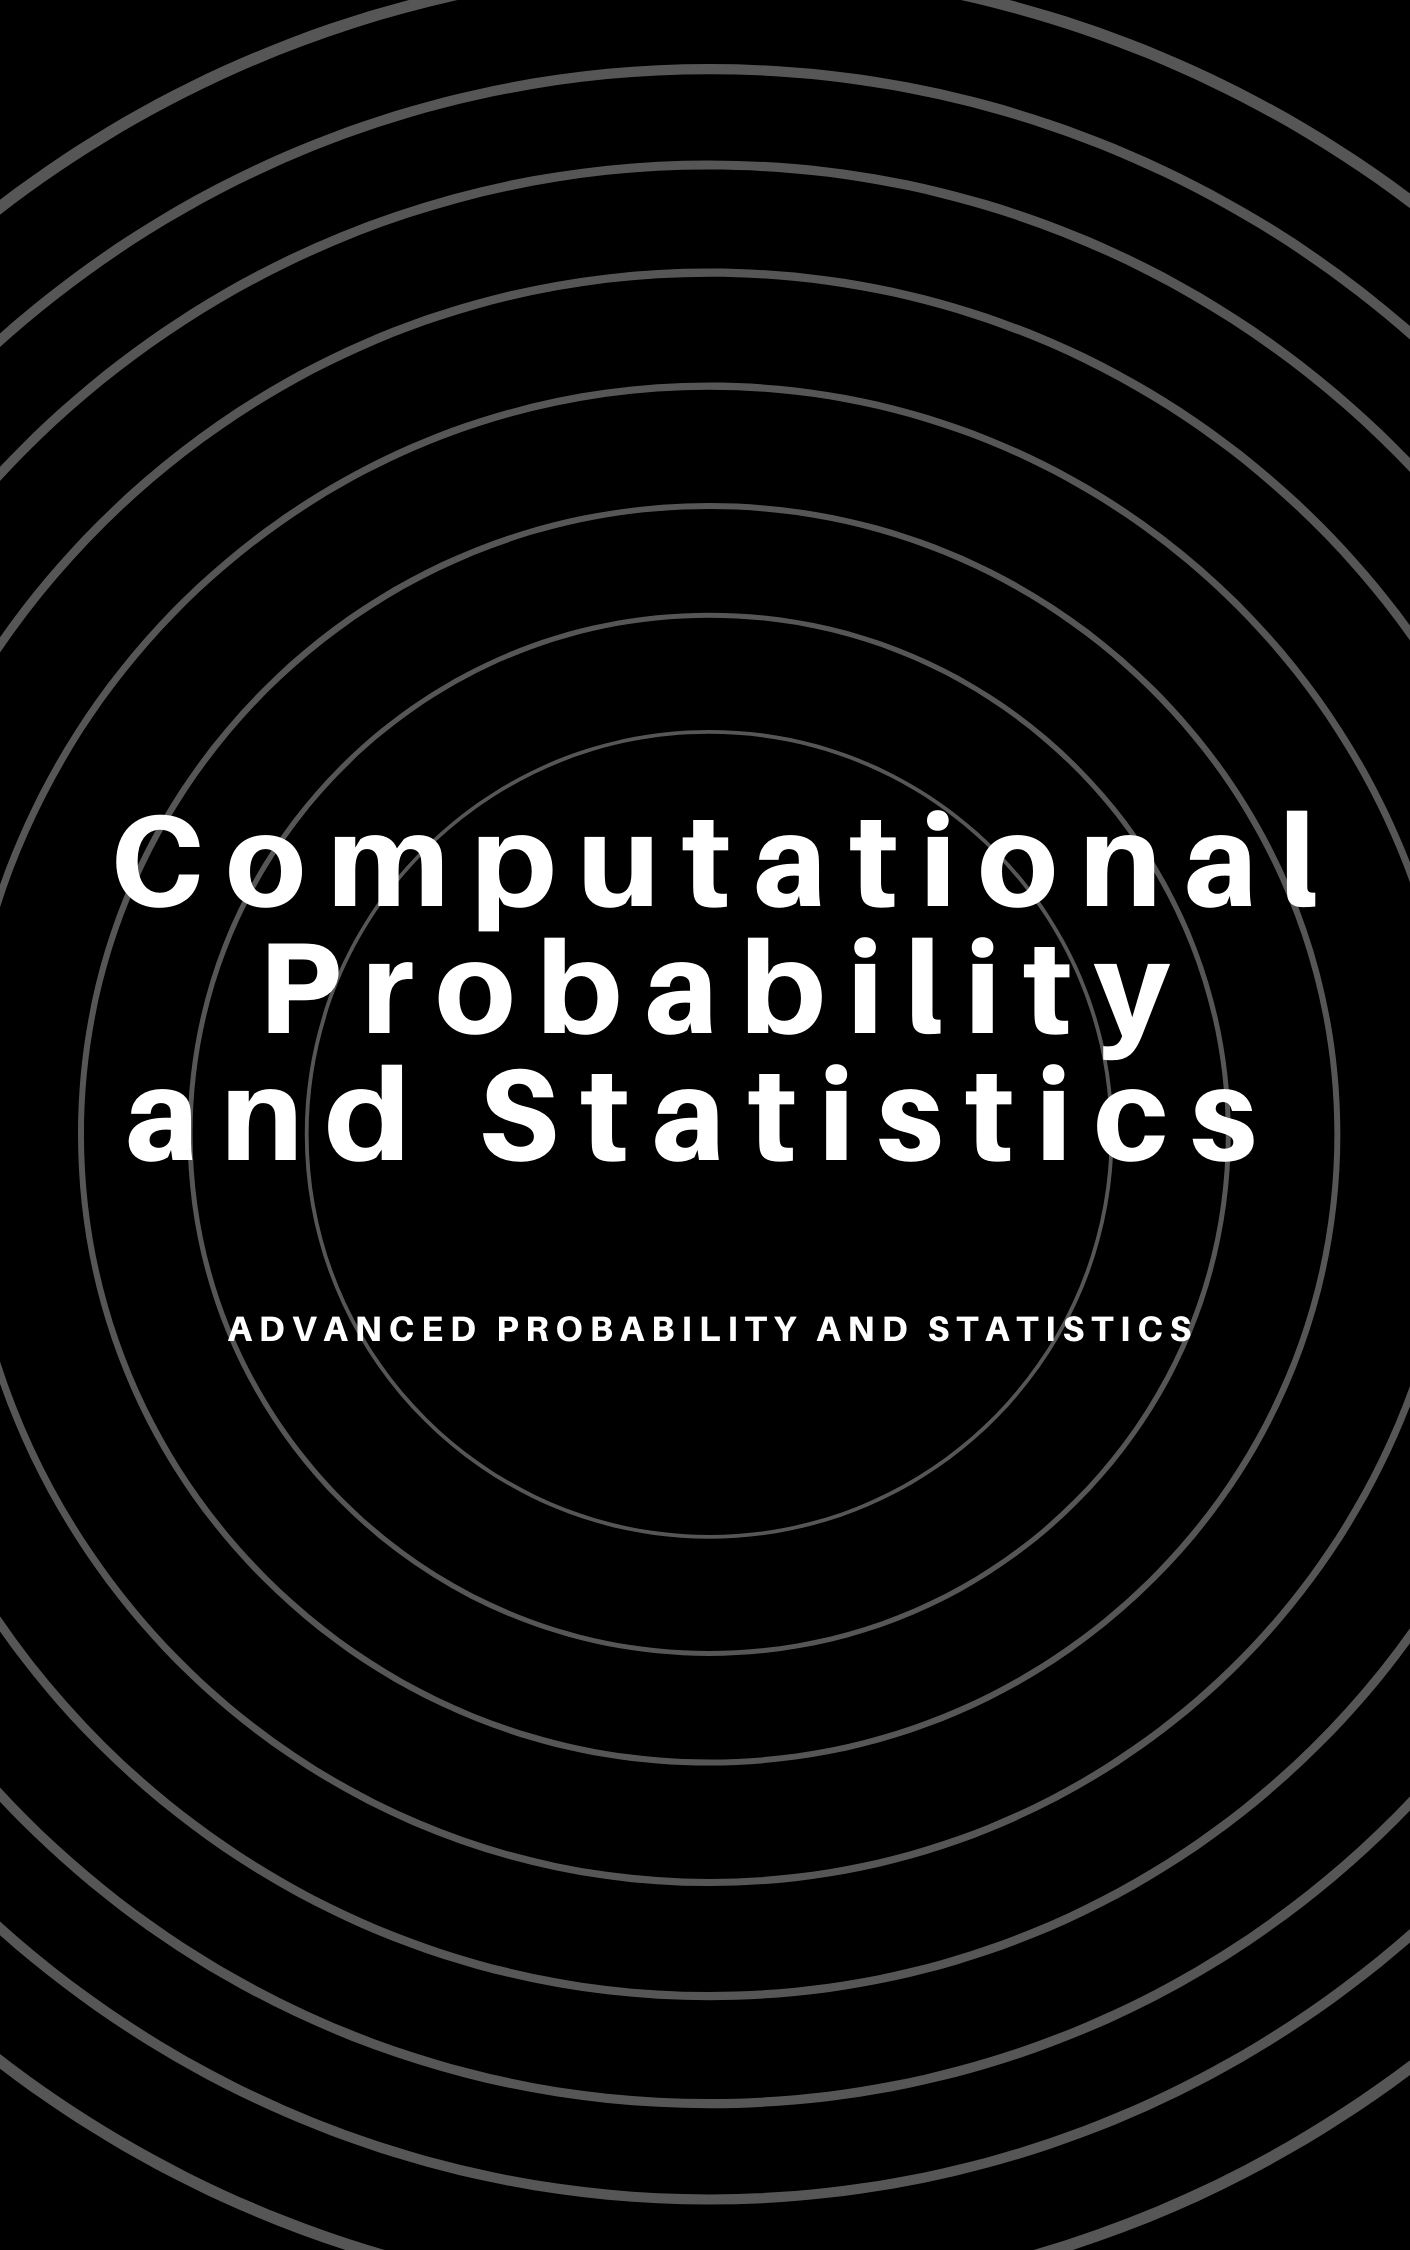
\includegraphics[width=19.58in]{./figures/Cover}

This book is based on the notes we created for our students as part of a one semester course on probability and statistics. We developed these notes from three primary resources. The most important is the Openintro Introductory Statistics with Randomization and Simulation \citep{ointrorand} book. In parts we have used their notes and homework problems. However, in most cases we have altered their work to fit our needs. The second most important book for our work is Introductory to Probability and Statistics with R \citep{ipsur}. Finally, we have used some examples, code, and ideas from the first addition of Prium's book Foundations and Applications of Statistics: An Introduction Using R \citep{pruim2011foundations}.

\hypertarget{who-is-this-book-for}{%
\section{Who is this book for?}\label{who-is-this-book-for}}

We designed this book for study of statistics that maximizes computational ideas while minimizing algebraic symbol manipulation. Although we do discuss traditional small sample normal based inference and some of the classical probability distributions, we rely heavily on ideas such as simulation, permutations, and bootstrap. This means that students with a background in differential and integral calculus will be successful with this book.

The book makes extensive using of the \texttt{R} programming language. In particular we focus both on the \textbf{tidyverse} and \textbf{mosaic} packages. We include a significant amount of code in our notes and frequently demonstrate multiple ways of completing a task. We have used this book for juniors and sophomores.

\hypertarget{book-structure-and-how-to-use-it}{%
\section{Book Structure and How to Use It}\label{book-structure-and-how-to-use-it}}

The book is divided into 4 parts. Each part starts with a case study that introduces many of the main ideas of each part. Each chapter is designed to be a standalone 50 minute lesson. Within each lesson, we give exercises that can be worked in class and we have learning objectives.

This book assumes students have access to \texttt{R}. Finally, we keep the number of homework problems to a reasonable level and assign all problems.

The four parts of the book are:

\begin{enumerate}
\def\labelenumi{\arabic{enumi}.}
\item
  Descriptive Statistical Modeling: This part introduces the student to data collection methods, summary statistics, visual summaries, and exploratory data analysis.
\item
  Probability: We discuss the foundation ideas of probability, counting methods, and common distributions. We use both calculus and simulation to find moments and probabilities. We introduce basic ideas of multivariate probability. We include method of moments and maximum likelihood estimators.
\item
  Statistical Inference: We discuss many of the basic inference ideas found in a traditional introductory statistics class but we add ideas of bootstrap and permutation methods.
\item
  Statistical Prediction: The final part introduces prediction methods mainly in the form of linear regression. This part does also include inference for regression.
\end{enumerate}

The learning outcomes for this course are to use computational and mathematical statistical/probabilistic concepts for:

\begin{enumerate}
\def\labelenumi{\alph{enumi}.}
\tightlist
\item
  Developing probabilistic models
\item
  Developing statistical models for description, inference, and prediction\\
\item
  Advancing practical and theoretical analytic experience and skills
\end{enumerate}

\hypertarget{prerequisites}{%
\section{Prerequisites}\label{prerequisites}}

To take this course, students are expected to have completed calculus up through and including integral calculus. We do have multivariate ideas in the course but they are easily taught and don't require calculus III. We don't assume the students have any programming experience and thus we include a great deal of code. We have historically supplemented the course with \href{http://datacamp.com/}{Data Camp} courses. We have also used \href{http://rstudio.cloud}{Rstudio Cloud} to help students get started without the burden of loading and maintaining software.

\hypertarget{packages}{%
\section{Packages}\label{packages}}

These notes make use of the following packages in R \textbf{knitr} \citep{R-knitr}, \textbf{rmarkdown} \citep{R-rmarkdown}, \textbf{mosaic} \citep{R-mosaic}, \textbf{mosaicCalc} \citep{R-mosaicCalc}, \textbf{tidyverse} \citep{R-tidyverse}, \textbf{ISLR} \citep{R-ISLR}, \textbf{vcd} \citep{R-vcd}, \textbf{ggplot2} \citep{R-ggplot2}, \textbf{MASS} \citep{R-MASS}, \textbf{openintro} \citep{R-openintro}, \textbf{broom} \citep{R-broom}, \textbf{infer} \citep{R-infer}, \textbf{ISLR} \citep{R-ISLR}, \textbf{kableExtra} \citep{R-kableExtra}, \textbf{DT} \citep{R-DT}.

\hypertarget{acknowledgements}{%
\section{Acknowledgements}\label{acknowledgements}}

We have been lucky to have numerous open sources to help facilitate this work.

This book was written using the \textbf{bookdown} package \citep{R-bookdown}.


\includegraphics[width=1.22in]{./figures/by-nc-sa}

This book is licensed under the \href{http://creativecommons.org/licenses/by-nc-sa/4.0/}{Creative Commons Attribution-NonCommercial-ShareAlike 4.0 International License}.

\hypertarget{file-creation-information}{%
\section{File Creation Information}\label{file-creation-information}}

\begin{itemize}
\tightlist
\item
  File creation date: 2021-07-26
\item
  R version 4.1.0 (2021-05-18)
\end{itemize}

\hypertarget{part-descriptive-statistical-modeling}{%
\part{Descriptive Statistical Modeling}\label{part-descriptive-statistical-modeling}}

\hypertarget{CS1}{%
\chapter{Case Study}\label{CS1}}

\hypertarget{objectives}{%
\section{Objectives}\label{objectives}}

\begin{enumerate}
\def\labelenumi{\arabic{enumi})}
\tightlist
\item
  Use R for basic analysis and visualization.\\
\item
  Compile a report using \texttt{knitr}.
\end{enumerate}

\hypertarget{introduction-to-descriptive-statistical-modeling}{%
\section{Introduction to Descriptive Statistical Modeling}\label{introduction-to-descriptive-statistical-modeling}}

In this first block of material we will focus on data types, collection methods, summaries, and visualizations. We also intend to introduce computing via the \texttt{R} package. Programming in \texttt{R} requires some focus early in the course and we will supplement with some online courses. There is relatively little mathematics in this first block.

\hypertarget{the-data-analytic-process}{%
\section{The data analytic process}\label{the-data-analytic-process}}

Scientists seek to answer questions using rigorous methods and careful observations. These observations -- collected from the likes of field notes, surveys, and experiments -- form the backbone of a statistical investigation and are called \textbf{data}. Statistics is the study of how best to collect, analyze, and draw conclusions from data. It is helpful to put statistics in the context of a general process of investigation:

\begin{enumerate}
\def\labelenumi{\arabic{enumi}.}
\item
  Identify a question or problem.
\item
  Collect relevant data on the topic.
\item
  Explore and understand the data.
\item
  Analyze the data.
\item
  Form a conclusion.
\item
  Make decisions based on the conclusion.
\end{enumerate}

This is typical of an explanatory process because it starts with a research question and proceeds. However, sometimes an analysis is exploratory. There is data but not necessarily a research question. The purpose of the analysis is to find interesting features in the data and sometimes generate hypotheses. In this course we focus on the explanatory aspects of analysis but we have examples of exploratory.

Statistics as a subject focuses on making stages 2-5 objective, rigorous, and efficient. That is, statistics has three primary components:

\begin{itemize}
\tightlist
\item
  How best can we collect data?\\
\item
  How should it be analyzed?\\
\item
  And what can we infer from the analysis?
\end{itemize}

The topics scientists investigate are as diverse as the questions they ask. However, many of these investigations can be addressed with a small number of data collection techniques, analytic tools, and fundamental concepts in statistical inference. This lesson provides a glimpse into these and other themes we will encounter throughout the rest of the course.

\hypertarget{case-study}{%
\section{Case study}\label{case-study}}

In this lesson we will consider an experiment that studies effectiveness of stents in treating patients at risk of stroke. \footnote{\href{http://www.nejm.org/doi/full/10.1056/NEJMoa1105335}{Chimowitz MI, Lynn MJ, Derdeyn CP, et al.~2011. Stenting versus Aggressive Medical Therapy for Intracranial Arterial Stenosis. New England Journal of Medicine 365:993-1003.}} \footnote{\href{http://www.nytimes.com/2011/09/08/health/research/08stent.html}{NY Times article reporting on the study}} Stents are small mesh tubes that are placed inside narrow or weak arteries to assist in patient recovery after cardiac events and reduce the risk of an additional heart attack or death. Many doctors have hoped that there would be similar benefits for patients at risk of stroke. We start by writing the principal question the researchers hope to answer:

\hypertarget{research-question}{%
\subsection{Research question}\label{research-question}}

\begin{quote}
Does the use of stents reduce the risk of stroke?
\end{quote}

\hypertarget{collect-the-relevant-data}{%
\subsection{Collect the relevant data}\label{collect-the-relevant-data}}

The researchers who asked this question collected data on 451 at-risk patients. Each volunteer patient was randomly assigned to one of two groups:

\textbf{Treatment group}. Patients in the treatment group received a stent and medical management. The medical management included medications, management of risk factors, and help in lifestyle modification.

\textbf{Control group}. Patients in the control group received the same medical management as the treatment group but did not receive stents.

Researchers randomly assigned 224 patients to the treatment group and 227 to the control group. In this study, the control group provides a reference point against which we can measure the medical impact of stents in the treatment group.

This is an experiment and not an observational study. We will learn more about these ideas in this block.

Researchers studied the effect of stents at two time points: 30 days after enrollment and 365 days after enrollment.

\hypertarget{import-data}{%
\subsection{Import data}\label{import-data}}

We begin our first use of \texttt{R}

If you need to install a package, most likely it will be on CRAN, the Comprehensive R Archive Network. Before
a package can be used, it must be installed on the computer (once per computer or account) and loaded into a session (once per \texttt{R} session). When you exit \texttt{R}, the package stays installed on the computer but will not be reloaded when \texttt{R} is started again.

In summary, \texttt{R} has packages that can be downloaded and installed from online repositories such as CRAN. When you install a package, which only needs to be done once per computer or account, in \texttt{R} all it is doing is placing the source code in a library folder designated during the installation of \texttt{R}. Packages are typically collections of functions and variables that are specific to a certain task or subject matter.

For example, to install the mosaic package, enter:

\begin{verbatim}
install.packages("mosaic") # fetch package from CRAN
\end{verbatim}

In RStudio there is a \emph{Packages} tab that makes it easy to add and maintain packages.

To use a package in a session, we must load it which makes it available to the current session only. When you start \texttt{R} again, you will have to load packages again. The command \texttt{library()} with the package name supplied as the argument is all that is needed. For this session, we will load \texttt{tidyverse} and \texttt{mosaic}. Note: the box below is executing the \texttt{R} commands, this is known as reproducible research since you can see the code and then you can run or modify as you need.

\begin{Shaded}
\begin{Highlighting}[]
\FunctionTok{library}\NormalTok{(tidyverse)}
\FunctionTok{library}\NormalTok{(mosaic)}
\end{Highlighting}
\end{Shaded}

Next read in the data into the working environment.

\begin{Shaded}
\begin{Highlighting}[]
\NormalTok{stent\_study }\OtherTok{\textless{}{-}} \FunctionTok{read\_csv}\NormalTok{(}\StringTok{"data/stent\_study.csv"}\NormalTok{)}
\end{Highlighting}
\end{Shaded}

Let's break this code down. We are reading from a .csv file and assigning the results into an object called \texttt{stent\_study}. The assignment arrow \texttt{\textless{}-} means we assign what is on the right to what is on the left. The \texttt{R} function we use in this case is \texttt{read\_csv()}; when using \texttt{R} functions, you should ask yourself:

\begin{enumerate}
\def\labelenumi{\arabic{enumi}.}
\item
  What do I want \texttt{R} to do?
\item
  What information must I provide for \texttt{R} to do this?
\end{enumerate}

We want \texttt{R} to read in a .csv file. We can get help on this function by typing \texttt{?read\_csv} at the prompt. The only required input to \texttt{read\_csv()} is the file location. We have our data stored in a folder called ``data'' under the working directory. We can determine the working directory by typing \texttt{getwd()} at the prompt.

\begin{Shaded}
\begin{Highlighting}[]
\FunctionTok{getwd}\NormalTok{()}
\end{Highlighting}
\end{Shaded}

Similarly, if we wish to change the working directory, we can do so by using the \texttt{setwd()} function:

\begin{Shaded}
\begin{Highlighting}[]
\FunctionTok{setwd}\NormalTok{(}\StringTok{\textquotesingle{}C:/Users/Brad.Warner/Documents/Classes/Math 377/Another Folder\textquotesingle{}}\NormalTok{)}
\end{Highlighting}
\end{Shaded}

In \texttt{R} if you use the \texttt{view()}, you will see the data in what looks like a standard spreadsheet.

\begin{Shaded}
\begin{Highlighting}[]
\FunctionTok{view}\NormalTok{(stent\_study)}
\end{Highlighting}
\end{Shaded}

\hypertarget{explore-data}{%
\subsection{Explore data}\label{explore-data}}

Before we attempt to answer the research question, let's look at the data. We want \texttt{R} to print out the first 10 rows of the data. The appropriate function is \texttt{head()} and it needs the data object. By default, \texttt{R} will output the first 6 rows. By using the \texttt{n=} argument, we can specify how many rows we want to view.

\begin{Shaded}
\begin{Highlighting}[]
\FunctionTok{head}\NormalTok{(stent\_study,}\AttributeTok{n=}\DecValTok{10}\NormalTok{)}
\end{Highlighting}
\end{Shaded}

\begin{verbatim}
## # A tibble: 10 x 3
##    group   outcome30 outcome365
##    <chr>   <chr>     <chr>     
##  1 control no_event  no_event  
##  2 trmt    no_event  no_event  
##  3 control no_event  no_event  
##  4 trmt    no_event  no_event  
##  5 trmt    no_event  no_event  
##  6 control no_event  no_event  
##  7 trmt    no_event  no_event  
##  8 control no_event  no_event  
##  9 control no_event  no_event  
## 10 control no_event  no_event
\end{verbatim}

We also want to ``inspect'' the data. The function is \texttt{inspect()} and \texttt{R} needs the data object \texttt{stent\_study}.

\begin{Shaded}
\begin{Highlighting}[]
\FunctionTok{inspect}\NormalTok{(stent\_study)}
\end{Highlighting}
\end{Shaded}

\begin{verbatim}
## 
## categorical variables:  
##         name     class levels   n missing
## 1      group character      2 451       0
## 2  outcome30 character      2 451       0
## 3 outcome365 character      2 451       0
##                                    distribution
## 1 control (50.3%), trmt (49.7%)                
## 2 no_event (89.8%), stroke (10.2%)             
## 3 no_event (83.8%), stroke (16.2%)
\end{verbatim}

To keep things simple we will only look at the \texttt{outcome30} variable in this case study. We will summarize the data in a table. Later in the course, we will learn to do this using the \texttt{tidy} package; for now we use the \texttt{mosaic} package. This package makes use of the modeling formula that you will use extensively later in this course and in Math 378.

We want to summarize the data by making a table. In \texttt{mosaic} this is the \texttt{tally()} function. Before using this function, we have to understand the basic formula notation that \texttt{mosaic} uses. The basic format is:

\begin{verbatim}
goal( y ~ x, data = MyData, ... ) # pseudo-code for the formula template
\end{verbatim}

We read \texttt{y\ \textasciitilde{}\ x} as ``y tilde x'' and interpret it in the equivalent forms: ``y broken down by x''; ``y modeled by x''; ``y explained by x''; ``y depends on x''; or ``y accounted for by x.'' For graphics, it's reasonable to read the formula as ``y vs.~x'', which is exactly the convention used for coordinate axes.

For this exercise, we want to apply \texttt{tally()} to the variables \texttt{group} and \texttt{outcome30}. In this case it does not matter which we call \texttt{y} and \texttt{x}; however, it is more natural to think of \texttt{outcome30} as a dependent variable.

\begin{Shaded}
\begin{Highlighting}[]
\FunctionTok{tally}\NormalTok{(outcome30}\SpecialCharTok{\textasciitilde{}}\NormalTok{group,}\AttributeTok{data=}\NormalTok{stent\_study,}\AttributeTok{margins =} \ConstantTok{TRUE}\NormalTok{)}
\end{Highlighting}
\end{Shaded}

\begin{verbatim}
##           group
## outcome30  control trmt
##   no_event     214  191
##   stroke        13   33
##   Total        227  224
\end{verbatim}

The \texttt{margins} option totals the columns.

Of the 224 patients in the treatment group, 33 had a stroke by the end of the first month. Using these two numbers, we can use \texttt{R} to compute the proportion of patients in the treatment group who had a stroke by the end of their first month.

\begin{Shaded}
\begin{Highlighting}[]
\DecValTok{33}\SpecialCharTok{/}\NormalTok{(}\DecValTok{33}\SpecialCharTok{+}\DecValTok{191}\NormalTok{)}
\end{Highlighting}
\end{Shaded}

\begin{verbatim}
## [1] 0.1473214
\end{verbatim}

\begin{quote}
\textbf{Exercise}:\\
What proportion of the control group had a stroke? And why is this answer different from what \texttt{inspect()} reports?
\end{quote}

Let's have \texttt{R} calculate proportions for us. Use \texttt{?} to look at the help menu for \texttt{tally()}. Note that one of the option arguments of the \texttt{tally()} function is \texttt{format=}. Setting this equal to \texttt{proportion} will output the proportions instead of the counts.

\begin{Shaded}
\begin{Highlighting}[]
\FunctionTok{tally}\NormalTok{(outcome30}\SpecialCharTok{\textasciitilde{}}\NormalTok{group,}\AttributeTok{data=}\NormalTok{stent\_study,}\AttributeTok{format=}\StringTok{\textquotesingle{}proportion\textquotesingle{}}\NormalTok{,}\AttributeTok{margins =} \ConstantTok{TRUE}\NormalTok{)}
\end{Highlighting}
\end{Shaded}

\begin{verbatim}
##           group
## outcome30     control       trmt
##   no_event 0.94273128 0.85267857
##   stroke   0.05726872 0.14732143
##   Total    1.00000000 1.00000000
\end{verbatim}

We can compute summary statistics from the table. A \textbf{summary statistic} is a single number summarizing a large amount of data.\footnote{Formally, a summary statistic is a value computed from the data. Some summary statistics are more useful than others.} For instance, the primary results of the study after 1 month could be described by two summary statistics: the proportion of people who had a stroke in the treatment and control groups.

\begin{itemize}
\item
  Proportion who had a stroke in the treatment (stent) group: \(33/224 = 0.15 = 15\%\).
\item
  Proportion who had a stroke in the control group: \(13/227 = 0.06 = 6\%\).
\end{itemize}

\hypertarget{visualize-the-data}{%
\subsection{Visualize the data}\label{visualize-the-data}}

It is often important to visualize the data. The table is a type of visualization but in this section we will introduce a graphical method called bar charts.

We will use the \href{https://cran.r-project.org/web/packages/ggformula/vignettes/ggformula-blog.html}{\textbf{ggformula}} package to visualize. It is a wrapper to the \texttt{ggplot2} package which is becoming the industry standard for generating professional graphics. However, its interface is difficult to learn and we will ease into by using \texttt{ggformula} which makes use of the formula notation introduced above. The \textbf{ggformula} package was loaded when we loaded \textbf{mosaic}.\footnote{\url{https://cran.r-project.org/web/packages/ggformula/vignettes/ggformula-blog.html}}

To generate a basic graphic, we need to ask ourselves what information we are trying to see, what particular type of graph is best, what corresponding \texttt{R} function to use, and what information that \texttt{R} function needs in order to build a plot. For categorical data we want a bar chart and the \texttt{R} function \texttt{gf\_bar()} needs the data object and the variable(s) of interest.

Here is our first attempt. In Figure \ref{fig:first-fig}, we leave the \texttt{y} portion of our formula blank. Doing this implies that we simply want to view the number/count of \texttt{outcome30} by type. We will see the two levels of \texttt{outcome30} on the x-axis and counts on the y-axis.



\begin{Shaded}
\begin{Highlighting}[]
\FunctionTok{gf\_bar}\NormalTok{(}\SpecialCharTok{\textasciitilde{}}\NormalTok{outcome30,}\AttributeTok{data=}\NormalTok{stent\_study)}
\end{Highlighting}
\end{Shaded}

\begin{figure}
\centering
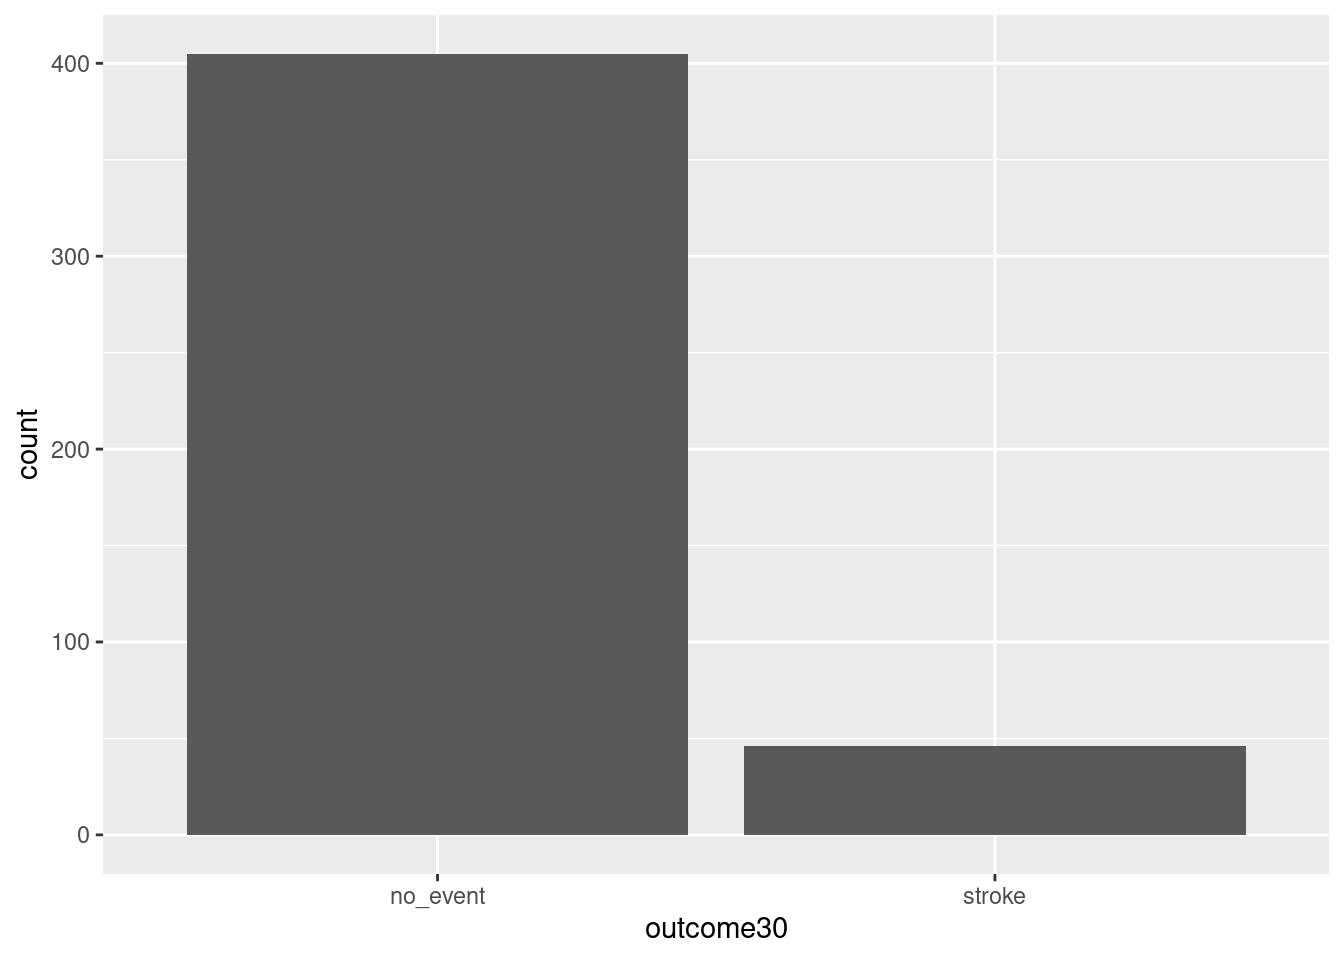
\includegraphics{01-Data-Case-Study_files/figure-latex/first-fig-1.pdf}
\caption{\label{fig:first-fig}Using \textbf{ggformula} to create a bar chart.}
\end{figure}

\begin{quote}
\textbf{Exercise}:\\
Explain Figure \ref{fig:first-fig}..
\end{quote}

This plot graphically shows us the total number of ``stroke'' and the total number of ``no\_event''. However, this is not what we want. We want to compare the 30-day outcomes for both treatment groups. So we need to break the data into different groups based on treatment type. In the formula language we now update it to the form:

\begin{verbatim}
goal( y ~ x|z, data = MyData, ... ) # pseudo-code for the formula template
\end{verbatim}

We read \texttt{y\ \textasciitilde{}\ x\textbar{}z} as ``y tilde x by z'' and interpret in the equivalent forms: ``y modeled by x for each z''; ``y explained by x within each z''; or ``y accounted for by x within z.'' For graphics, it's reasonable to read the formula as ``y vs.~x for each z''. Figure \ref{fig:split-fig} shows the results.



\begin{Shaded}
\begin{Highlighting}[]
\FunctionTok{gf\_bar}\NormalTok{(}\SpecialCharTok{\textasciitilde{}}\NormalTok{outcome30}\SpecialCharTok{|}\NormalTok{group,}\AttributeTok{data =}\NormalTok{ stent\_study) }
\end{Highlighting}
\end{Shaded}

\begin{figure}
\centering
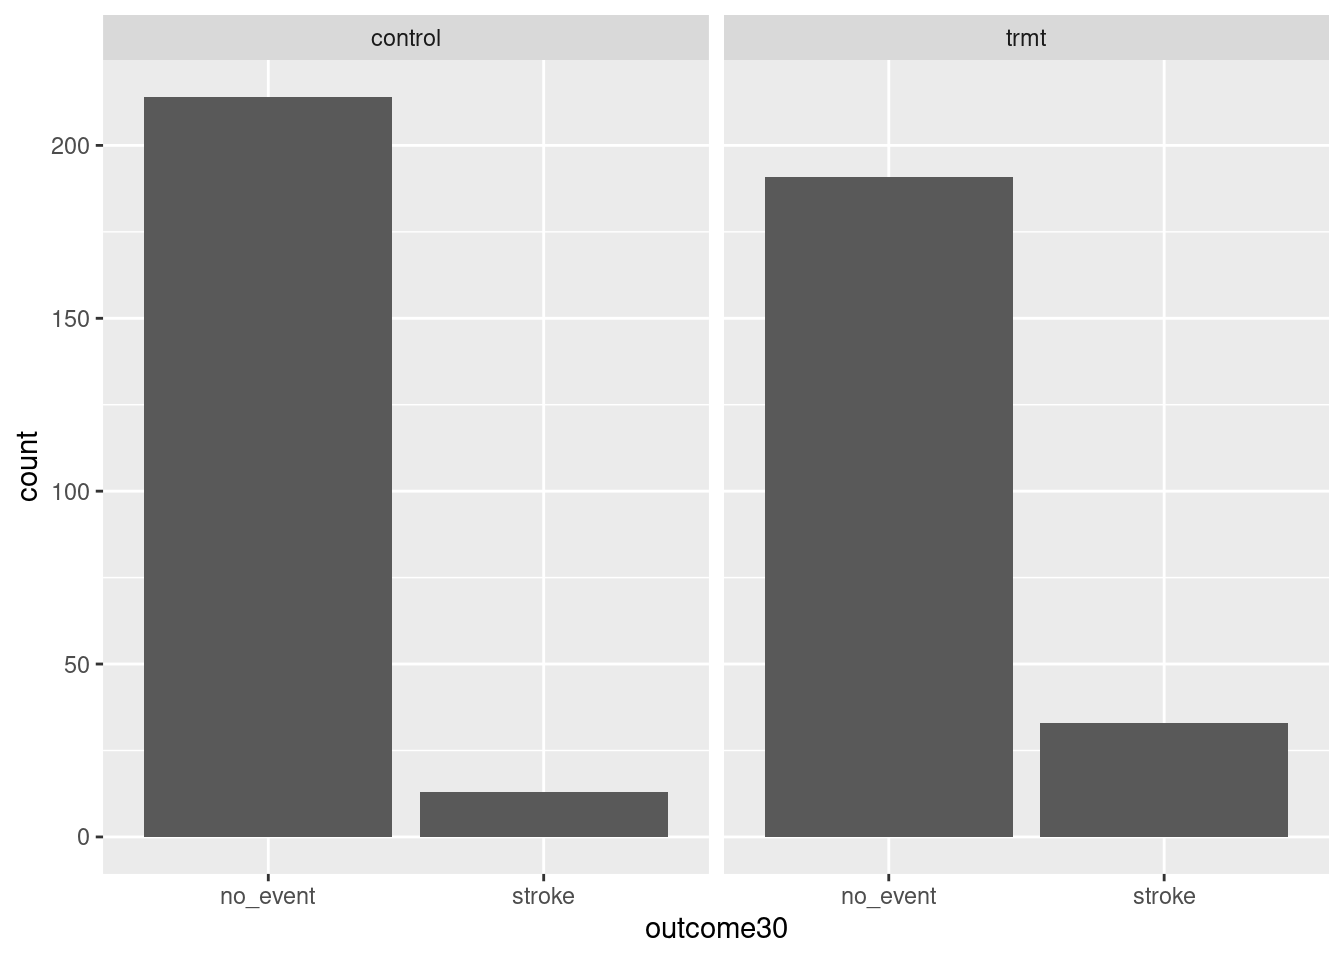
\includegraphics{01-Data-Case-Study_files/figure-latex/split-fig-1.pdf}
\caption{\label{fig:split-fig}Bar charts conditioned on the \texttt{group} variable.}
\end{figure}

\hypertarget{more-advanced-graphics}{%
\subsubsection{More advanced graphics}\label{more-advanced-graphics}}

As a prelude for things to come, the above graphic needs work. The labels don't help; there is no title; we could add color; does it make more sense to use proportions? Here is the code and results for a better graph, see Figure \ref{fig:cs1-fig}.. Don't worry if this seems a bit advanced, but feel free to examine each new component of this code.

\begin{Shaded}
\begin{Highlighting}[]
\NormalTok{stent\_study }\SpecialCharTok{\%\textgreater{}\%}
\FunctionTok{gf\_props}\NormalTok{(}\SpecialCharTok{\textasciitilde{}}\NormalTok{group,}\AttributeTok{fill=}\SpecialCharTok{\textasciitilde{}}\NormalTok{outcome30,}\AttributeTok{position=}\StringTok{\textquotesingle{}fill\textquotesingle{}}\NormalTok{) }\SpecialCharTok{\%\textgreater{}\%}
  \FunctionTok{gf\_labs}\NormalTok{(}\AttributeTok{title=}\StringTok{"Impact of Stents of Stroke"}\NormalTok{,}
          \AttributeTok{subtitle=}\StringTok{\textquotesingle{}Experiment with 451 Patients\textquotesingle{}}\NormalTok{,}
          \AttributeTok{x=}\StringTok{"Experimental Group"}\NormalTok{,}
          \AttributeTok{y=}\StringTok{"Number of Events"}\NormalTok{) }\SpecialCharTok{\%\textgreater{}\%}
  \FunctionTok{gf\_theme}\NormalTok{(}\FunctionTok{theme\_bw}\NormalTok{())}
\end{Highlighting}
\end{Shaded}

\begin{figure}
\centering
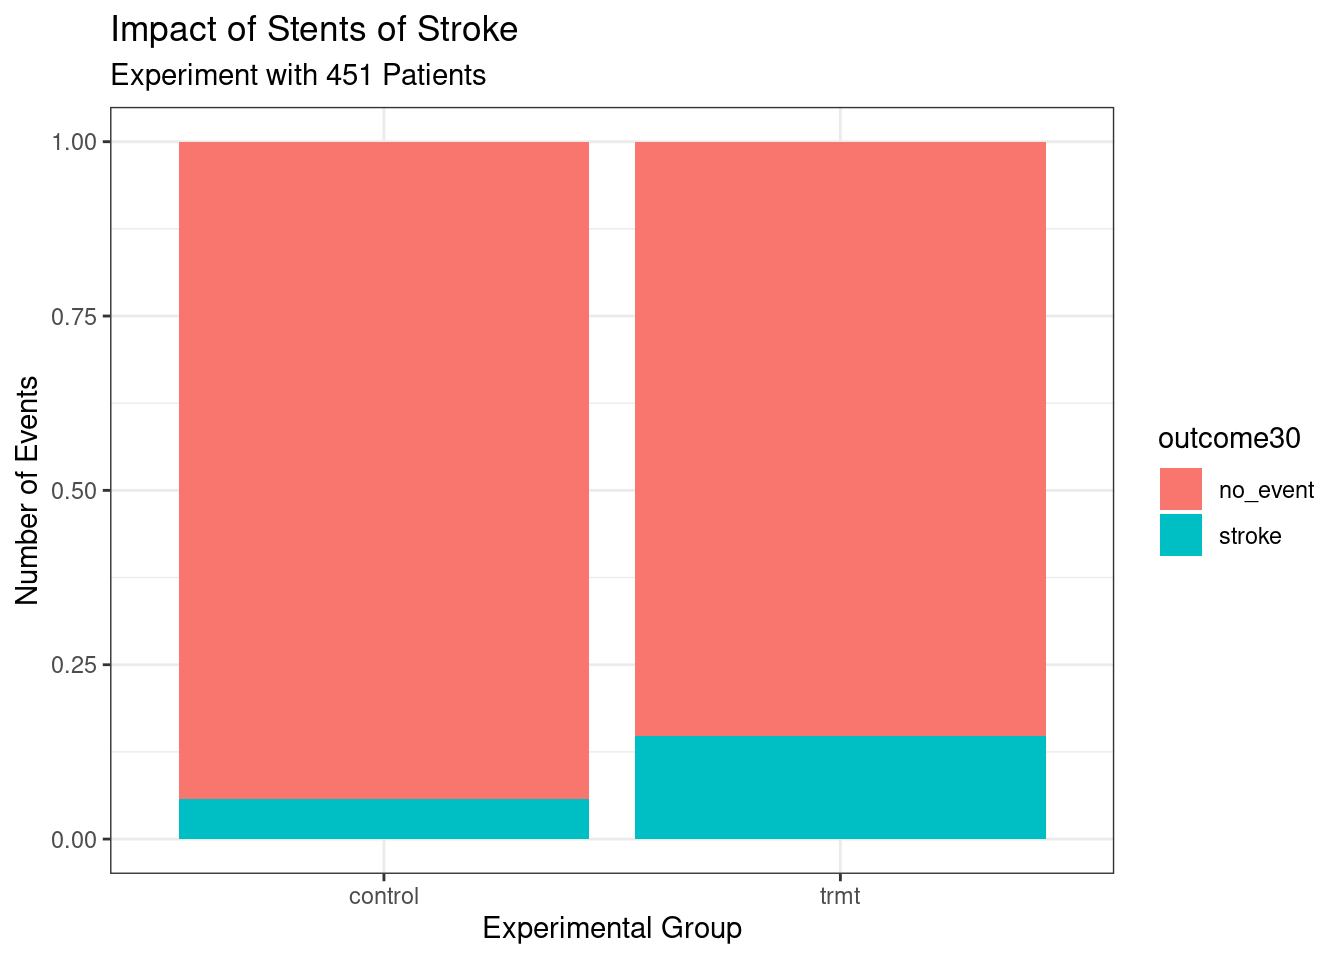
\includegraphics{01-Data-Case-Study_files/figure-latex/cs1-fig-1.pdf}
\caption{\label{fig:cs1-fig}Better graph.}
\end{figure}

Notice that we used the pipe operator, \texttt{\%\textgreater{}\%}. This operator allows us to string functions together in a manner that makes it easier to read the code. In the above code we are sending the data object \texttt{stent\_study} into the function \texttt{gf\_props()} to use as data so we don't need the \texttt{data\ =} argument. In math, this is a composition of functions. Instead of \texttt{f(g(x))} we could use a pipe \texttt{f(g(x))\ =\ g(x)\ \%\textgreater{}\%\ f()}.

\hypertarget{conclusion}{%
\subsection{Conclusion}\label{conclusion}}

These two summary statistics are useful in looking for differences in the groups, and we are in for a surprise: an additional 9\% of patients in the treatment group had a stroke! This is important for two reasons. First, it is contrary to what doctors expected, which was that stents would \emph{reduce} the rate of strokes. Second, it leads to a statistical question: do the data show a \textbf{real} difference due to the treatment?

This second question is subtle. Suppose you flip a coin 100 times. While the chance a coin lands heads in any given coin flip is 50\%, we probably won't observe exactly 50 heads. This type of fluctuation is part of almost any type of data generating process. It is possible that the 9\% difference in the stent study is due to this natural variation. However, the larger the difference we observe (for a particular sample size), the less believable it is that the difference is due to chance. So what we are really asking is the following: is the difference so large that we should reject the notion that it was due to chance?

This is a preview of step 4, analyze the data, and step 5, form a conclusion, of the analysis cycle. While we haven't yet covered statistical tools to fully address these steps, we can comprehend the conclusions of the published analysis: there was compelling evidence of harm by stents in this study of stroke patients.

\textbf{Be careful:} do not generalize the results of this study to all patients and all stents. This study looked at patients with very specific characteristics who volunteered to be a part of this study and who may not be representative of all stroke patients. In addition, there are many types of stents and this study only considered the self-expanding Wingspan stent (Boston Scientific). However, this study does leave us with an important lesson: we should keep our eyes open for surprises.

\hypertarget{homework-problems}{%
\section{Homework Problems}\label{homework-problems}}

Create an Rmd file \texttt{01\ Data\ Case\ Study\ Application.Rmd} in R, it may be provided, and start by inserting your name in the header. Code blocks below can be inserted and then you can complete the code and answer the questions. When you are done, \texttt{knit} it into a pdf file.

To create an \texttt{R} code chunk, use CTRL-ALT-I or on the \texttt{insert} tab of the window, use the drop down to select \texttt{R}. Anything between the dashes is interpreted as \texttt{R} code.

For more on RMarkdown see the video, \url{https://www.youtube.com/watch?v=DNS7i2m4sB0} This video assumes you are using \texttt{R} on your computer but we are using RStudio Cloud. Thus we can \texttt{knit} to a pdf since it is setup for us. You can also take the first chapter of the Data Camp course Reporting with R Markdown to learn more.

\begin{enumerate}
\def\labelenumi{\arabic{enumi}.}
\tightlist
\item
  \textbf{Stent study continued}. Complete a similar analysis for the stent data but this time for the one year data. In particular
\end{enumerate}

\begin{enumerate}
\def\labelenumi{\alph{enumi}.}
\tightlist
\item
  Read the data into your working directory.
\end{enumerate}

\begin{verbatim}
stent_study <-read_csv(___)
\end{verbatim}

\begin{enumerate}
\def\labelenumi{\alph{enumi}.}
\setcounter{enumi}{1}
\tightlist
\item
  Complete similar steps as in the class notes. The start of code is provided below.
  i. Use \texttt{inspect} on the data.\\
  ii. Create a table of \texttt{outcome365} and \texttt{group}. Comment on the results.\\
  iii. Create a barchart of the data.
\end{enumerate}

Summary

\begin{verbatim}
inspect(___)
\end{verbatim}

Table

\begin{verbatim}
tally(outcome365~___,data=stent_study,format=___,margins = TRUE)
\end{verbatim}

Barchart

\begin{verbatim}
stent_study %>%
  gf_props(~___,fill=~___,position='fill') %>%
  gf_labs(title=___
  subtitle=___,
  x=___,
  y=___)
\end{verbatim}

\begin{enumerate}
\def\labelenumi{\arabic{enumi}.}
\setcounter{enumi}{1}
\tightlist
\item
  \textbf{Migraine and acupuncture}. A migraine is a particularly painful type of headache, which patients sometimes wish to treat with acupuncture. To determine whether acupuncture relieves migraine pain, researchers conducted a randomized controlled study where 89 females diagnosed with migraine headaches were randomly assigned to one of two groups: treatment or control. 43 patients in the treatment group received acupuncture that is specifically designed to treat migraines. 46 patients in the control group received placebo acupuncture (needle insertion at nonacupoint locations). 24 hours after patients received acupuncture, they were asked if they were pain free.\footnote{G. Allais et al.~\href{http://www.ncbi.nlm.nih.gov/pubmed/21533739}{``Ear acupuncture in the treatment of migraine attacks: a randomized trial on the efficacy of appropriate versus inappropriate acupoints''.} In: Neurological Sci. 32.1 (2011), pp.~173--175.}
\end{enumerate}

The data is in the file \texttt{migraine\_study.csv} in the folder \texttt{data}.

Complete the following work:

\begin{enumerate}
\def\labelenumi{\alph{enumi}.}
\tightlist
\item
  Read the data an object called \texttt{migraine\_study}.
\end{enumerate}

\begin{verbatim}
migraine_study <- read_csv("data/___")
\end{verbatim}

\begin{verbatim}
head(migraine_study)
\end{verbatim}

\begin{enumerate}
\def\labelenumi{\alph{enumi}.}
\setcounter{enumi}{1}
\tightlist
\item
  Create a table of the data.
\end{enumerate}

\begin{verbatim}
tally(___)
\end{verbatim}

\begin{enumerate}
\def\labelenumi{\alph{enumi}.}
\setcounter{enumi}{2}
\tightlist
\item
  Report the percent of patients in the treatment group who were pain free 24 hours after receiving acupuncture.\\
\item
  Repeat for the control group.\\
\item
  At first glance, does acupuncture appear to be an effective treatment for migraines? Explain your reasoning.\\
\item
  Do the data provide convincing evidence that there is a real pain reduction for those patients in the treatment group? Or do you think that the observed difference might just be due to chance?
\end{enumerate}

Compile, \texttt{knit}, this report into a pdf.

\hypertarget{DB}{%
\chapter{Data Basics}\label{DB}}

\hypertarget{objectives-1}{%
\section{Objectives}\label{objectives-1}}

\begin{enumerate}
\def\labelenumi{\arabic{enumi})}
\tightlist
\item
  Define and use properly in context all new terminology to include but not limited to case, observational unit, variables, data frame, associated variables, independent, and discrete and continuous variables.\\
\item
  Identify and define the different types of variables.\\
\item
  From reading a study, explain the research question.\\
\item
  Create a scatterplot in \texttt{R} and determine the association of two numerical variables from the plot.
\end{enumerate}

\hypertarget{data-basics}{%
\section{Data basics}\label{data-basics}}

Effective presentation and description of data is a first step in most analyses. This lesson introduces one structure for organizing data as well as some terminology that will be used throughout this course.

\hypertarget{observations-variables-and-data-matrices}{%
\subsection{Observations, variables, and data matrices}\label{observations-variables-and-data-matrices}}

For reference we will be using a data set concerning 50 emails received in 2012. These observations will be referred to as the \texttt{email50} data set, and they are a random sample from a larger data set. This data is in the \textbf{openintro} package so let's load our packages.

\begin{Shaded}
\begin{Highlighting}[]
\FunctionTok{library}\NormalTok{(usdata)}
\end{Highlighting}
\end{Shaded}

Table \ref{tab:db1-tab} shows 5 rows of the \texttt{email50} data set concerning 50 emails from 2012. The data object \texttt{email50} is a subset of \texttt{email} and we have selected to only list 5 rows and 5 variables for ease of observation.

Each row in the table represents a single email or \textbf{case}.\footnote{A case is also sometimes called a \textbf{unit of observation} or an \textbf{observational unit}} The columns represent characteristics, called \textbf{variables}, for each of the emails. For example, the first row represents email 1, which is not spam, contains 21,705 characters, 551 line breaks, is written in HTML format, and contains only small numbers.

\label{tab:db1-tab}First 5 rows of email data frame

spam

num\_char

line\_breaks

format

number

0

21.705

551

1

small

0

7.011

183

1

big

1

0.631

28

0

none

0

15.829

242

1

small

Let's look at the first 10 rows of data from \texttt{email50} using \texttt{R}. Remember to ask the two questions:

\emph{What do we want \texttt{R} to do?} and

\emph{What must we give \texttt{R} for it to do this?}

We want the first 10 rows so we use \texttt{head} and \texttt{R} needs the data object and the number of rows. The data object is called \texttt{email50} and is accessible once the \textbf{openintro} package is loaded.

\begin{Shaded}
\begin{Highlighting}[]
\FunctionTok{head}\NormalTok{(email50,}\AttributeTok{n=}\DecValTok{10}\NormalTok{)}
\end{Highlighting}
\end{Shaded}

\begin{verbatim}
## # A tibble: 10 x 21
##    spam  to_multiple from     cc sent_email time                image attach
##    <fct> <fct>       <fct> <int> <fct>      <dttm>              <dbl>  <dbl>
##  1 0     0           1         0 1          2012-01-04 13:19:16     0      0
##  2 0     0           1         0 0          2012-02-16 20:10:06     0      0
##  3 1     0           1         4 0          2012-01-04 15:36:23     0      2
##  4 0     0           1         0 0          2012-01-04 17:49:52     0      0
##  5 0     0           1         0 0          2012-01-27 09:34:45     0      0
##  6 0     0           1         0 0          2012-01-17 17:31:57     0      0
##  7 0     0           1         0 0          2012-03-18 04:18:55     0      0
##  8 0     0           1         0 1          2012-03-31 13:58:56     0      0
##  9 0     0           1         1 1          2012-01-11 01:57:54     0      0
## 10 0     0           1         0 0          2012-01-07 19:29:16     0      0
## # ... with 13 more variables: dollar <dbl>, winner <fct>, inherit <dbl>,
## #   viagra <dbl>, password <dbl>, num_char <dbl>, line_breaks <int>,
## #   format <fct>, re_subj <fct>, exclaim_subj <dbl>, urgent_subj <fct>,
## #   exclaim_mess <dbl>, number <fct>
\end{verbatim}

In practice, it is especially important to ask clarifying questions to ensure important aspects of the data are understood. For instance, it is always important to be sure we know what each variable means and the units of measurement. Descriptions of all variables in the \texttt{email50} data set are given in its documentation which can be accessed in \texttt{R} by using the \texttt{?} command:

\begin{verbatim}
?email50
\end{verbatim}

(Note that not all data sets will have associated documentation; the authors of \textbf{openintro} package included this documentation with the \texttt{email50} data set contained in the package.)

The data in \texttt{email50} represent a \textbf{data matrix} or in \texttt{R} terminology \textbf{data frame} or \textbf{tibble} \footnote{A tibble is a data frame with attributes for such things as better display and printing}, which is a common way to organize data. Each row of a data matrix corresponds to a unique case, and each column corresponds to a variable. This is called \textbf{tidy data}.\footnote{For more information on tidy data see the \href{https://simplystatistics.org/2016/02/17/non-tidy-data/}{blog} and the \href{https://r4ds.had.co.nz/tidy-data.html\#pivoting}{book}.} The data frame for the stroke study introduced in the previous lesson had patients as the cases and there were three variables recorded for each patient. If we are thinking of patients as the unit of observation, then this data is tidy.

\begin{verbatim}
## # A tibble: 10 x 3
##    group   outcome30 outcome365
##    <chr>   <chr>     <chr>     
##  1 control no_event  no_event  
##  2 trmt    no_event  no_event  
##  3 control no_event  no_event  
##  4 trmt    no_event  no_event  
##  5 trmt    no_event  no_event  
##  6 control no_event  no_event  
##  7 trmt    no_event  no_event  
##  8 control no_event  no_event  
##  9 control no_event  no_event  
## 10 control no_event  no_event
\end{verbatim}

If we think of an outcome as a unit of observation then it is not tidy since the two outcome columns are variable values (month or year). The tidy data for this case would be:

\begin{verbatim}
## # A tibble: 10 x 4
##    patient_id group   time  result  
##         <int> <chr>   <chr> <chr>   
##  1          1 control month no_event
##  2          1 control year  no_event
##  3          2 trmt    month no_event
##  4          2 trmt    year  no_event
##  5          3 control month no_event
##  6          3 control year  no_event
##  7          4 trmt    month no_event
##  8          4 trmt    year  no_event
##  9          5 trmt    month no_event
## 10          5 trmt    year  no_event
\end{verbatim}

There are three interrelated rules which make a data set tidy:

\begin{enumerate}
\def\labelenumi{\arabic{enumi}.}
\tightlist
\item
  Each variable must have its own column.\\
\item
  Each observation must have its own row.\\
\item
  Each value must have its own cell.
\end{enumerate}

Why ensure that your data is tidy? There are two main advantages:

\begin{enumerate}
\def\labelenumi{\arabic{enumi}.}
\item
  There's a general advantage to picking one consistent way of storing data. If you have a consistent data structure, it's easier to learn the tools that work with it because they have an underlying uniformity.
\item
  There's a specific advantage to placing variables in columns because it allows \texttt{R}'s vectorised nature to shine. This will be more clear as the semester progresses. Since most built-in \texttt{R} functions work with vectors of values, it makes transforming tidy data feel particularly natural.
\end{enumerate}

Data frames are a convenient way to record and store data. If another individual or case is added to the data set, an additional row can be easily added. Similarly, another column can be added for a new variable.

\begin{quote}
\textbf{Exercise}:\\
We consider a publicly available data set that summarizes information about the 3,142 counties in the United States, and we create a data set called \texttt{county\_M377} data set. This data set will include information about each county: its name, the state where it resides, its population in 2000 and 2010, per capita federal spending, poverty rate, and four additional characteristics, we create this data object next. The parent data set is part of the \texttt{usdata} library and is called \texttt{county\_complete}. The variables are summarized in help menu built into the \textbf{usdata} package\footnote{\href{http://quickfacts.census.gov/qfd/index.html}{These data were collected from the US Census website.}}. How might these data be organized in a data matrix? \footnote{Each county may be viewed as a case, and there are ten pieces of information recorded for each case. A table with 3,142 rows and 10 columns could hold these data, where each row represents a county and each column represents a particular piece of information.}
\end{quote}

Using \texttt{R} we will create our data object.

\begin{Shaded}
\begin{Highlighting}[]
\FunctionTok{library}\NormalTok{(usdata)}
\end{Highlighting}
\end{Shaded}

We only want a subset of the columns and we will use the \texttt{select} verb in \texttt{dplyr} to select and rename columns. We also create a new variable which is federal spending per capita.

\begin{Shaded}
\begin{Highlighting}[]
\NormalTok{county\_M377 }\OtherTok{\textless{}{-}}\NormalTok{ county\_complete }\SpecialCharTok{\%\textgreater{}\%} 
  \FunctionTok{select}\NormalTok{(name, state, pop2000, pop2010, }\AttributeTok{fed\_spend=}\NormalTok{fed\_spending\_2009, }\AttributeTok{poverty=}\NormalTok{poverty\_2010, }
         \AttributeTok{homeownership =}\NormalTok{ homeownership\_2010, }\AttributeTok{multi\_unit =}\NormalTok{ housing\_multi\_unit\_2010, }
         \AttributeTok{income =}\NormalTok{ per\_capita\_income\_2010, }\AttributeTok{med\_income =}\NormalTok{ median\_household\_income\_2010) }\SpecialCharTok{\%\textgreater{}\%}
  \FunctionTok{mutate}\NormalTok{(}\AttributeTok{fed\_spend=}\NormalTok{fed\_spend}\SpecialCharTok{/}\NormalTok{pop2010)}
\end{Highlighting}
\end{Shaded}

Using \texttt{R}, we will display seven rows of the \texttt{county} data frame.

\begin{Shaded}
\begin{Highlighting}[]
\FunctionTok{head}\NormalTok{(county\_M377,}\AttributeTok{n=}\DecValTok{7}\NormalTok{)}
\end{Highlighting}
\end{Shaded}

\begin{verbatim}
##             name   state pop2000 pop2010 fed_spend poverty homeownership
## 1 Autauga County Alabama   43671   54571  6.068095    10.6          77.5
## 2 Baldwin County Alabama  140415  182265  6.139862    12.2          76.7
## 3 Barbour County Alabama   29038   27457  8.752158    25.0          68.0
## 4    Bibb County Alabama   20826   22915  7.122016    12.6          82.9
## 5  Blount County Alabama   51024   57322  5.130910    13.4          82.0
## 6 Bullock County Alabama   11714   10914  9.973062    25.3          76.9
## 7  Butler County Alabama   21399   20947  9.311835    25.0          69.0
##   multi_unit income med_income
## 1        7.2  24568      53255
## 2       22.6  26469      50147
## 3       11.1  15875      33219
## 4        6.6  19918      41770
## 5        3.7  21070      45549
## 6        9.9  20289      31602
## 7       13.7  16916      30659
\end{verbatim}

\hypertarget{types-of-variables}{%
\subsection{Types of variables}\label{types-of-variables}}

Examine the \texttt{fed\_spend}, \texttt{pop2010}, and \texttt{state} variables in the \texttt{county} data set. Each of these variables is inherently different from the other two yet many of them share certain characteristics.

First consider \texttt{fed\_spend}, which is said to be a \textbf{numerical variable} since it can take a wide range of numerical values, and it is sensible to add, subtract, or take averages with those values. On the other hand, we would not classify a variable reporting telephone area codes as numerical; even though area codes are made up of numerical digits, their average, sum, and difference have no clear meaning.

The \texttt{pop2010} variable is also numerical; it is sensible to add, subtract, or take averages with those values, although it seems to be a little different than \texttt{fed\_spend}. This variable of the population count can only be a whole non-negative number (\(0\), \(1\), \(2\), \(...\)). For this reason, the population variable is said to be \textbf{discrete} since it can only take specific numerical values. On the other hand, the federal spending variable is said to be \textbf{continuous}. Now technically, there are no truly continuous numerical variables since all measurements are finite up to some level of accuracy or measurement precision. However, in this course we will treat both variables types of numerical variables the same, that is as continuous variables. The only place this will be different is in probability models which we see in the next block.

The variable \textbf{state} can take up to 51 values after accounting for Washington, DC: \emph{AL}, \ldots, and \emph{WY}. Because the responses themselves are categories, \texttt{state} is called a \textbf{categorical} variable,\footnote{Sometimes also called a \textbf{nominal} variable.} and the possible values are called the variable's \textbf{levels}.

\begin{figure}
\centering
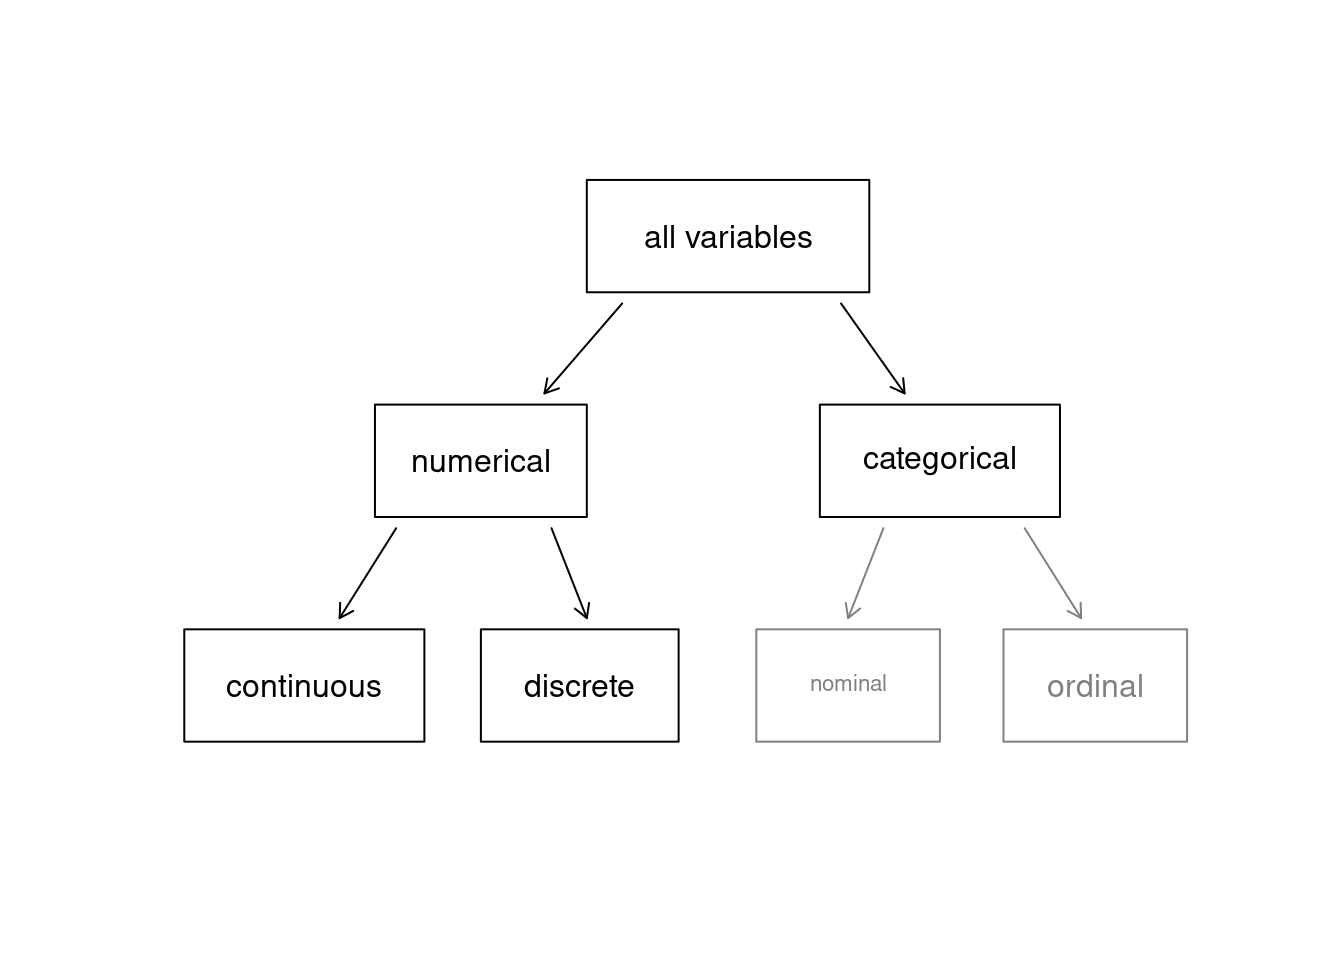
\includegraphics{02-Data-Basics_files/figure-latex/tax-fig-1.pdf}
\caption{\label{fig:tax-fig}Taxonomy of Variables.}
\end{figure}

Finally, consider a hypothetical variable on education, which describes the highest level of education completed and takes on one of the values \emph{noHS}, \emph{HS}, \emph{College} or \emph{Graduate\_school}. This variable seems to be a hybrid: it is a categorical variable but the levels have a natural ordering. A variable with these properties is called an \textbf{ordinal} variable. To simplify analyses, any ordinal variables in this course will be treated as categorical variables. In \texttt{R} categorical variables can be treated in different ways; one of the key differences is that we can leave them as character values or as factors. When \texttt{R} handles factors, it is only concerned about the \emph{levels} of values of the factors. We will learn more about this as the semester progresses.

Figure \ref{fig:tax-fig} captures this classification of variables.

\begin{quote}
\textbf{Exercise}:\\
Data were collected about students in a statistics course. Three variables were recorded for each student: number of siblings, student height, and whether the student had previously taken a statistics course. Classify each of the variables as continuous numerical, discrete numerical, or categorical.
\end{quote}

The number of siblings and student height represent numerical variables. Because the number of siblings is a count, it is discrete. Height varies continuously, so it is a continuous numerical variable. The last variable classifies students into two categories -- those who have and those who have not taken a statistics course -- which makes this variable categorical.

\begin{quote}
\textbf{Exercise}:\\
Consider the variables \texttt{group} and \texttt{outcome30} from the stent study in the case study lesson. Are these numerical or categorical variables? \footnote{There are only two possible values for each variable, and in both cases they describe categories. Thus, each is a categorical variable.}
\end{quote}

\hypertarget{relationships-between-variables}{%
\subsection{Relationships between variables}\label{relationships-between-variables}}

Many analyses are motivated by a researcher looking for a relationship between two or more variables, this is the heart of statistical modeling. A social scientist may like to answer some of the following questions:

\begin{enumerate}
\def\labelenumi{\arabic{enumi}.}
\tightlist
\item
  Is federal spending, on average, higher or lower in counties with high rates of poverty?\\
\item
  If homeownership is lower than the national average in one county, will the percent of multi-unit structures in that county likely be above or below the national average?
\end{enumerate}

To answer these questions, data must be collected, such as the \texttt{county\_complete} data set. Examining summary statistics could provide insights for each of the two questions about counties. Additionally, graphs can be used to visually summarize data and are useful for answering such questions as well.

Scatterplots are one type of graph used to study the relationship between two numerical variables. Figure \ref{fig:pov1-fig} compares the variables \texttt{fed\_spend} and \texttt{poverty}. Each point on the plot represents a single county. For instance, the highlighted dot corresponds to County 1088 in the \texttt{county\_M377} data set: Owsley County, Kentucky, which had a poverty rate of 41.5\% and federal spending of \$21.50 per capita. The dense cloud in the scatterplot suggests a relationship between the two variables: counties with a high poverty rate also tend to have slightly more federal spending. We might brainstorm as to why this relationship exists and investigate each idea to determine which is the most reasonable explanation.

\begin{figure}
\centering
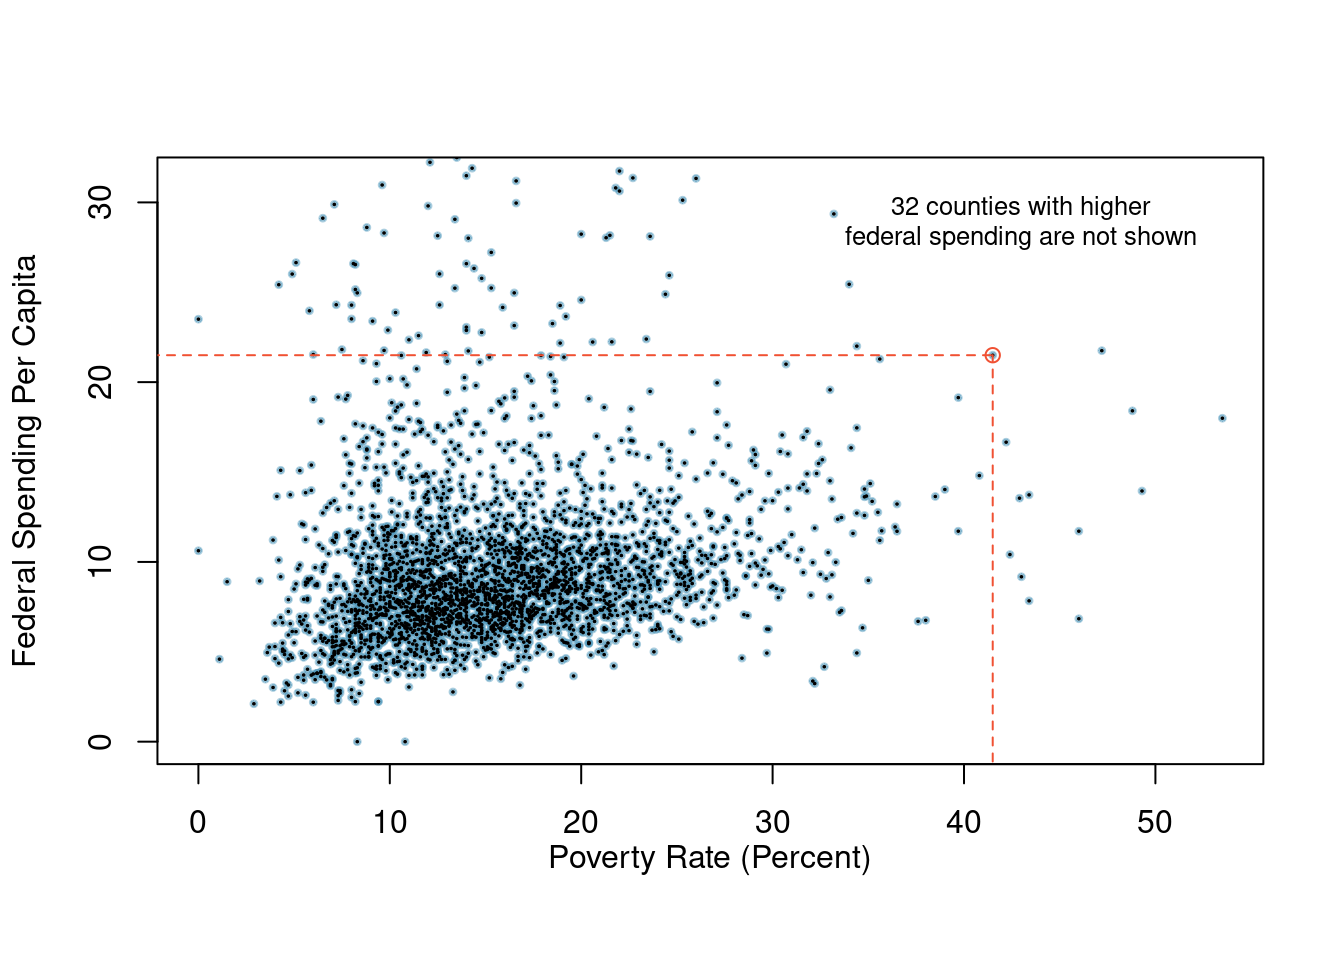
\includegraphics{02-Data-Basics_files/figure-latex/pov1-fig-1.pdf}
\caption{\label{fig:pov1-fig}A scatterplot showing fed\_spend against poverty. Owsley County of Kentucky, with a poverty rate of 41.5\% and federal spending of \$21.50 per capita, is highlighted.}
\end{figure}

\begin{quote}
\textbf{Exercise}:\\
Examine the variables in the \texttt{email50} data set. Create two questions about the relationships between these variables that are of interest to you.\footnote{Two sample questions: (1) Intuition suggests that if there are many line breaks in an email then there would also tend to be many characters: does this hold true? (2) Is there a connection between whether an email format is plain text (versus HTML) and whether it is a spam message?}
\end{quote}

The \texttt{fed\_spend} and \texttt{poverty} variables are said to be associated because the plot shows a discernible pattern. When two variables show some connection with one another, they are called \textbf{associated variables}. Associated variables can also be called \textbf{dependent} variables and vice-versa.

\begin{quote}
\emph{Example}:\\
The relationship between the homeownership rate and the percent of units in multi-unit structures (e.g.~apartments, condos) is visualized using a scatterplot in Figure \ref{fig:homeown-fig}. Are these variables associated?
\end{quote}

It appears that the larger the fraction of units in multi-unit structures, the lower the homeownership rate. Since there is some relationship between the variables, they are associated.

\begin{figure}
\centering
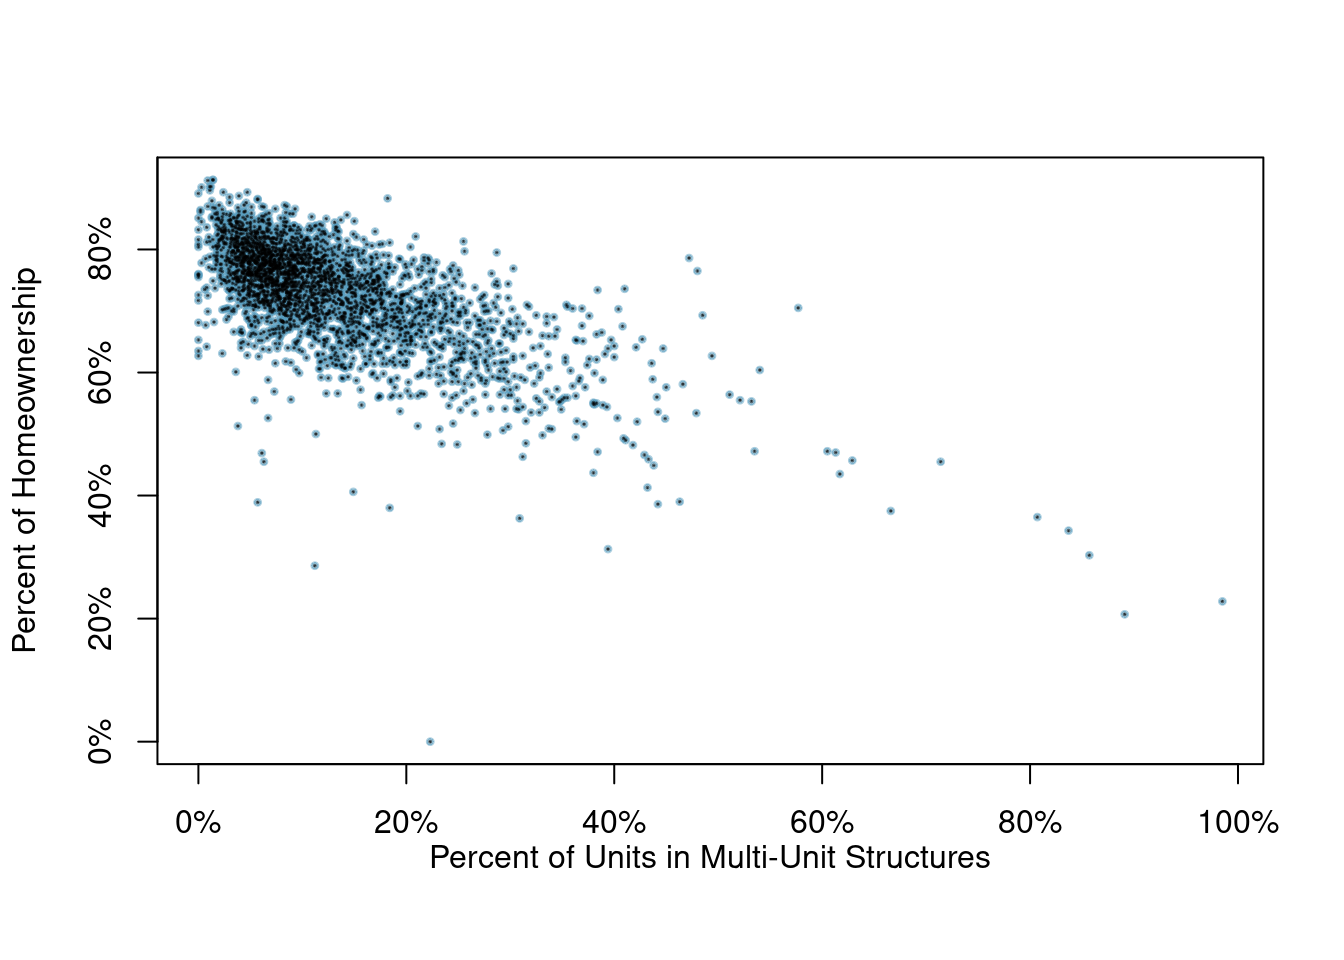
\includegraphics{02-Data-Basics_files/figure-latex/homeown-fig-1.pdf}
\caption{\label{fig:homeown-fig}A scatterplot of the homeownership rate versus the percent of units that are in multi-unit structures for all 3,143 counties.}
\end{figure}

Because there is a downward trend in Figure \ref{fig:homeown-fig} -- counties with more units in multi-unit structures are associated with lower homeownership -- these variables are said to be \textbf{negatively associated}. A \textbf{positive association} is shown in the relationship between the \texttt{poverty} and \texttt{fed\_spend} variables represented in Figure \ref{fig:pov1-fig}, where counties with higher poverty rates tend to receive more federal spending per capita.

If two variables are not associated, then they are said to be \textbf{independent}. That is, two variables are independent if there is no evident relationship between the two.

\begin{quote}
A pair of variables are either related in some way (associated) or not (independent). No pair of variables is both associated and independent.
\end{quote}

\hypertarget{creating-a-scatterplot}{%
\subsection{Creating a scatterplot}\label{creating-a-scatterplot}}

In this section we will create a simple scatterplot and then ask you to create one on your own. First we will recreate the scatterplot seen in Figure \ref{fig:pov1-fig}. This figure uses the \texttt{county\_M377} data set.

Here are two questions:

\emph{What do we want \texttt{R} to do?} and

\emph{What must we give \texttt{R} for it to do this?}

We want \texttt{R} to create a scatterplot and to do this it needs, at a minimum, the data object, what we want on the \(x\)-axis, and what we want on the \(y\)-axis. More information on \href{https://cran.r-project.org/web/packages/ggformula/vignettes/ggformula-blog.html}{\texttt{ggformula}} can be found by clicking on the link.\footnote{\url{https://cran.r-project.org/web/packages/ggformula/vignettes/ggformula-blog.html}}



\begin{Shaded}
\begin{Highlighting}[]
\NormalTok{county\_M377 }\SpecialCharTok{\%\textgreater{}\%}
  \FunctionTok{gf\_point}\NormalTok{(fed\_spend}\SpecialCharTok{\textasciitilde{}}\NormalTok{poverty)}
\end{Highlighting}
\end{Shaded}

\begin{figure}
\centering
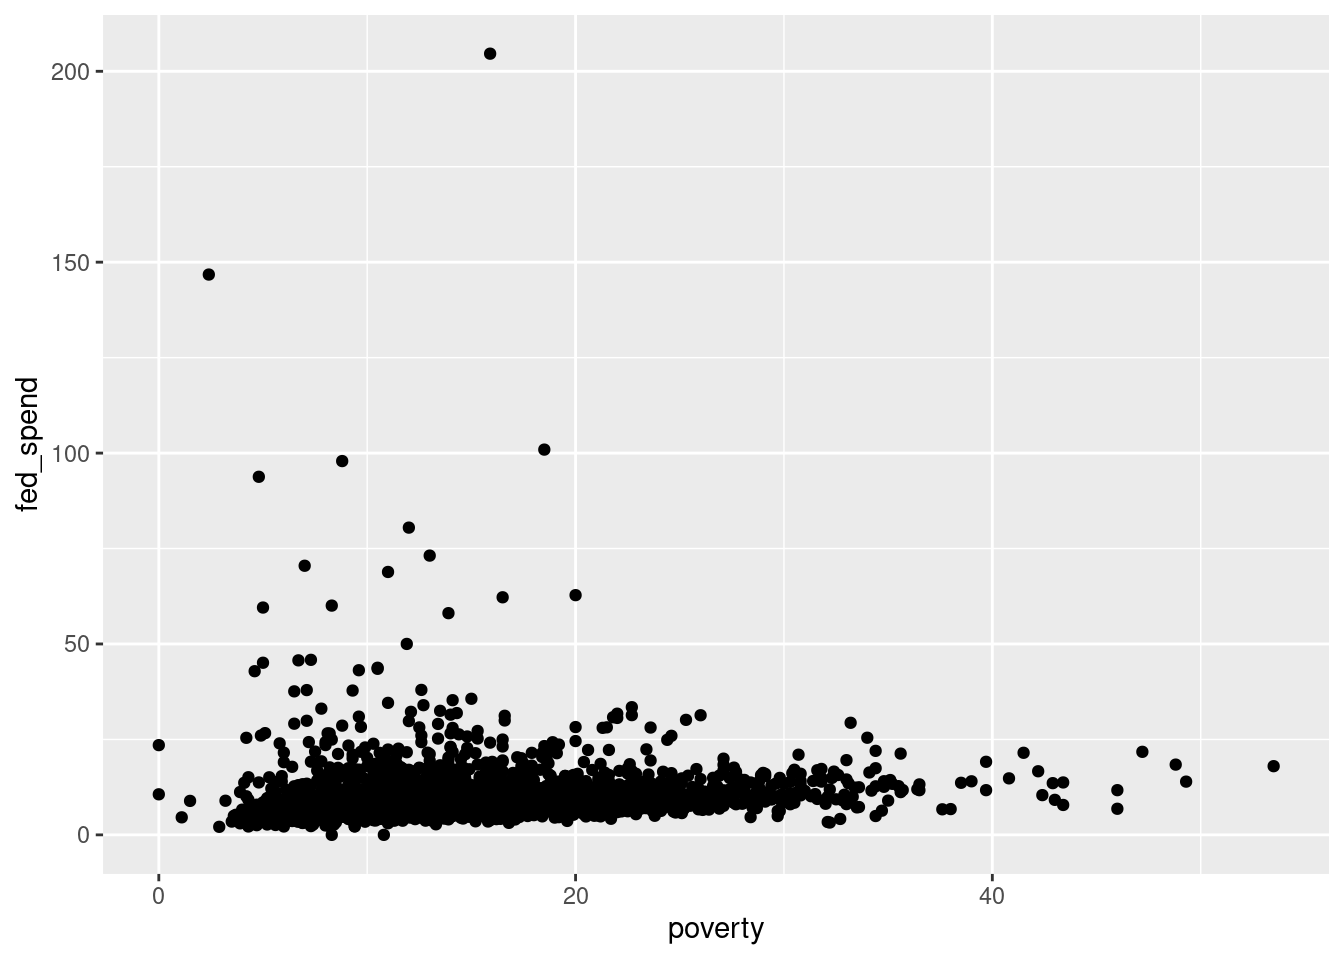
\includegraphics{02-Data-Basics_files/figure-latex/pov2-fig-1.pdf}
\caption{\label{fig:pov2-fig}Scatterplot with \textbf{ggformula}.}
\end{figure}

Figure \ref{fig:pov2-fig} is bad, there are poor axis labels, no title, dense clustering of points, the \(y\)-axis is being driven by a couple of extreme points. We will need to clear this up. Again, try to read the code and use \texttt{help()} or \texttt{?} to determine the purpose of each command in Figure \ref{fig:pov3-fig}.

\begin{Shaded}
\begin{Highlighting}[]
\NormalTok{county\_M377 }\SpecialCharTok{\%\textgreater{}\%}
  \FunctionTok{filter}\NormalTok{(fed\_spend}\SpecialCharTok{\textless{}}\DecValTok{32}\NormalTok{) }\SpecialCharTok{\%\textgreater{}\%}
  \FunctionTok{gf\_point}\NormalTok{(fed\_spend}\SpecialCharTok{\textasciitilde{}}\NormalTok{poverty,}
           \AttributeTok{xlab=}\StringTok{"Poverty Rate (Percent)"}\NormalTok{, }
           \AttributeTok{ylab=}\StringTok{"Federal Spending Per Capita"}\NormalTok{,}
           \AttributeTok{title=}\StringTok{"A scatterplot showing fed\_spend against poverty"}\NormalTok{, }
           \AttributeTok{subtitle =}  \StringTok{"Owsley County of Kentucky"}\NormalTok{,}
           \AttributeTok{cex=}\DecValTok{1}\NormalTok{,}\AttributeTok{alpha=}\FloatTok{0.2}\NormalTok{) }\SpecialCharTok{\%\textgreater{}\%}
  \FunctionTok{gf\_theme}\NormalTok{(}\FunctionTok{theme\_classic}\NormalTok{())}
\end{Highlighting}
\end{Shaded}

\begin{figure}
\centering
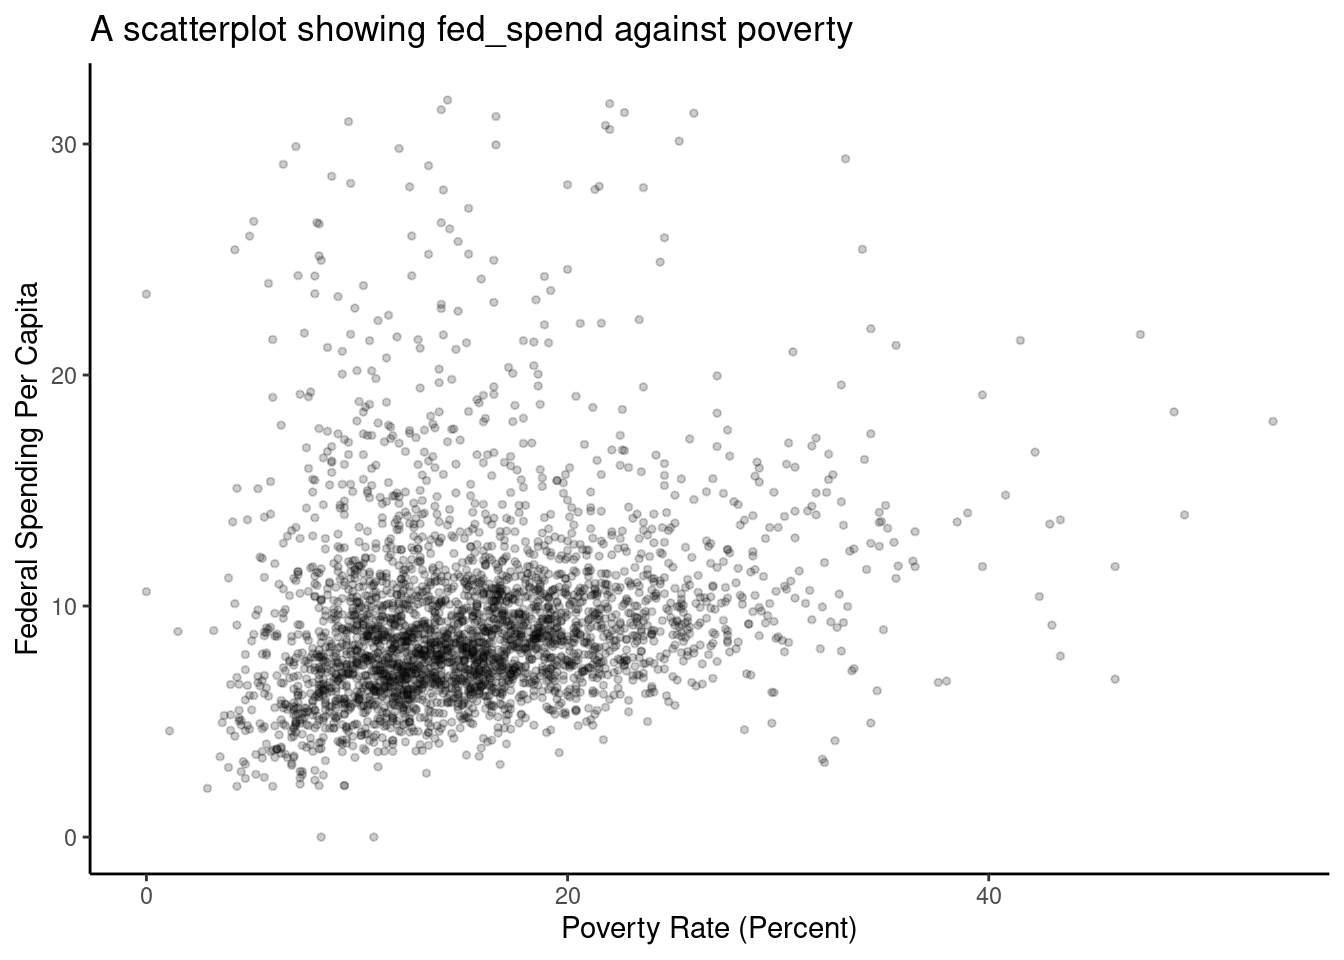
\includegraphics{02-Data-Basics_files/figure-latex/pov3-fig-1.pdf}
\caption{\label{fig:pov3-fig}Better example of a scatterplot.}
\end{figure}

\begin{quote}
\textbf{Exercise}:\\
Create the scatterplot in Figure \ref{fig:homeown-fig}.
\end{quote}

\hypertarget{homework-problems-1}{%
\section{Homework Problems}\label{homework-problems-1}}

\textbf{Identify study components}

Identify (i) the cases, (ii) the variables and their types, and (iii) the main research question in the studies described below.

\begin{enumerate}
\def\labelenumi{\arabic{enumi}.}
\item
  Researchers collected data to examine the relationship between pollutants and preterm births in Southern California. During the study air pollution levels were measured by air quality monitoring stations. Specifically, levels of carbon monoxide were recorded in parts per million, nitrogen dioxide and ozone in parts per hundred million, and coarse particulate matter (PM\(_{10}\)) in \(\mu g/m^3\). Length of gestation data were collected on 143,196 births between the years 1989 and 1993, and air pollution exposure during gestation was calculated for each birth. The analysis suggested that increased ambient PM\(_{10}\) and, to a lesser degree, CO concentrations may be associated with the occurrence of preterm births.\footnote{B. Ritz et al.~\href{http://journals.lww.com/epidem/Abstract/2000/09000/Effect_of_Air_Pollution_on_Preterm_Birth_Among.4.aspx}{``Effect of air pollution on preterm birth among children born in Southern California
    between 1989 and 1993''}. In: Epidemiology 11.5 (2000), pp.~502--511.}
\item
  The Buteyko method is a shallow breathing technique developed by Konstantin Buteyko, a Russian doctor, in 1952. Anecdotal evidence suggests that the Buteyko method can reduce asthma symptoms and improve quality of life. In a scientific study to determine the effectiveness of this method, researchers recruited 600 asthma patients aged 18-69 who relied on medication for asthma treatment. These patients were split into two research groups: one practiced the Buteyko method and the other did not. Patients were scored on quality of life, activity, asthma symptoms, and medication reduction on a scale from 0 to 10. On average, the participants in the Buteyko group experienced a significant reduction in asthma symptoms and an improvement in quality of life.\footnote{J. McGowan. ``Health Education: Does the Buteyko Institute Method make a difference?'' In: Thorax 58 (2003).}
\end{enumerate}

\hypertarget{ODCP}{%
\chapter{Overview of Data Collection Principles}\label{ODCP}}

\hypertarget{objectives-2}{%
\section{Objectives}\label{objectives-2}}

\begin{enumerate}
\def\labelenumi{\arabic{enumi})}
\tightlist
\item
  Define and use properly in context all new terminology.\\
\item
  From a description of a research project, at a minimum be able to describe the population of interest, the generalizability of the study, the response and predictor variables, differentiate whether it is observational or experimental, and determine the type of sample.
\end{enumerate}

\hypertarget{overview-of-data-collection-principles}{%
\section{Overview of data collection principles}\label{overview-of-data-collection-principles}}

The first step in conducting research is to identify topics or questions that are to be investigated. A clearly laid out research question is helpful in identifying what subjects or cases should be studied and what variables are important. It is also important to consider \emph{how} data are collected so that they are reliable and help achieve the research goals.

\hypertarget{populations-and-samples}{%
\subsection{Populations and samples}\label{populations-and-samples}}

Consider the following three research questions:

\begin{enumerate}
\def\labelenumi{\arabic{enumi}.}
\tightlist
\item
  What is the average mercury content in swordfish in the Atlantic Ocean?\\
\item
  Over the last 5 years, what is the average time to complete a degree for Duke undergraduate students?\\
\item
  Does a new drug reduce the number of deaths in patients with severe heart disease?
\end{enumerate}

Each research question refers to a target \textbf{population}. In the first question, the target population is all swordfish in the Atlantic Ocean, and each fish represents a case. It is usually too expensive to collect data for every case in a population. Instead, a sample is taken. A \textbf{sample} represents a subset of the cases and is often a small fraction of the population. For instance, 60 swordfish (or some other number) in the population might be selected, and this sample data may be used to provide an estimate of the population average and answer the research question.

\begin{quote}
\textbf{Exercise}:\\
For the second and third questions above, identify the target population and what represents an individual case.\footnote{ 2) Notice that the first question is only relevant to students who complete their degree; the average cannot be computed using a student who never finished her degree. Thus, only Duke undergraduate students who have graduated in the last five years represent cases in the population under consideration. Each such student would represent an individual case. 3) A person with severe heart disease represents a case. The population includes all people with severe heart disease.}
\end{quote}

\hypertarget{anecdotal-evidence}{%
\subsection{Anecdotal evidence}\label{anecdotal-evidence}}

Consider the following possible responses to the three research questions:

\begin{enumerate}
\def\labelenumi{\arabic{enumi}.}
\tightlist
\item
  A man on the news got mercury poisoning from eating swordfish, so the average mercury concentration in swordfish must be dangerously high.
\item
  I met two students who took more than 7 years to graduate from Duke, so it must take longer to graduate at Duke than at many other colleges.
\item
  My friend's dad had a heart attack and died after they gave him a new heart disease drug, so the drug must not work.
\end{enumerate}

Each conclusion is based on data. However, there are two problems. First, the data only represent one or two cases. Second, and more importantly, it is unclear whether these cases are actually representative of the population. Data collected in this haphazard fashion are called \textbf{anecdotal evidence}.



\begin{figure}

{\centering 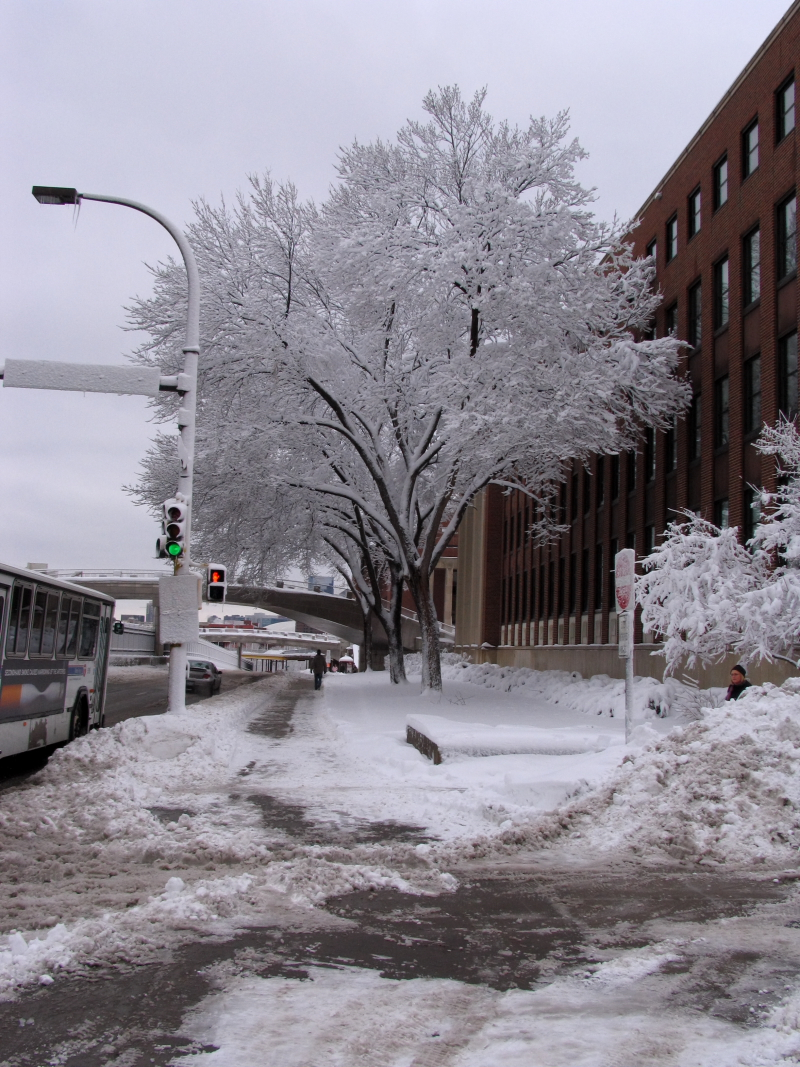
\includegraphics[width=11.11in]{./figures/mnWinter} 

}

\caption{In February 2010, some media pundits cited one large snow storm as evidence against global warming. As comedian Jon Stewart pointed out, \emph{`It's one storm, in one region, of one country.'}}\label{fig:unnamed-chunk-1}
\end{figure}

\begin{quote}
\textbf{Anecdotal evidence}:
Be careful of data collected haphazardly. Such evidence may be true and verifiable, but it may only represent extraordinary cases.
\end{quote}

Anecdotal evidence typically is composed of unusual cases that we recall based on their striking characteristics. For instance, we are more likely to remember the two people we met who took 7 years to graduate than the six others who graduated in four years. Instead of looking at the most unusual cases, we should examine a sample of many cases that represent the population.

\hypertarget{sampling-from-a-population}{%
\subsection{Sampling from a population}\label{sampling-from-a-population}}

We might try to estimate the time to graduation for Duke undergraduates in the last 5 years by collecting a sample of students. All graduates in the last 5 years represent the \emph{population}, and graduates who are selected for review are collectively called the \emph{sample}. In general, we always seek to \emph{randomly} select a sample from a population. The most basic type of random selection is equivalent to how raffles are conducted. For example, in selecting graduates, we could write each graduate's name on a raffle ticket and draw 100 tickets. The selected names would represent a random sample of 100 graduates. This is illustrated in Figure \ref{fig:randsamp-fig}.

\begin{figure}
\centering
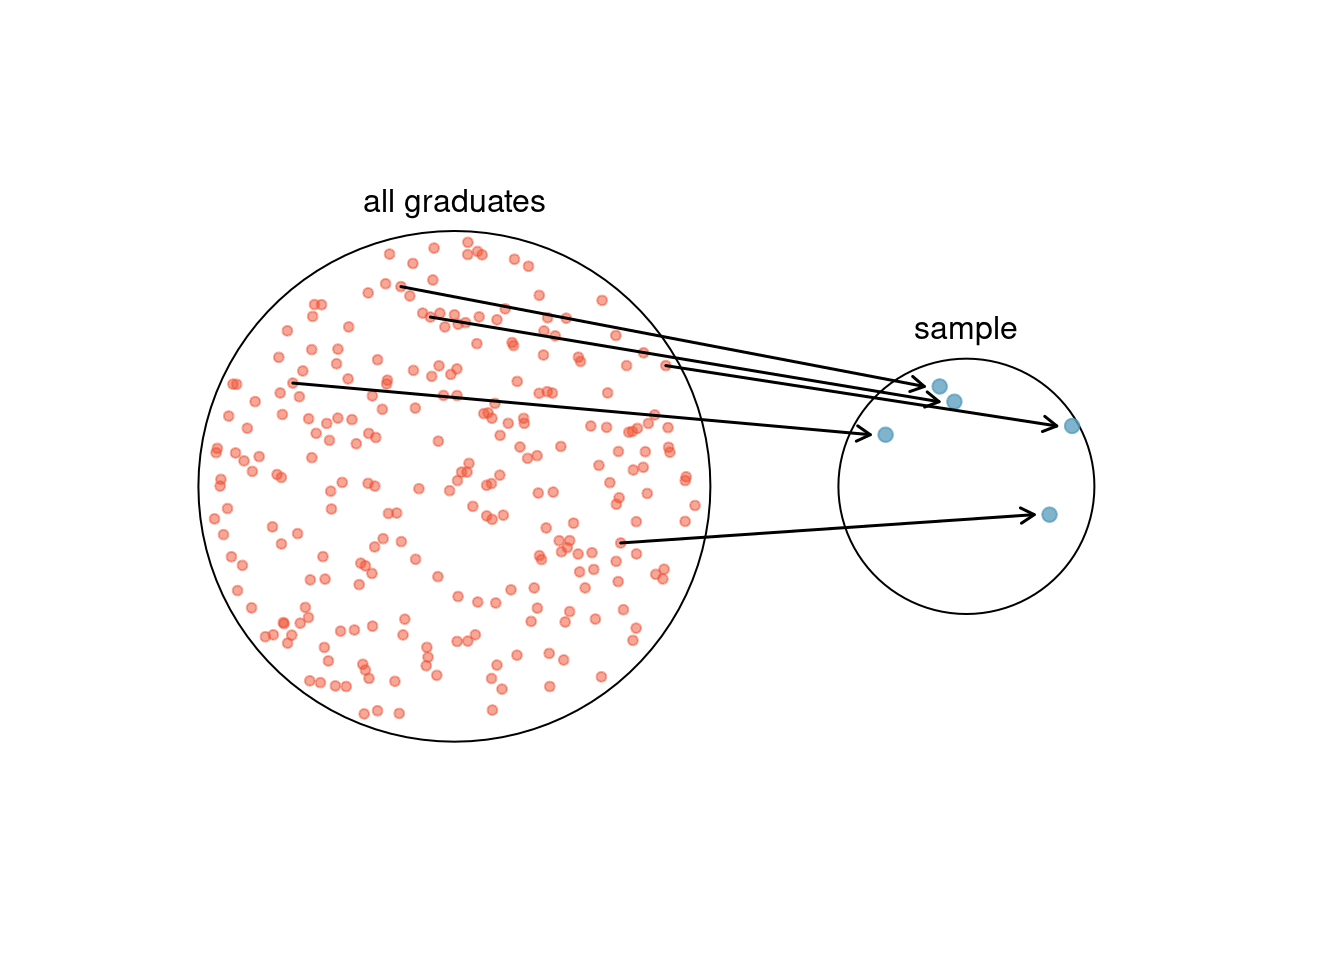
\includegraphics{03-Overview-of-Data-Collection-Principles_files/figure-latex/randsamp-fig-1.pdf}
\caption{\label{fig:randsamp-fig}In this graphic, five graduates are randomly selected from the population to be included in the sample.}
\end{figure}

Why pick a sample randomly? Why not just pick a sample by hand? Consider the following scenario.

\begin{quote}
\textbf{Example}:\\
Suppose we ask a student who happens to be majoring in nutrition to select several graduates for the study. What kind of students do you think she might collect? Do you think her sample would be representative of all graduates?
\footnote{Perhaps she would pick a disproportionate number of graduates from health-related fields. Or perhaps her selection would be well-representative of the population. When selecting samples by hand, we run the risk of picking a \emph{biased} sample, even if that bias is unintentional or difficult to discern.}
\end{quote}

\begin{figure}
\centering
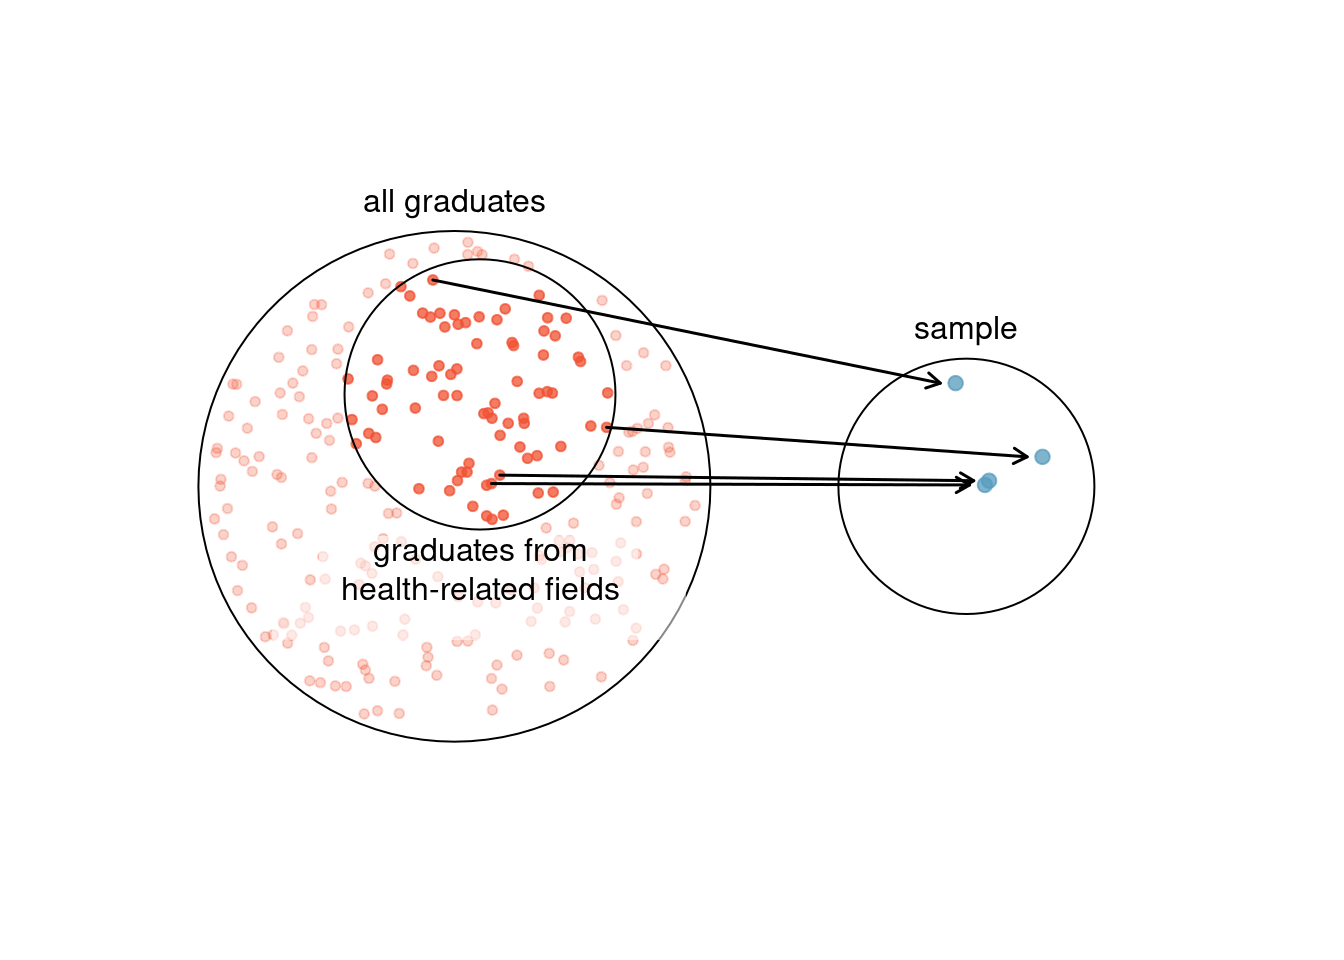
\includegraphics{03-Overview-of-Data-Collection-Principles_files/figure-latex/biased-fig-1.pdf}
\caption{\label{fig:biased-fig}Instead of sampling from all graduates equally, a nutrition major might inadvertently pick graduates with health-related majors disproportionately often.}
\end{figure}

If someone was permitted to pick and choose exactly which graduates were included in the sample, it is entirely possible that the sample could be skewed to that person's interests, which may be entirely unintentional. This introduces \textbf{bias} into a sample, see Figure \ref{fig:biased-fig}. Sampling randomly helps resolve this problem. The most basic random sample is called a \textbf{simple random sample}, which is equivalent to using a raffle to select cases. This means that each case in the population has an equal chance of being included and there is no implied connection between the cases in the sample.

Sometimes a simple random sample is difficult to implement and an alternative method is helpful. One such substitute is a \textbf{systematic sample}, where one case is sampled after letting a fixed number of others, say 10 other cases, pass by. Since this approach uses a mechanism that is not easily subject to personal biases, it often yields a reasonably representative sample. This course will focus on simple random samples since the use of systematic samples is uncommon and requires additional considerations of the context.

The act of taking a simple random sample helps minimize bias. However, bias can crop up in other ways. Even when people are picked at random, e.g.~for surveys, caution must be exercised if the \textbf{non-response} is high. For instance, if only 30\% of the people randomly sampled for a survey actually respond, and it is unclear whether the respondents are \textbf{representative} of the entire population, the survey might suffer from \textbf{non-response bias}.

\begin{figure}
\centering
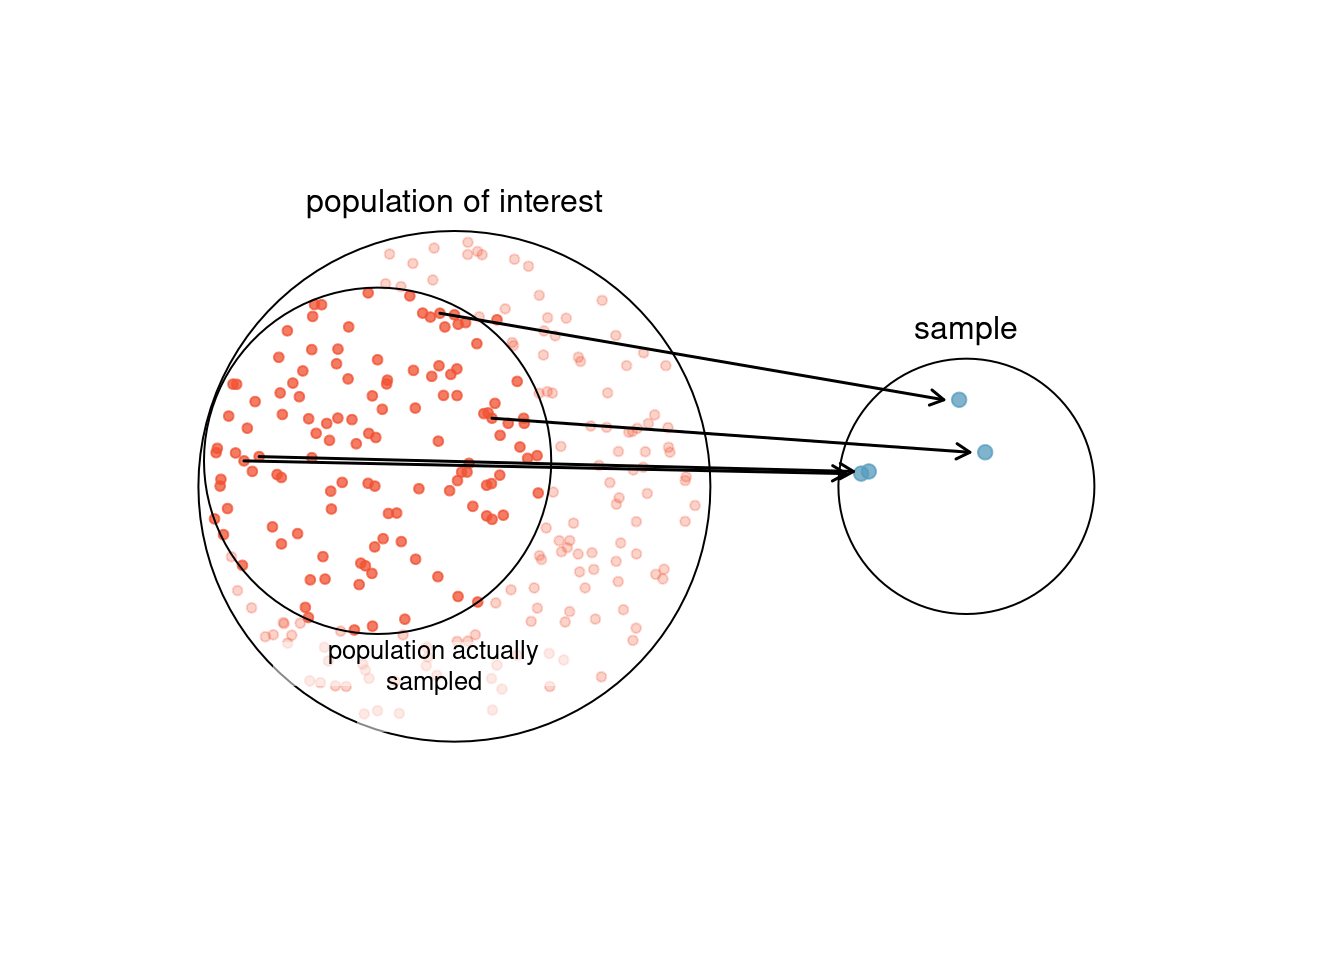
\includegraphics{03-Overview-of-Data-Collection-Principles_files/figure-latex/convsamp-fig-1.pdf}
\caption{\label{fig:convsamp-fig}Due to the possibility of non-response, surveys studies may only reach a certain group within the population. It is difficult, and often impossible, to completely fix this problem}
\end{figure}

Another common pitfall is a \textbf{convenience sample}, where individuals who are easily accessible are more likely to be included in the sample, see Figure \ref{fig:convsamp-fig} . For instance, if a political survey is done by stopping people walking in the Bronx, it will not represent all of New York City. It is often difficult to discern what sub-population a convenience sample represents.

\begin{quote}
\textbf{Exercise}:\\
We can easily access ratings for products, sellers, and companies through websites. These ratings are based only on those people who go out of their way to provide a rating. If 50\% of online reviews for a product are negative, do you think this means that 50\% of buyers are dissatisfied with the product?\footnote{Answers will vary. From our own anecdotal experiences, we believe people tend to rant more about products that fell below expectations than rave about those that perform as expected. For this reason, we suspect there is a negative bias in product ratings on sites like Amazon. However, since our experiences may not be representative, we also keep an open mind.}
\end{quote}

\hypertarget{explanatory-and-response-variables}{%
\subsection{Explanatory and response variables}\label{explanatory-and-response-variables}}

Consider the following question for the \texttt{county} data set:

Is federal spending, on average, higher or lower in counties with high rates of poverty?

If we suspect poverty might affect spending in a county, then poverty is the \textbf{explanatory} variable and federal spending is the \textbf{response} variable in the relationship.\footnote{Sometimes the explanatory variable is called the \textbf{independent} variable and the response variable is called the \textbf{dependent} variable. However, this becomes confusing since a \emph{pair} of variables might be independent or dependent, so be careful and consider the context when using or reading these words.} If there are many variables, it may be possible to consider a number of them as explanatory variables.

\begin{quote}
\textbf{Explanatory} and \textbf{response} variables\\
To identify the explanatory variable in a pair of variables, identify which of the two is suspected of affecting the other.
\end{quote}

\begin{quote}
\textbf{Caution}:
Association does not imply causation. Labeling variables as \emph{explanatory} and \emph{response} does not guarantee the relationship between the two is actually causal, even if there is an association identified between the two variables. We use these labels only to keep track of which variable we suspect affects the other. We also use this language to help in our use of \texttt{R} and the formula notation.
\end{quote}

In some cases, there is no explanatory or response variable. Consider the following question:

If homeownership in a particular county is lower than the national average, will the percent of multi-unit structures in that county likely be above or below the national average?

It is difficult to decide which of these variables should be considered the explanatory and response variable; i.e.~the direction is ambiguous, so no explanatory or response labels are suggested here.

\hypertarget{introducing-observational-studies-and-experiments}{%
\subsection{Introducing observational studies and experiments}\label{introducing-observational-studies-and-experiments}}

There are two primary types of data collection: observational studies and experiments.

Researchers perform an \textbf{observational study} when they collect data in a way that does not directly interfere with how the data arise. For instance, researchers may collect information via surveys, review medical or company records, or follow a \textbf{cohort} of many similar individuals to study why certain diseases might develop. In each of these situations, researchers merely observe what happens. In general, observational studies can provide evidence of a naturally occurring association between variables, but by themselves, they cannot show a causal connection.

When researchers want to investigate the possibility of a causal connection, they conduct an \textbf{experiment}. Usually there will be both an explanatory and a response variable. For instance, we may suspect administering a drug will reduce mortality in heart attack patients over the following year. To check if there really is a causal connection between the explanatory variable and the response, researchers will collect a sample of individuals and split them into groups. The individuals in each group are \emph{assigned} a treatment. When individuals are randomly assigned to a treatment group, the experiment is called a \textbf{randomized experiment}. For example, each heart attack patient in the drug trial could be randomly assigned, perhaps by flipping a coin, into one of two groups: the first group receives a \textbf{placebo} (fake treatment) and the second group receives the drug. The case study at the beginning of the semester is another example of an experiment, though that study did not employ a placebo. Math 359 is a course on the design and analysis of experimental data, DOE. In the Air Force these types of experiments are an important part of test and evaluation. Many Air Force analysts are expert practitioners of DOE. In this course we will minimize our discussion of DOE.

\begin{quote}
Association \(\neq\) Causation\\
Again, association does not imply causation. In a data analysis, association does not imply causation, and causation can only be inferred from a randomized experiment. Although, a hot field is the analysis of causal relationships in observational data. This is important because consider cigarette smoking, how do we know it causes lung cancer? We only have observational data and clearly cannot do an experiment. We think analysts will be charged in the near future with using causal reasoning on observational data.
\end{quote}

\hypertarget{homework-problems-2}{%
\section{Homework Problems}\label{homework-problems-2}}

\begin{enumerate}
\def\labelenumi{\arabic{enumi}.}
\tightlist
\item
  \textbf{Generalizability and causality}. Identify the population of interest and the sample in the studies described below. These are the same studies from the previous lesson. Also comment on whether or not the results of the study can be generalized to the population and if the findings of the study can be used to establish causal relationships.
\end{enumerate}

\begin{enumerate}
\def\labelenumi{\alph{enumi}.}
\tightlist
\item
  Researchers collected data to examine the relationship between pollutants and preterm births in Southern California. During the study air pollution levels were measured by air quality monitoring stations. Specifically, levels of carbon monoxide were recorded in parts per million, nitrogen dioxide and ozone in parts per hundred million, and coarse particulate matter (PM\(_{10}\)) in \(\mu g/m^3\). Length of gestation data were collected on 143,196 births between the years 1989 and 1993, and air pollution exposure during gestation was calculated for each birth. The analysis suggested that increased ambient PM\(_{10}\) and, to a lesser degree, CO concentrations may be associated with the occurrence of preterm births.\footnote{B. Ritz et al.~\href{http://journals.lww.com/epidem/Abstract/2000/09000/Effect_of_Air_Pollution_on_Preterm_Birth_Among.4.aspx}{``Effect of air pollution on preterm birth among children born in Southern California
    between 1989 and 1993''}. In: Epidemiology 11.5 (2000), pp.~502--511.}\\
\item
  The Buteyko method is a shallow breathing technique developed by Konstantin Buteyko, a Russian doctor, in 1952. Anecdotal evidence suggests that the Buteyko method can reduce asthma symptoms and improve quality of life. In a scientific study to determine the effectiveness of this method, researchers recruited 600 asthma patients aged 18-69 who relied on medication for asthma treatment. These patients were split into two research groups: one practiced the Buteyko method and the other did not. Patients were scored on quality of life, activity, asthma symptoms, and medication reduction on a scale from 0 to 10. On average, the participants in the Buteyko group experienced a significant reduction in asthma symptoms and an improvement in quality of life.\footnote{J. McGowan. ``Health Education: Does the Buteyko Institute Method make a difference?'' In: Thorax 58 (2003).}
\end{enumerate}

\pagebreak

\begin{enumerate}
\def\labelenumi{\arabic{enumi}.}
\setcounter{enumi}{1}
\tightlist
\item
  \textbf{GPA and study time}. A survey was conducted on 55 undergraduates from Duke University who took an introductory statistics course in Spring 2012. Among many other questions, this survey asked them about their GPA and the number of hours they spent studying per week. The scatterplot below displays the relationship between these two variables.
\end{enumerate}

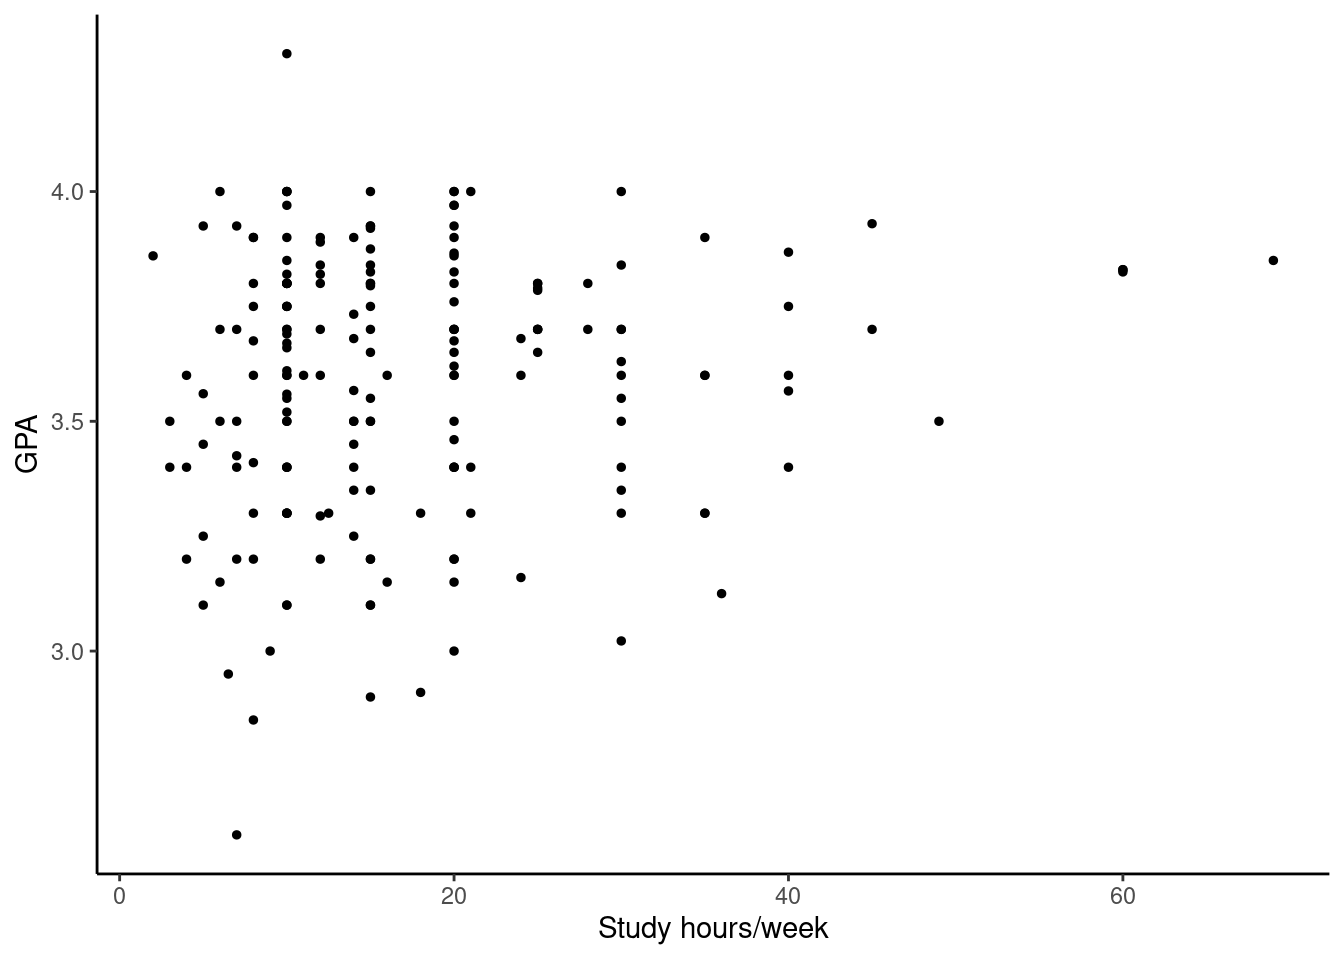
\includegraphics{03-Overview-of-Data-Collection-Principles_files/figure-latex/unnamed-chunk-2-1.pdf}

\begin{enumerate}
\def\labelenumi{\alph{enumi}.}
\tightlist
\item
  What is the explanatory variable and what is the response variable?
\item
  Describe the relationship between the two variables. Make sure to discuss unusual observations, if any.
\item
  Is this an experiment or an observational study?
\item
  Can we conclude that studying longer hours leads to higher GPAs?
\end{enumerate}

\pagebreak

\begin{enumerate}
\def\labelenumi{\arabic{enumi}.}
\setcounter{enumi}{2}
\tightlist
\item
  \textbf{Income and education} The scatterplot below shows the relationship between per capita income (in thousands of dollars) and percent of population with a bachelor's degree in 3,143 counties in the US in 2010.
\end{enumerate}

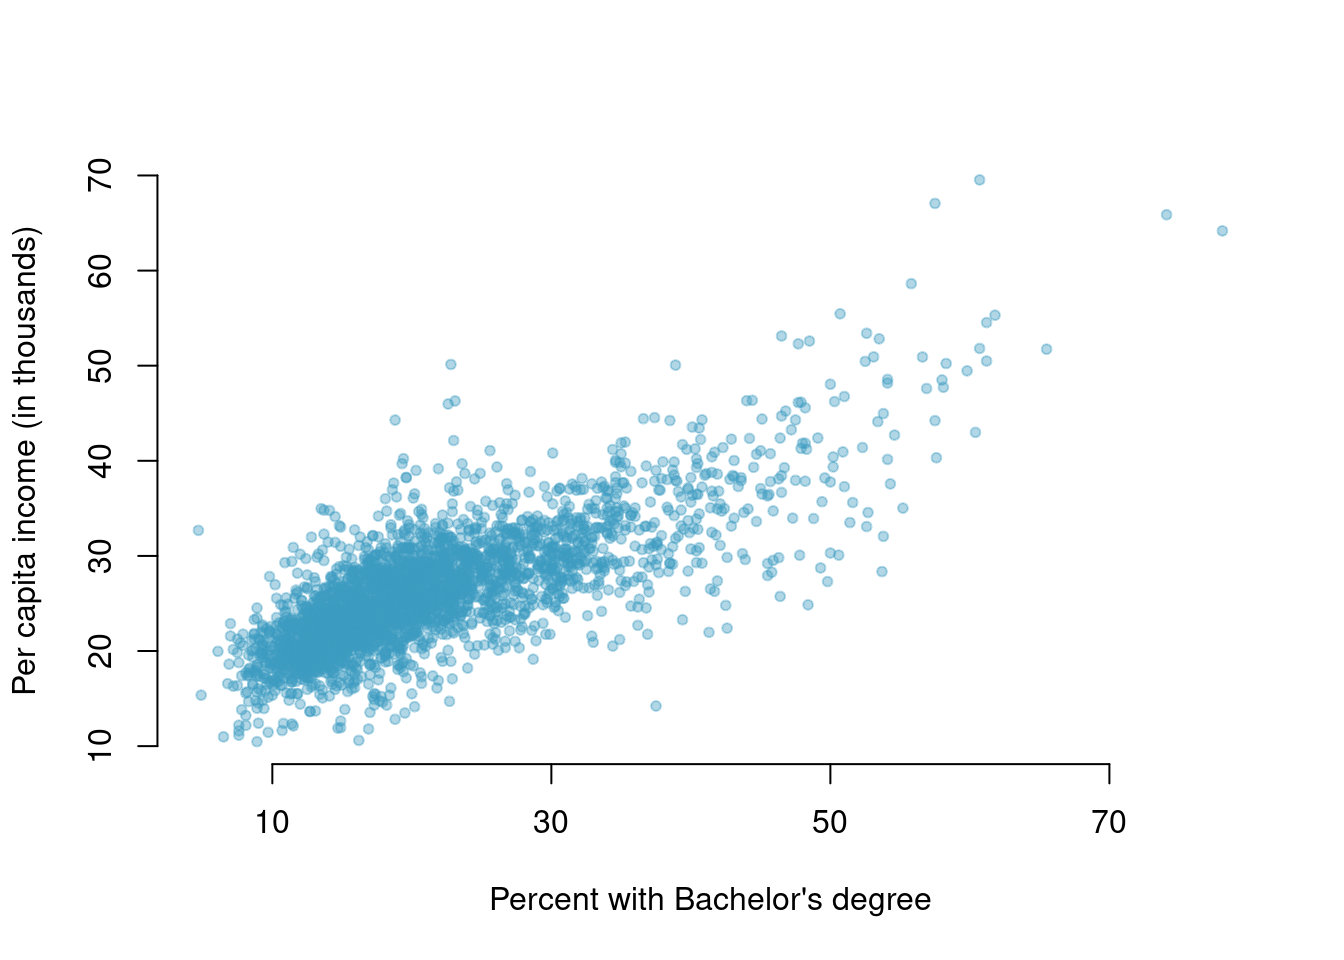
\includegraphics{03-Overview-of-Data-Collection-Principles_files/figure-latex/unnamed-chunk-3-1.pdf}

\begin{enumerate}
\def\labelenumi{\alph{enumi}.}
\tightlist
\item
  What are the explanatory and response variables?\\
\item
  Describe the relationship between the two variables. Make sure to discuss unusual observations, if any.\\
\item
  Can we conclude that having a bachelor's degree increases one's income?
\end{enumerate}

\hypertarget{STUDY}{%
\chapter{Studies}\label{STUDY}}

\hypertarget{objectives-3}{%
\section{Objectives}\label{objectives-3}}

\begin{enumerate}
\def\labelenumi{\arabic{enumi})}
\tightlist
\item
  Define and use properly in context all new terminology.\\
\item
  Given a study description, be able to identify and explain the study using correct terms.\\
\item
  Given a scenario, describe flaws in reasoning and propose study and sampling designs.
\end{enumerate}

\hypertarget{observation-studies-sampling-strategies-and-experiments}{%
\section{Observation studies, sampling strategies, and experiments}\label{observation-studies-sampling-strategies-and-experiments}}

\hypertarget{observational-studies}{%
\subsection{Observational studies}\label{observational-studies}}

Generally, data in observational studies are collected only by monitoring what occurs, while experiments require the primary explanatory variable in a study be assigned for each subject by the researchers.

Making causal conclusions based on experiments is often reasonable. However, making the same causal conclusions based on observational data can be treacherous and is not recommended. Thus, observational studies are generally only sufficient to show associations.

\begin{quote}
\textbf{Exercise}:\\
Suppose an observational study tracked sunscreen use and skin cancer, and it was found that the more sunscreen someone used, the more likely the person was to have skin cancer. Does this mean sunscreen \emph{causes} skin cancer?\footnote{No.~See the paragraph following the exercise for an explanation.}
\end{quote}

Some previous research\footnote{\url{http://www.sciencedirect.com/science/article/pii/S0140673698121682}~\\
  \url{http://archderm.ama-assn.org/cgi/content/abstract/122/5/537}~\\
  Study with a similar scenario to that described here:\\
  \url{http://onlinelibrary.wiley.com/doi/10.1002/ijc.22745/full}} tells us that using sunscreen actually reduces skin cancer risk, so maybe there is another variable that can explain this hypothetical association between sunscreen usage and skin cancer. One important piece of information that is absent is sun exposure. If someone is out in the sun all day, she is more likely to use sunscreen \emph{and} more likely to get skin cancer. Exposure to the sun is unaccounted for in the simple investigation.

\begin{figure}
\centering
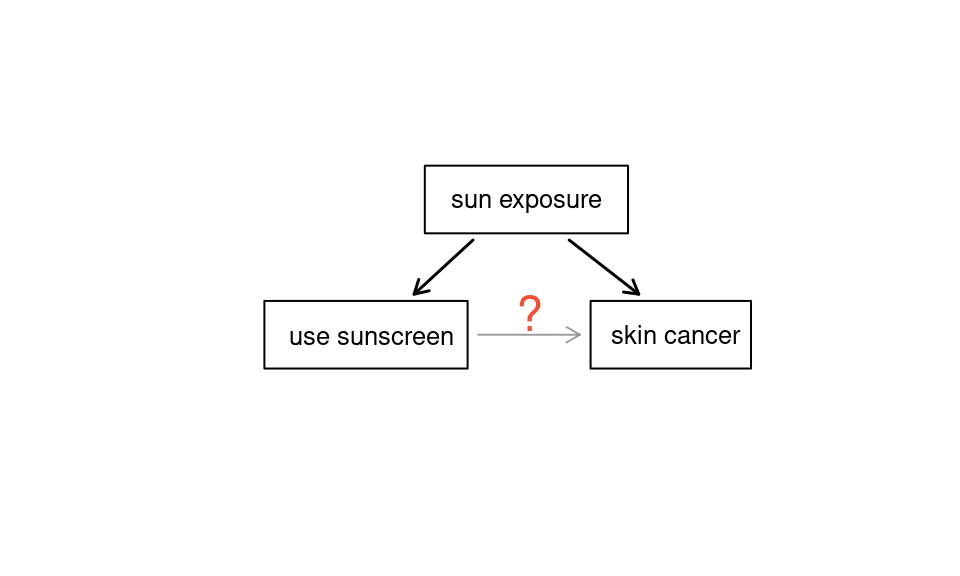
\includegraphics{04-Studies_files/figure-latex/confound-fig-1.pdf}
\caption{\label{fig:confound-fig}Sun exposure is a confounding variable because it is related to both response and explanatory variables.}
\end{figure}

Sun exposure is what is called a \textbf{confounding variable},\footnote{Also called a \textbf{lurking variable}, \textbf{confounding factor}, or a \textbf{confounder}.} which is a variable that is correlated with both the explanatory and response variables, see Figure \ref{fig:confound-fig} . While one method to justify making causal conclusions from observational studies is to exhaust the search for confounding variables, there is no guarantee that all confounding variables can be examined or measured.

Let's look at an example of confounding visually. Using the \texttt{SAT} data from the \textbf{mosaic} package let's look at expenditure per pupil versus SAT scores. Figure \ref{fig:confound2-fig} is a plot of the data.

\begin{quote}
\textbf{Exercise}:\\
What conclusion to you reach from the plot in Figure \ref{fig:confound2-fig}?\footnote{It appears that average SAT score declines as expenditures per student increases.}
\end{quote}

\begin{figure}
\centering
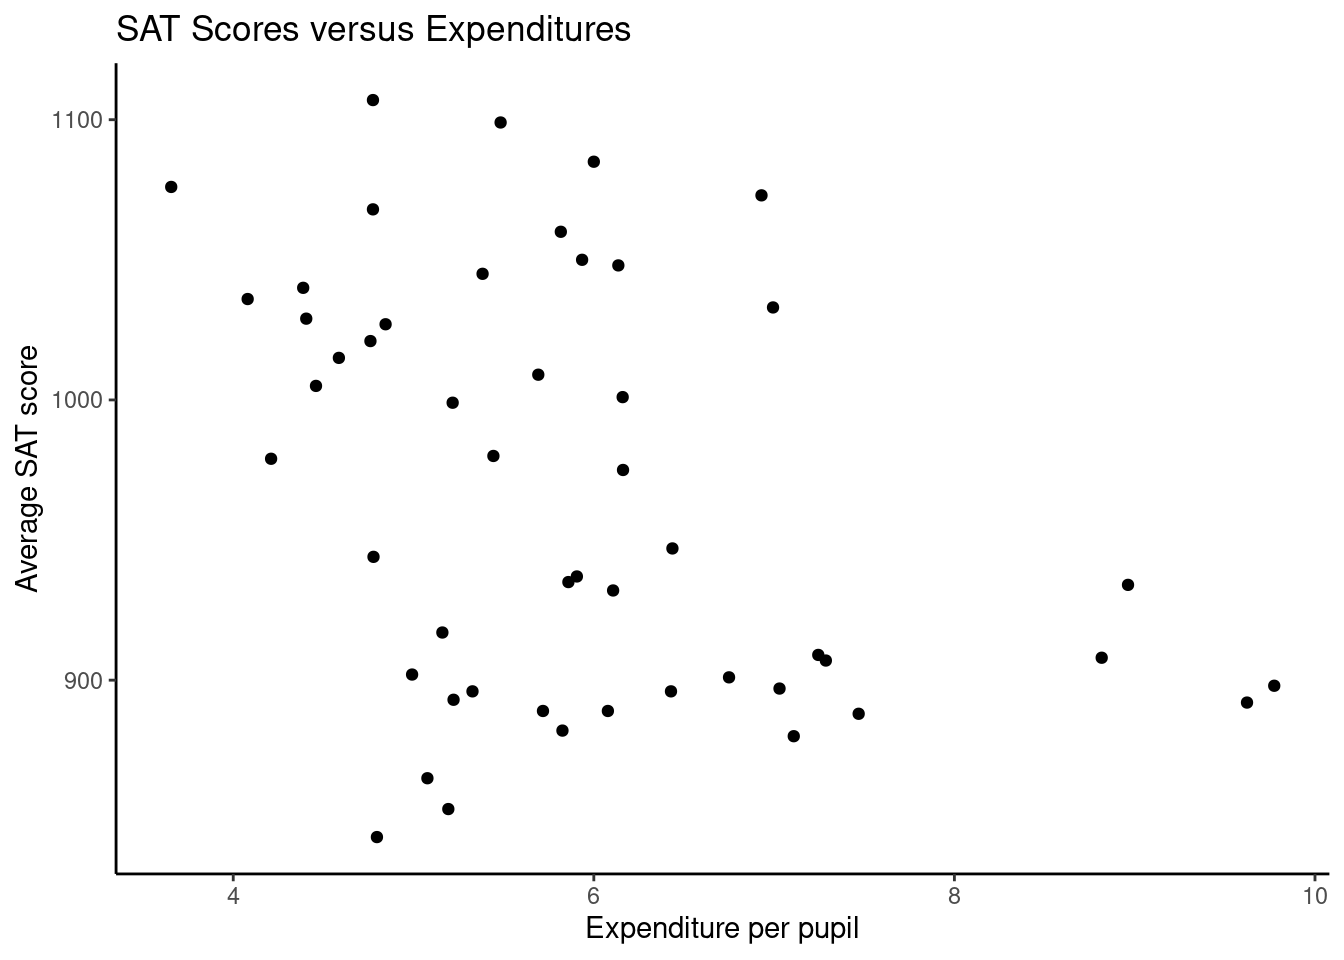
\includegraphics{04-Studies_files/figure-latex/confound2-fig-1.pdf}
\caption{\label{fig:confound2-fig}Average SAT score versus expenditure per pupil; reminder: each observation represents an individual state.}
\end{figure}

The implication that spending less might give better results is not justified. Expenditures are confounded with the proportion of students who take the exam, and scores are higher in states where fewer students take the exam.

It is interesting to look at the original plot if we place the states into two groups depending on whether more or
fewer than 40\% of students take the SAT. Figure \ref{fig:conditional-fig} is a plot of the data broken down into the 2 groups.

\begin{figure}
\centering
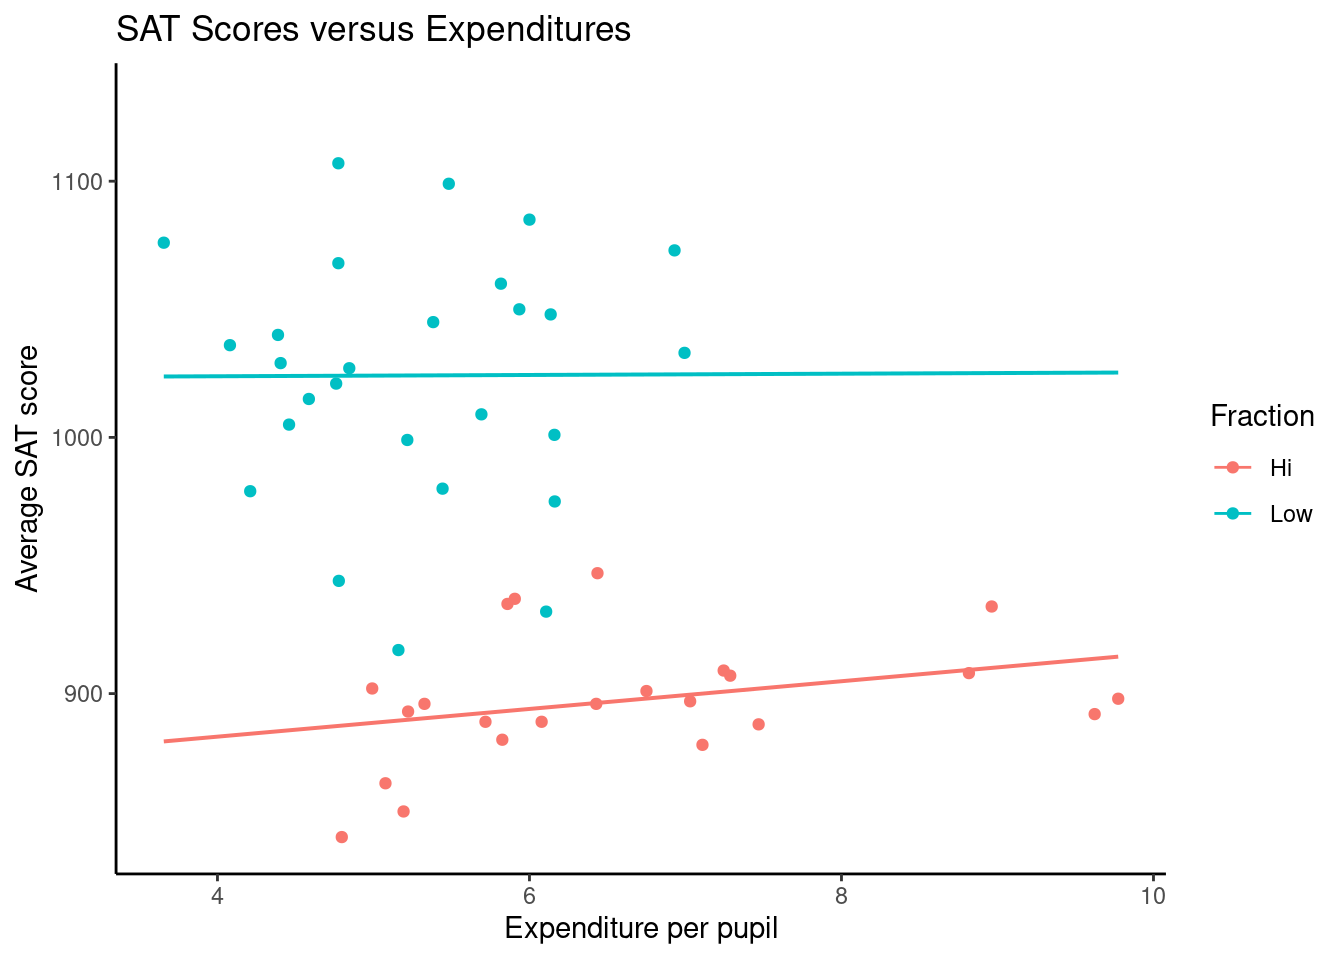
\includegraphics{04-Studies_files/figure-latex/conditional-fig-1.pdf}
\caption{\label{fig:conditional-fig}Average SAT score versus expenditure per pupil; broken down by level of participation.}
\end{figure}

Once we account for the fraction of students taking the SAT, the relationship between expenditures and SAT scores changes.

In the same way, the \texttt{county} data set is an observational study with confounding variables, and its data cannot easily be used to make causal conclusions.

\begin{quote}
\textbf{Exercise}:\\
Figure \ref{fig:homeown2-fig} shows a negative association between the homeownership rate and the percentage of multi-unit structures in a county. However, it is unreasonable to conclude that there is a causal relationship between the two variables. Suggest one or more other variables that might explain the relationship in the Figure \ref{fig:homeown2-fig}.\footnote{Answers will vary. Population density may be important. If a county is very dense, then a larger fraction of residents may live in multi-unit structures. Additionally, the high density may contribute to increases in property value, making homeownership infeasible for many residents.}
\end{quote}

\begin{figure}
\centering
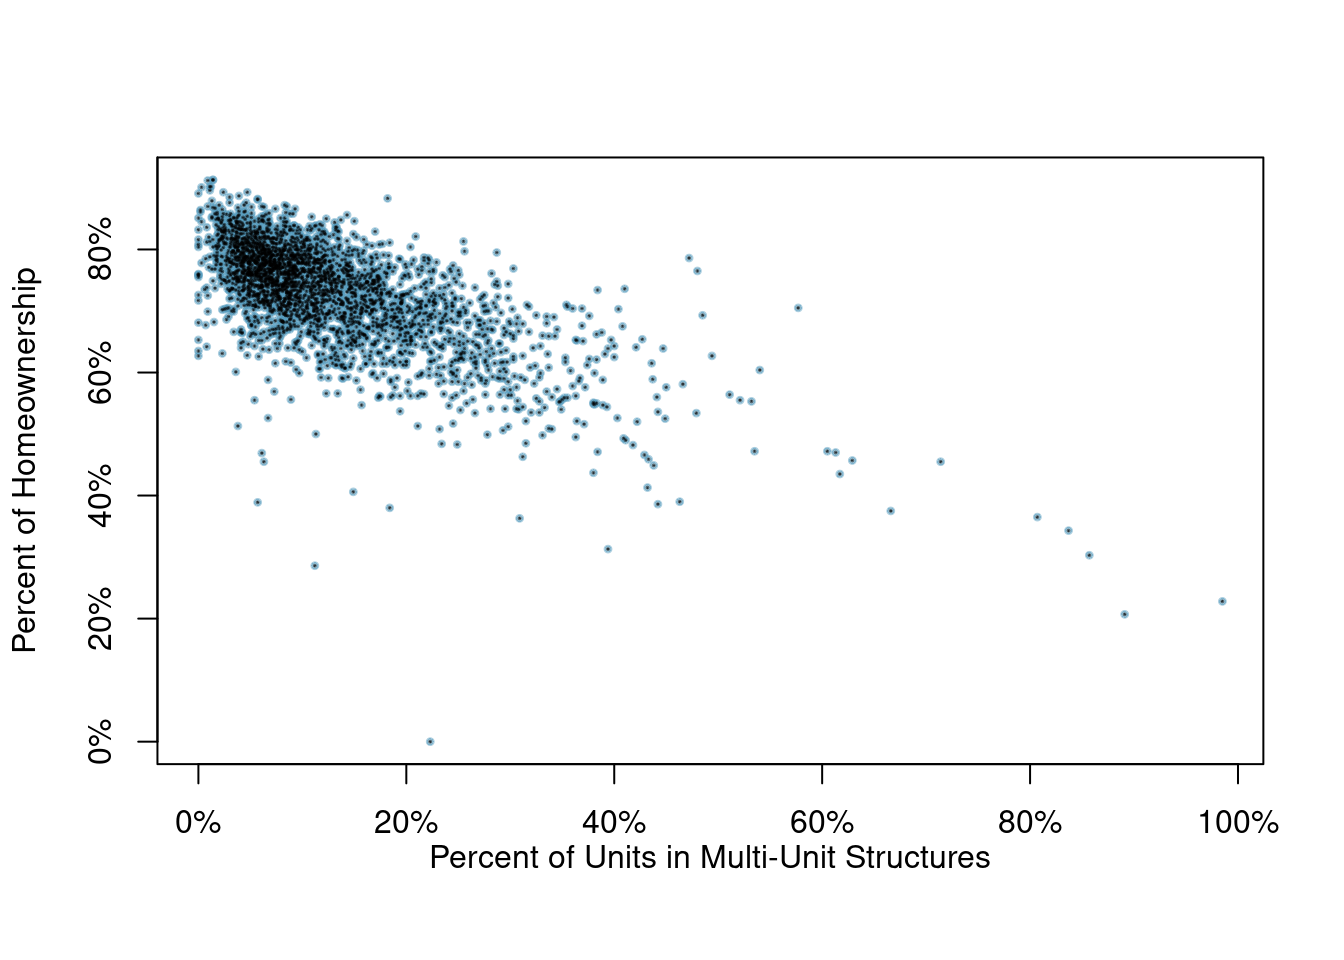
\includegraphics{04-Studies_files/figure-latex/homeown2-fig-1.pdf}
\caption{\label{fig:homeown2-fig}A scatterplot of the homeownership rate versus the percent of units that are in multi-unit structures for all 3,143 counties.}
\end{figure}

Observational studies come in two forms: prospective and retrospective studies. A \textbf{prospective study} identifies individuals and collects information as events unfold. For instance, medical researchers may identify and follow a group of similar individuals over many years to assess the possible influences of behavior on cancer risk. One example of such a study is The Nurses Health Study, started in 1976 and expanded in 1989.\footnote{\url{http://www.channing.harvard.edu/nhs/}} This prospective study recruits registered nurses and then collects data from them using questionnaires.

\textbf{Retrospective studies} collect data after events have taken place; e.g.~researchers may review past events in medical records. Some data sets, such as \texttt{county}, may contain both prospectively- and retrospectively-collected variables. Local governments prospectively collect some variables as events unfolded (e.g.~retail sales) while the federal government retrospectively collected others during the 2010 census (e.g.~county population).

\hypertarget{three-sampling-methods}{%
\subsection{Three sampling methods}\label{three-sampling-methods}}

Almost all statistical methods are based on the notion of implied randomness. If observational data are not collected in a random framework from a population, results from these statistical methods are not reliable. Here we consider three random sampling techniques: simple, stratified, and cluster sampling. Figures \ref{fig:simprand-fig} , \ref{fig:stratsamp2-fig} , and \ref{fig:clussamp4-fig} provides a graphical representation of these techniques.

\begin{figure}
\centering
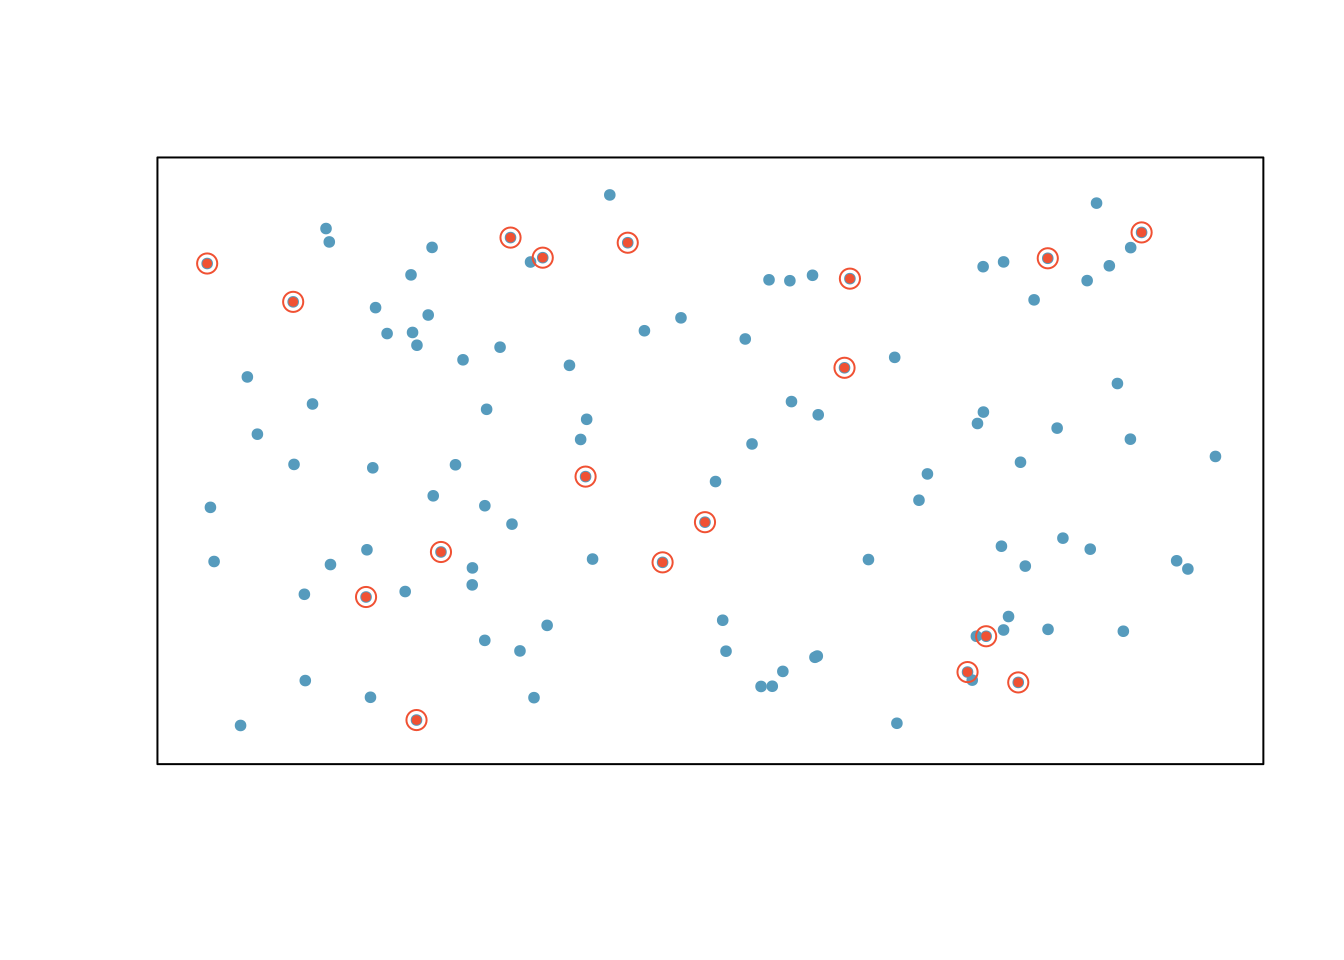
\includegraphics{04-Studies_files/figure-latex/simprand-fig-1.pdf}
\caption{\label{fig:simprand-fig}Examples of simple random sampling. In this figure, simple random sampling was used to randomly select the 18 cases.}
\end{figure}

\begin{figure}
\centering
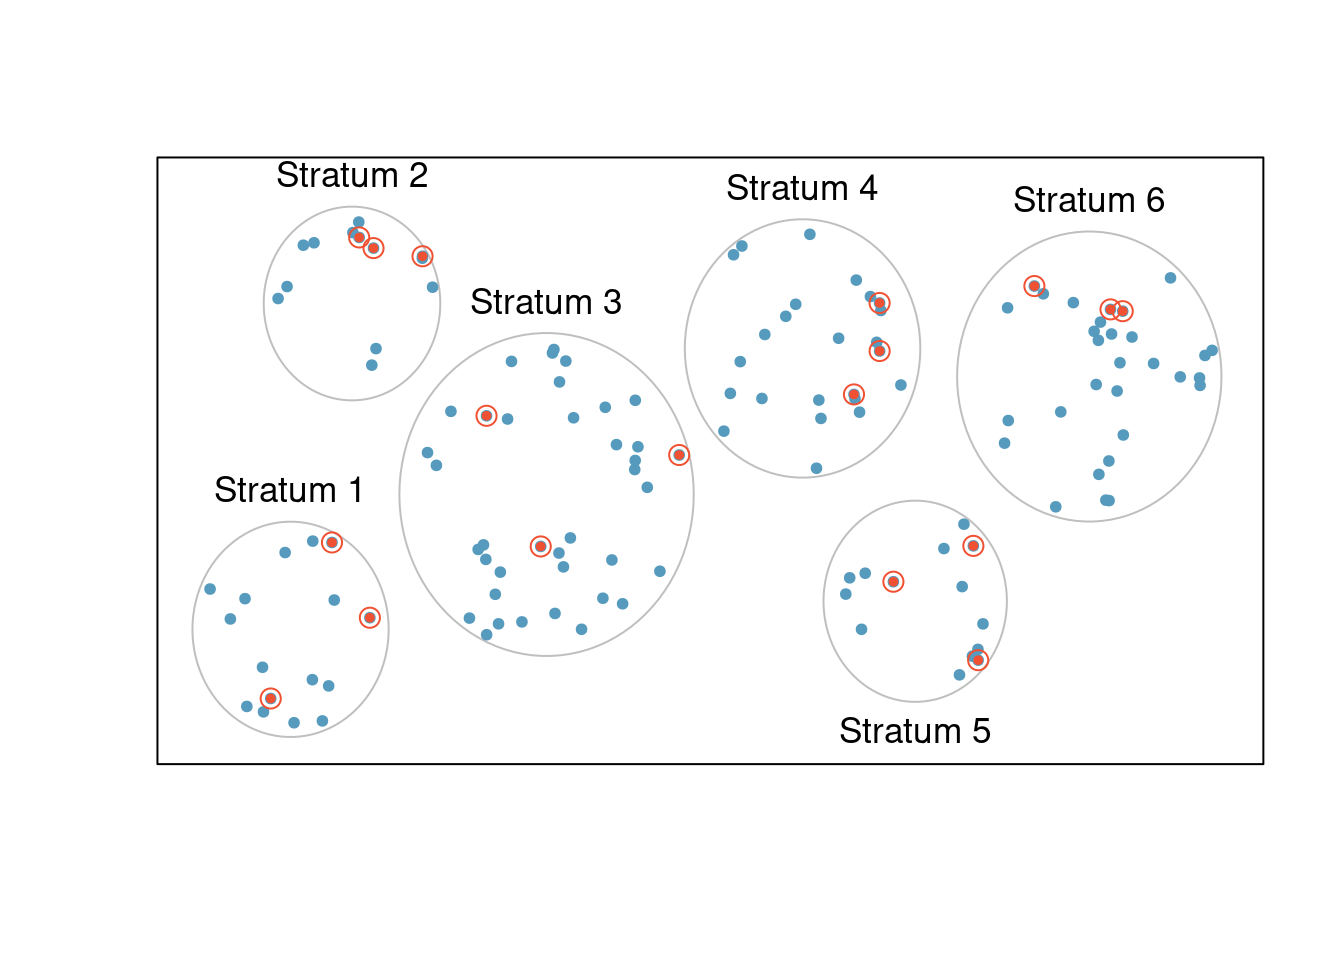
\includegraphics{04-Studies_files/figure-latex/stratsamp2-fig-1.pdf}
\caption{\label{fig:stratsamp2-fig}In this figure, stratified sampling was used: cases were grouped into strata, and then simple random sampling was employed within each stratum.}
\end{figure}

\begin{figure}
\centering
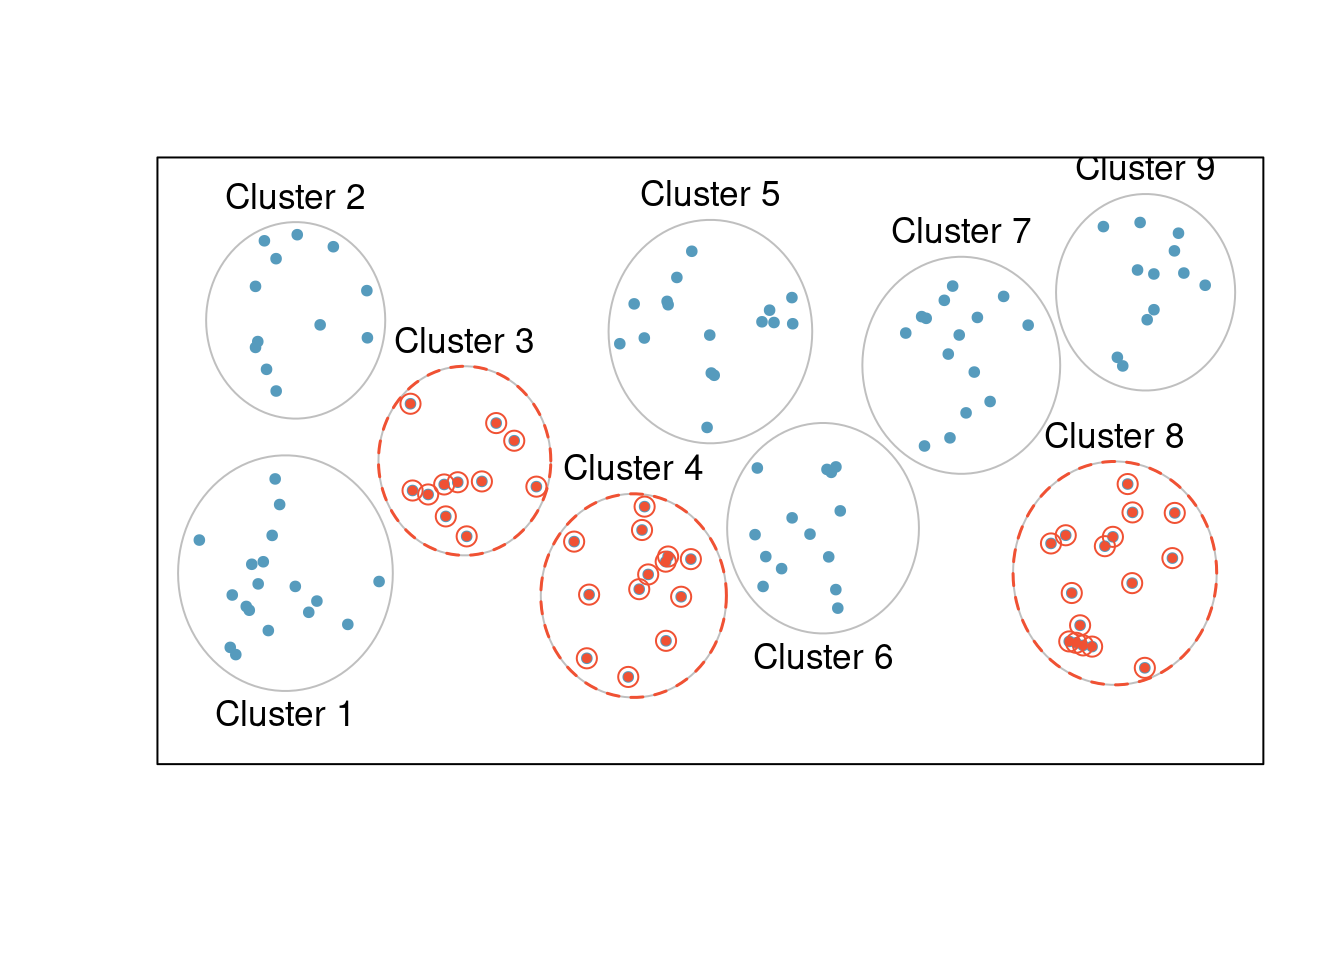
\includegraphics{04-Studies_files/figure-latex/clussamp4-fig-1.pdf}
\caption{\label{fig:clussamp4-fig}In this figure, cluster sampling was used, where data were binned into nine clusters, and three of the clusters were randomly selected.}
\end{figure}

\textbf{Simple random sampling} is probably the most intuitive form of random sampling. Consider the salaries of Major League Baseball (MLB) players, where each player is a member of one of the league's 30 teams. To take a simple random sample of 120 baseball players and their salaries from the 2010 season, we could write the names of that season's 828 players onto slips of paper, drop the slips into a bucket, shake the bucket around until we are sure the names are all mixed up, then draw out slips until we have the sample of 120 players. In general, a sample is referred to as ``simple random'\,' if each case in the population has an equal chance of being included in the final sample \emph{and} knowing that a case is included in a sample does not provide useful information about which other cases are included.

\textbf{Stratified sampling} is a divide-and-conquer sampling strategy. The population is divided into groups called \textbf{strata}. The strata are chosen so that similar cases are grouped together, then a second sampling method, usually simple random sampling, is employed within each stratum. In the baseball salary example, the teams could represent the strata; some teams have a lot more money (we're looking at you, Yankees). Then we might randomly sample 4 players from each team for a total of 120 players.

Stratified sampling is especially useful when the cases in each stratum are very similar with respect to the outcome of interest. The downside is that analyzing data from a stratified sample is a more complex task than analyzing data from a simple random sample. The analysis methods introduced in this course would need to be extended to analyze data collected using stratified sampling.

\begin{quote}
\textbf{Example}:\\
Why would it be good for cases within each stratum to be very similar?\footnote{We might get a more stable estimate for the subpopulation in a stratum if the cases are very similar. These improved estimates for each subpopulation will help us build a reliable estimate for the full population.}
\end{quote}

In \textbf{cluster sampling}, we group observations into clusters, then randomly sample some of the clusters. Sometimes cluster sampling can be a more economical technique than the alternatives. Also, unlike stratified sampling, cluster sampling is most helpful when there is a lot of case-to-case variability within a cluster but the clusters themselves don't look very different from one another. For example, if neighborhoods represented clusters, then this sampling method works best when the neighborhoods are very diverse. A downside of cluster sampling is that more advanced analysis techniques are typically required, though the methods in this course can be extended to handle such data.

\begin{quote}
\textbf{Example}:\\
Suppose we are interested in estimating the malaria rate in a densely tropical portion of rural Indonesia. We learn that there are 30 villages in that part of the Indonesian jungle, each more or less similar to the next. What sampling method should be employed?\footnote{A simple random sample would likely draw individuals from all 30 villages, which could make data collection extremely expensive. Stratified sampling would be a challenge since it is unclear how we would build strata of similar individuals. However, cluster sampling seems like a very good idea. We might randomly select a small number of villages. This would probably reduce our data collection costs substantially in comparison to a simple random sample and would still give us helpful information.}
\end{quote}

Another technique called \textbf{multistage sampling} is similar to cluster sampling, except that we take a simple random sample within each selected cluster. For instance, if we sampled neighborhoods using cluster sampling, we would next sample a subset of homes within each selected neighborhood if we were using multistage sampling.

\hypertarget{experiments}{%
\subsection{Experiments}\label{experiments}}

Studies where the researchers assign treatments to cases are called \textbf{experiments}. When this assignment includes randomization, e.g.~using a coin flip to decide which treatment a patient receives, it is called a \textbf{randomized experiment}. Randomized experiments are fundamentally important when trying to show a causal connection between two variables.

\hypertarget{principles-of-experimental-design}{%
\subsubsection{Principles of experimental design}\label{principles-of-experimental-design}}

Randomized experiments are generally built on four principles.

\begin{enumerate}
\def\labelenumi{\arabic{enumi}.}
\item
  \textbf{Controlling}. Researchers assign treatments to cases, and they do their best to \textbf{control} any other differences in the groups. For example, when patients take a drug in pill form, some patients take the pill with only a sip of water while others may have it with an entire glass of water. To control for the effect of water consumption, a doctor may ask all patients to drink a 12 ounce glass of water with the pill.
\item
  \textbf{Randomization}. Researchers randomize patients into treatment groups to account for variables that cannot be controlled. For example, some patients may be more susceptible to a disease than others due to their dietary habits. Randomizing patients into the treatment or control group helps even out such differences, and it also prevents accidental bias from entering the study.
\item
  \textbf{Replication}. The more cases researchers observe, the more accurately they can estimate the effect of the explanatory variable on the response. In a single study, we \textbf{replicate} by collecting a sufficiently large sample. Additionally, a group of scientists may replicate an entire study to verify an earlier finding. You replicate to the level of variability you want to estimate. For example, in flight test, we can run the same flight conditions again to get a replicate; however, if the same plane and pilot are being used, the replicate is not getting the pilot-to-pilot or the plane-to-plane variability.
\item
  \textbf{Blocking}. Researchers sometimes know or suspect that variables, other than the treatment, influence the response. Under these circumstances, they may first group individuals based on this variable and then randomize cases within each block to the treatment groups. This strategy is often referred to as \textbf{blocking}. For instance, if we are looking at the effect of a drug on heart attacks, we might first split patients into low-risk and high-risk \textbf{blocks}, then randomly assign half the patients from each block to the control group and the other half to the treatment group, as shown in Figure \ref{fig:exp4-fig}. This strategy ensures each treatment group has an equal number of low-risk and high-risk patients.
\end{enumerate}

\begin{figure}
\centering
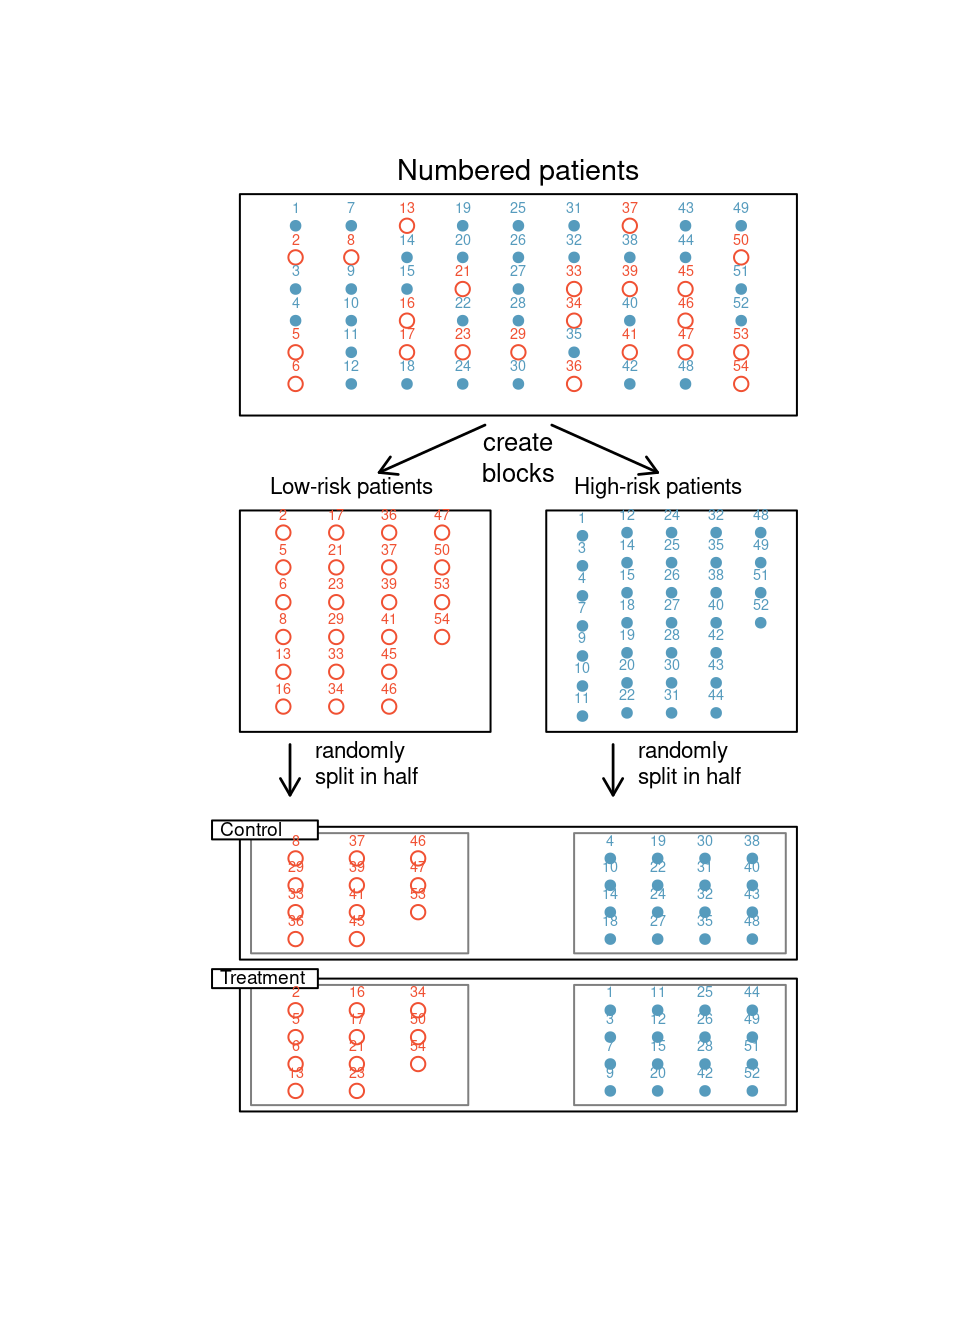
\includegraphics{04-Studies_files/figure-latex/exp4-fig-1.pdf}
\caption{\label{fig:exp4-fig}Blocking using a variable depicting patient risk. Patients are first divided into low-risk and high-risk blocks, then each block is evenly divided into the treatment groups using randomization. This strategy ensures an equal representation of patients in each treatment group from both the low-risk and high-risk categories.}
\end{figure}

It is important to incorporate the first three experimental design principles into any study, and this course describes methods for analyzing data from such experiments. Blocking is a slightly more advanced technique, and statistical methods in this course may be extended to analyze data collected using blocking. Math 359 is an entire course devoted to the design and analysis of experiments.

\hypertarget{reducing-bias-in-human-experiments}{%
\subsubsection{Reducing bias in human experiments}\label{reducing-bias-in-human-experiments}}

Randomized experiments are the gold standard for data collection, but they do not ensure an unbiased perspective into the cause and effect relationships in all cases. Human studies are perfect examples where bias can unintentionally arise. Here we reconsider a study where a new drug was used to treat heart attack patients.\footnote{Anturane Reinfarction Trial Research Group. 1980. Sulfinpyrazone in the prevention of sudden death after myocardial infarction. New England Journal of Medicine 302(5):250-256.} In particular, researchers wanted to know if the drug reduced deaths in patients.

These researchers designed a randomized experiment because they wanted to draw causal conclusions about the drug's effect. Study volunteers\footnote{Human subjects are often called \textbf{patients}, \textbf{volunteers}, or \textbf{study participants}.} were randomly placed into two study groups. One group, the \textbf{treatment group}, received the drug. The other group, called the \textbf{control group}, did not receive any drug treatment.

Put yourself in the place of a person in the study. If you are in the treatment group, you are given a fancy new drug that you anticipate will help you. On the other hand, a person in the other group doesn't receive the drug and sits idly, hoping her participation doesn't increase her risk of death. These perspectives suggest there are actually two effects: the one of interest is the effectiveness of the drug, and the second is an emotional effect that is difficult to quantify.

Researchers aren't usually interested in the emotional effect, which might bias the study. To circumvent this problem, researchers do not want patients to know which group they are in. When researchers keep the patients uninformed about their treatment, the study is said to be \textbf{blind}. But there is one problem: if a patient doesn't receive a treatment, she will know she is in the control group. The solution to this problem is to give fake treatments to patients in the control group. A fake treatment is called a \textbf{placebo}, and an effective placebo is the key to making a study truly blind. A classic example of a placebo is a sugar pill that is made to look like the actual treatment pill. Often times, a placebo results in a slight but real improvement in patients. This effect has been dubbed the \textbf{placebo effect}.

The patients are not the only ones who should be blinded: doctors and researchers can accidentally bias a study. When a doctor knows a patient has been given the real treatment, she might inadvertently give that patient more attention or care than a patient that she knows is on the placebo. To guard against this bias, which again has been found to have a measurable effect in some instances, most modern studies employ a \textbf{double-blind} setup where doctors or researchers who interact with patients are, just like the patients, unaware of who is or is not receiving the treatment.\footnote{There are always some researchers in the study who do know which patients are receiving which treatment. However, they do not interact with the study's patients and do not tell the blinded health care professionals who is receiving which treatment.}

\begin{quote}
\textbf{Exercise}:\\
Look back to the stent study in the first lesson where researchers were testing whether stents were effective at reducing strokes in at-risk patients. Is this an experiment? Was the study blinded? Was it double-blinded?\footnote{The researchers assigned the patients into their treatment groups, so this study was an experiment. However, the patients could distinguish what treatment they received, so this study was not blind. The study could not be double-blind since it was not blind.}
\end{quote}

\hypertarget{homework-problems-3}{%
\section{Homework Problems}\label{homework-problems-3}}

\begin{enumerate}
\def\labelenumi{\arabic{enumi}.}
\tightlist
\item
  \textbf{Propose a sampling strategy}. A large college class has 160 students. All 160 students attend the lectures together, but the students are divided into 4 groups, each of 40 students, for lab sections administered by different teaching assistants. The professor wants to conduct a survey about how satisfied the students are with the course, and he believes that the lab section a student is in might affect the student's overall satisfaction with the course.
\end{enumerate}

\begin{enumerate}
\def\labelenumi{\alph{enumi}.}
\tightlist
\item
  What type of study is this?\\
\item
  Suggest a sampling strategy for carrying out this study.
\end{enumerate}

\begin{enumerate}
\def\labelenumi{\arabic{enumi}.}
\setcounter{enumi}{1}
\tightlist
\item
  \textbf{Flawed reasoning}. Identify the flaw in reasoning in the following scenarios. Explain what the individuals in the study should have done differently if they wanted to make such strong conclusions.
\end{enumerate}

\begin{enumerate}
\def\labelenumi{\alph{enumi}.}
\tightlist
\item
  Students at an elementary school are given a questionnaire that they are required to return after their parents have completed it. One of the questions asked is, \emph{Do you find that your work schedule makes it difficult for you to spend time with your kids after school?} Of the parents who replied, 85\% said \emph{no}. Based on these results, the school officials conclude that a great majority of the parents have no difficulty spending time with their kids after school.\\
\item
  A survey is conducted on a simple random sample of 1,000 women who recently gave birth, asking them about whether or not they smoked during pregnancy. A follow-up survey asking if the children have respiratory problems is conducted 3 years later, however, only 567 of these women are reached at the same address. The researcher reports that these 567 women are representative of all mothers.
\end{enumerate}

\begin{enumerate}
\def\labelenumi{\arabic{enumi}.}
\setcounter{enumi}{2}
\tightlist
\item
  \textbf{Sampling strategies}. A Math 377 student who is curious about the relationship between the amount of time students spend on social networking sites and their performance at school decides to conduct a survey. Four research strategies for collecting data are described below. In each, name the sampling method proposed and any bias you might expect.
\end{enumerate}

\begin{enumerate}
\def\labelenumi{\alph{enumi}.}
\tightlist
\item
  He randomly samples 40 students from the study's population, gives them the survey, asks them to fill it out and bring it back the next day.\\
\item
  He gives out the survey only to his friends, and makes sure each one of them fills out the survey.\\
\item
  He posts a link to an online survey on his Facebook wall and asks his friends to fill out the survey.\\
\item
  He stands outside the QRC and asks every third person that walks out the door to fill out the survey.
\end{enumerate}

\pagebreak

\begin{enumerate}
\def\labelenumi{\arabic{enumi}.}
\setcounter{enumi}{3}
\tightlist
\item
  \textbf{Vitamin supplements}. In order to assess the effectiveness of taking large doses of vitamin C in reducing the duration of the common cold, researchers recruited 400 healthy volunteers from staff and students at a university. A quarter of the patients were assigned a placebo, and the rest were evenly divided between 1g Vitamin C, 3g Vitamin C, or 3g Vitamin C plus additives to be taken at onset of a cold for the following two days. All tablets had identical appearance and packaging. The nurses who handed the prescribed pills to the patients knew which patient received which treatment, but the researchers assessing the patients when they were sick did not. No significant differences were observed in any measure of cold duration or severity between the four medication groups, and the placebo group had the shortest duration of symptoms.
\end{enumerate}

\begin{enumerate}
\def\labelenumi{\alph{enumi}.}
\tightlist
\item
  Was this an experiment or an observational study? Why?\\
\item
  What are the explanatory and response variables in this study?\\
\item
  Were the patients blinded to their treatment?\\
\item
  Was this study double-blind?\\
\item
  Participants are ultimately able to choose whether or not to use the pills prescribed to them. We might expect that not all of them will adhere and take their pills. Does this introduce a confounding variable to the study? Explain your reasoning.
\end{enumerate}

\begin{enumerate}
\def\labelenumi{\arabic{enumi}.}
\setcounter{enumi}{4}
\tightlist
\item
  \textbf{Exercise and mental health}. A researcher is interested in the effects of exercise on mental health and she proposes the following study: Use stratified random sampling to ensure representative proportions of 18-30, 31-40 and 41-55 year olds from the population. Next, randomly assign half the subjects from each age group to exercise twice a week, and instruct the rest not to exercise. Conduct a mental health exam at the beginning and at the end of the study, and compare the results.
\end{enumerate}

\begin{enumerate}
\def\labelenumi{\alph{enumi}.}
\tightlist
\item
  What type of study is this?\\
\item
  What are the treatment and control groups in this study?\\
\item
  Does this study make use of blocking? If so, what is the blocking variable?\\
\item
  Does this study make use of blinding?\\
\item
  Comment on whether or not the results of the study can be used to establish a causal relationship between exercise and mental health, and indicate whether or not the conclusions can be generalized to the population at large.\\
\item
  Suppose you are given the task of determining if this proposed study should get funding. Would you have any reservations about the study proposal?
\end{enumerate}

\hypertarget{NUMDATA}{%
\chapter{Numerical Data}\label{NUMDATA}}

\hypertarget{objectives-4}{%
\section{Objectives}\label{objectives-4}}

\begin{enumerate}
\def\labelenumi{\arabic{enumi})}
\tightlist
\item
  Define and use properly in context all new terminology.\\
\item
  Generate in \texttt{R} summary statistics for a numeric variable including breaking down by cases.\\
\item
  Generate in \texttt{R} appropriate graphical summaries of numerical variables.\\
\item
  Be able to interpret and explain output both graphically and numerically.
\end{enumerate}

\hypertarget{numerical-data}{%
\section{Numerical Data}\label{numerical-data}}

This lesson introduces techniques for exploring and summarizing numerical variables, and the \texttt{email50} and \texttt{mlb} data sets from the \textbf{openintro} package and a subset of \texttt{county\_complete} from \texttt{usdata} provide rich opportunities for examples. Recall that outcomes of numerical variables are numbers on which it is reasonable to perform basic arithmetic operations. For example, the \texttt{pop2010} variable, which represents the populations of counties in 2010, is numerical since we can sensibly discuss the difference or ratio of the populations in two counties. On the other hand, area codes and zip codes are not numerical.

\hypertarget{scatterplots-for-paired-data}{%
\subsection{Scatterplots for paired data}\label{scatterplots-for-paired-data}}

A \textbf{scatterplot} provides a case-by-case view of data for two numerical variables. In Figure \ref{fig:scat5-fig}, we again present a scatterplot used to examine how federal spending and poverty were related in the \texttt{county} data set.

\begin{figure}
\centering
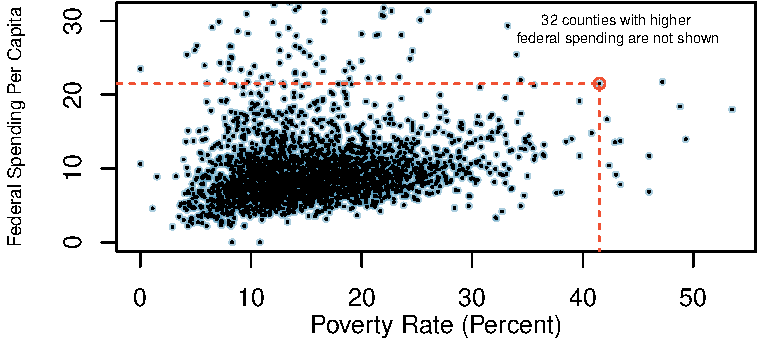
\includegraphics{05-Numerical-Data_files/figure-latex/scat5-fig-1.pdf}
\caption{\label{fig:scat5-fig}A scatterplot showing fed\_spend against poverty. Owsley County of Kentucky, with a poverty rate of 41.5\% and federal spending of \$21.50 per capita, is highlighted.}
\end{figure}

Another scatterplot is shown in Figure \ref{fig:scat52-fig}, comparing the number of line breaks \texttt{line\_breaks} and number of characters \texttt{num\_char} in emails for the \texttt{email50} data set. In any scatterplot, each point represents a single case. Since there are 50 cases in \texttt{email50}, there are 50 points in Figure \ref{fig:scat52-fig}.

\begin{figure}
\centering
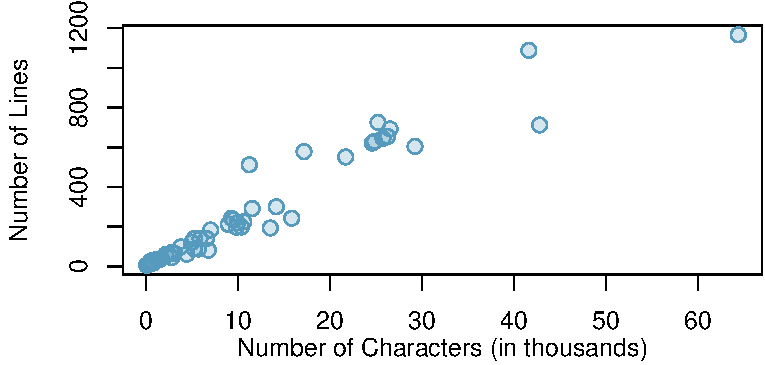
\includegraphics{05-Numerical-Data_files/figure-latex/scat52-fig-1.pdf}
\caption{\label{fig:scat52-fig}A scatterplot of \texttt{line\_breaks} versus \texttt{num\_char} for the \texttt{email50} data.}
\end{figure}

To put the number of characters in perspective, this paragraph has 357 characters. Looking at Figure \ref{fig:scat52-fig}, it seems that some emails are incredibly long! Upon further investigation, we would actually find that most of the long emails use the HTML format, which means most of the characters in those emails are used to format the email rather than provide text.

\pagebreak

\begin{quote}
\textbf{Exercise}:\\
What do scatterplots reveal about the data, and how might they be useful?\footnote{Answers may vary. Scatterplots are helpful in quickly spotting associations between variables, whether those associations represent simple or more complex relationships.}
\end{quote}

\begin{quote}
\emph{Example}:\\
Consider a new data set of 54 cars with two variables: vehicle price and weight.\footnote{Subset of data from \url{http://www.amstat.org/publications/jse/v1n1/datasets.lock.html}} A scatterplot of vehicle price versus weight is shown in Figure \ref{fig:scat53-fig}. What can be said about the relationship between these variables?
\end{quote}

\begin{figure}
\centering
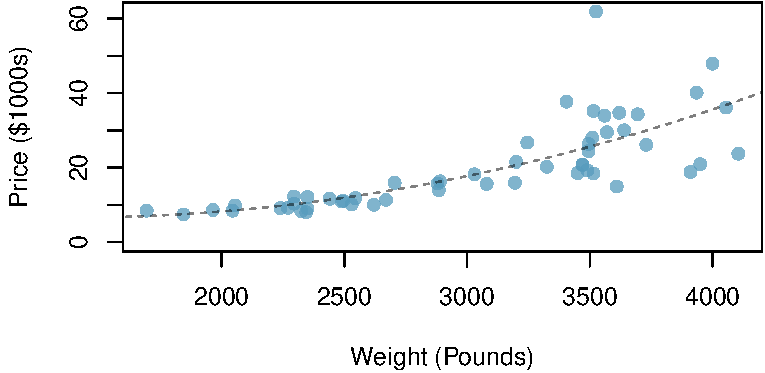
\includegraphics{05-Numerical-Data_files/figure-latex/scat53-fig-1.pdf}
\caption{\label{fig:scat53-fig}A scatterplot of \emph{price} versus \emph{weight} for 54 cars.}
\end{figure}

The relationship is evidently nonlinear, as highlighted by the dashed line. This is different from previous scatterplots we've seen which show relationships that are very linear.

\begin{quote}
\textbf{Exercise}:\\
Describe two variables that would have a horseshoe shaped association in a scatterplot.\footnote{Consider the case where your vertical axis represents something ``good'\,' and your horizontal axis represents something that is only good in moderation. Health and water consumption fit this description since water becomes toxic when consumed in excessive quantities.}
\end{quote}

\hypertarget{dot-plots-and-the-mean}{%
\subsection{Dot plots and the mean}\label{dot-plots-and-the-mean}}

Sometimes two variables are one too many: only one variable may be of interest. In these cases, a dot plot provides the most basic of displays. A \textbf{dot plot} is a one-variable scatterplot; an example using the number of characters from 50 emails is shown in Figure \ref{fig:dot5-fig}.

\begin{figure}
\centering
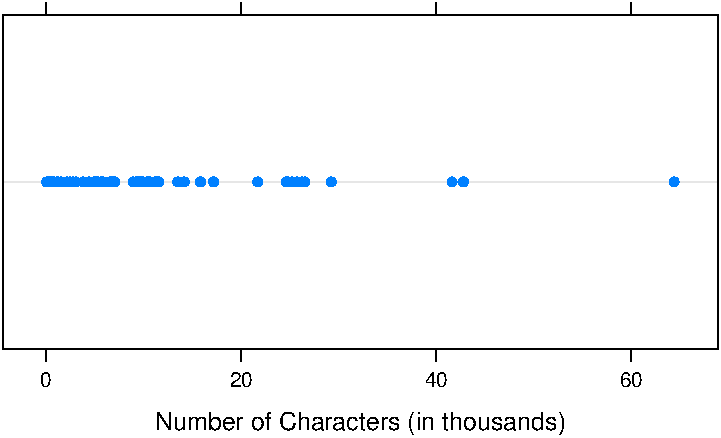
\includegraphics{05-Numerical-Data_files/figure-latex/dot5-fig-1.pdf}
\caption{\label{fig:dot5-fig}A dot plot of \texttt{num\_char} for the \texttt{email50} data set.}
\end{figure}

The \textbf{mean}, sometimes called the average, is a common way to measure the center of a \textbf{distribution} of data. To find the mean number of characters in the 50 emails, we add up all the character counts and divide by the number of emails. For computational convenience, the number of characters is listed in the thousands and rounded to the first decimal.

\[\bar{x} = \frac{21.7 + 7.0 + \cdots + 15.8}{50} = 11.6\]

The sample mean is often labeled \(\bar{x}\), and the letter \(x\) is being used as a generic placeholder for the variable of interest, \texttt{num\_char}.

\begin{quote}
\textbf{Mean}\\
The sample mean of a numerical variable is the sum of all of the observations divided by the number of observations, Equation \eqref{eq:mean5}.
\end{quote}

\begin{equation} 
  \bar{x} = \frac{x_1+x_2+\cdots+x_n}{n}
  \label{eq:mean5}
\end{equation}

where \(x_1, x_2, \dots, x_n\) represent the \(n\) observed values.

\begin{quote}
\textbf{Exercise}:\\
Examine the two equations above. What does \(x_1\) correspond to? And \(x_2\)? Can you infer a general meaning to what \(x_i\) might represent?\footnote{\(x_1\) corresponds to the number of characters in the first email in the sample (21.7, in thousands), \(x_2\) to the number of characters in the second email (7.0, in thousands), and \(x_i\) corresponds to the number of characters in the \(i^{th}\) email in the data set.}
\end{quote}

\begin{quote}
\textbf{Exercise}:\\
What was \(n\) in this sample of emails?\footnote{The sample size was \(n=50\).}
\end{quote}

The \texttt{email50} data set is a sample from a larger population of emails that were received in January and March. We could compute a mean for this population in the same way as the sample mean. However, there is a difference in notation: the population mean has a special label: \(\mu\). The symbol \(\mu\) is the Greek letter \emph{mu} and represents the average of all observations in the population. Sometimes a subscript, such as \(_x\), is used to represent which variable the population mean refers to, e.g.~\(\mu_x\).

\begin{quote}
\emph{Example}:
The average number of characters across all emails can be estimated using the sample data. Based on the sample of 50 emails, what would be a reasonable estimate of \(\mu_x\), the mean number of characters in all emails in the \texttt{email} data set? (Recall that \texttt{email50} is a sample from \texttt{email}.)
\end{quote}

The sample mean, 11.6, may provide a reasonable estimate of \(\mu_x\). While this number will not be perfect, it provides a \textbf{point estimate} of the population mean. Later in the semester, we will develop tools to characterize the accuracy of point estimates, and we will find that point estimates based on larger samples tend to be more accurate than those based on smaller samples.

\begin{quote}
\emph{Example}:\\
We might like to compute the average income per person in the US. To do so, we might first think to take the mean of the per capita incomes from the 3,143 counties in the \texttt{county} data set. What would be a better approach?
\end{quote}

The \texttt{county} data set is special in that each county actually represents many individual people. If we were to simply average across the \texttt{income} variable, we would be treating counties with 5,000 and 5,000,000 residents equally in the calculations. Instead, we should compute the total income for each county, add up all the counties' totals, and then divide by the number of people in all the counties. If we completed these steps with the \texttt{county} data, we would find that the per capita income for the US is \$27,348.43. Had we computed the \emph{simple} mean of per capita income across counties, the result would have been just \$22,504.70!

This previous example used what is called a \textbf{weighted mean}, which will be a key topic in the probability section. As a look ahead, the probability mass function gives the population proportions of each value and thus to find the population mean \(\mu\), we will use a weighted mean.

\hypertarget{histograms-and-shape}{%
\subsection{Histograms and shape}\label{histograms-and-shape}}

Dot plots show the exact value of each observation. This is useful for small data sets, but they can become hard to read with larger samples. Rather than showing the value of each observation, think of the value as belonging to a \emph{bin}. For example, in the \texttt{email50} data set, we create a table of counts for the number of cases with character counts between 0 and 5,000, then the number of cases between 5,000 and 10,000, and so on. Observations that fall on the boundary of a bin (e.g.~5,000) are allocated to the lower bin. This tabulation is shown below.

\begin{verbatim}
## 
##   (0,5]  (5,10] (10,15] (15,20] (20,25] (25,30] (30,35] (35,40] (40,45] (45,50] 
##      19      12       6       2       3       5       0       0       2       0 
## (50,55] (55,60] (60,65] 
##       0       0       1
\end{verbatim}

These binned counts are plotted as bars in Figure \ref{fig:hist5-fig} into what is called a \textbf{histogram}.

\begin{figure}
\centering
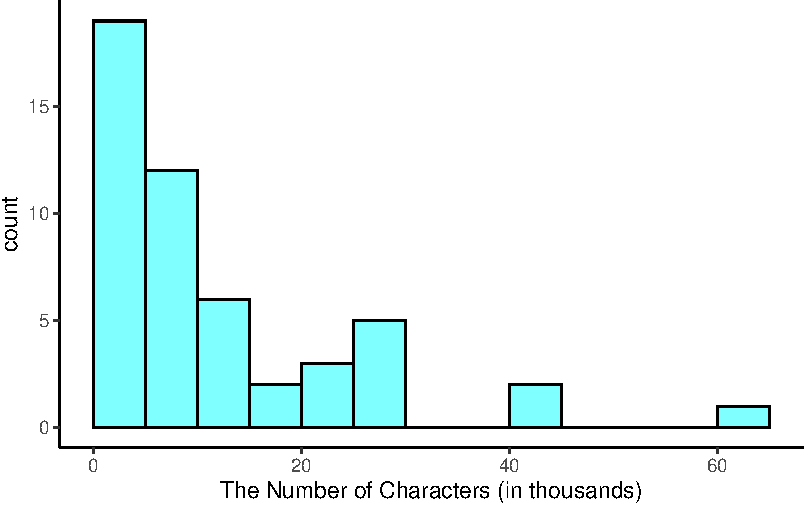
\includegraphics{05-Numerical-Data_files/figure-latex/hist5-fig-1.pdf}
\caption{\label{fig:hist5-fig}A histogram of \texttt{num\_char}. This distribution is very strongly skewed to the right.}
\end{figure}

Histograms provide a view of the \textbf{data density}. Higher bars represent where the data are relatively more dense. For instance, there are many more emails between 0 and 10,000 characters than emails between 10,000 and 20,000 characters in the data set. The bars make it easy to see how the density of the data changes relative to the number of characters.

Histograms are especially convenient for describing the shape of the data distribution. Figure \ref{fig:hist5-fig} shows that most emails have a relatively small number of characters, while fewer emails have a very large number of characters. When data trail off to the right in this way and have a longer right \textbf{tail}, the shape is said to be \textbf{right skewed}.\footnote{Other ways to describe data that are skewed to the right: \textbf{skewed to the right}, \textbf{skewed to the high end}, or \textbf{skewed to the positive end}.}

Data sets with the reverse characteristic -- a long, thin tail to the left -- are said to be \textbf{left skewed}. We also say that such a distribution has a long left tail. Data sets that show roughly equal trailing off in both directions are called \textbf{symmetric}.

\begin{quote}
\textbf{Long tails to identify skew}\\
When data trail off in one direction, the distribution has a \textbf{long tail}. If a distribution has a long left tail, it is left skewed. If a distribution has a long right tail, it is right skewed.
\end{quote}

\begin{quote}
\textbf{Exercise}:\\
Take a look at the dot plot above, Figure \ref{fig:dot5-fig}. Can you see the skew in the data? Is it easier to see the skew in this histogram or the dot plots?\footnote{The skew is visible in all both plots, though the dot plot is the least useful.}
\end{quote}

\begin{quote}
\textbf{Exercise}:\\
Besides the mean, what can you see in the dot plot that you cannot see in the histogram?\footnote{Character counts for individual emails.}
\end{quote}

\hypertarget{making-our-own-histogram}{%
\subsubsection{Making our own histogram}\label{making-our-own-histogram}}

Let's take some time to make a simple histogram. We will use the \textbf{ggformula} package which is a wrapper for the \textbf{ggplot} package.

Here are two questions:\\
\emph{What do we want \texttt{R} to do?} and\\
\emph{What must we give \texttt{R} for it to do this?}

We want \texttt{R} to make a histogram. In \texttt{ggformula} the plots have the form \texttt{gf\_XXXX} so we will use the \texttt{gf\_histogram}. To find options and more information type:

\begin{verbatim}
?gf_histogram
\end{verbatim}

To start we just have to give the formulas and data to \texttt{R}.

\begin{Shaded}
\begin{Highlighting}[]
\FunctionTok{gf\_histogram}\NormalTok{(}\SpecialCharTok{\textasciitilde{}}\NormalTok{num\_char,}\AttributeTok{data=}\NormalTok{email50)}
\end{Highlighting}
\end{Shaded}

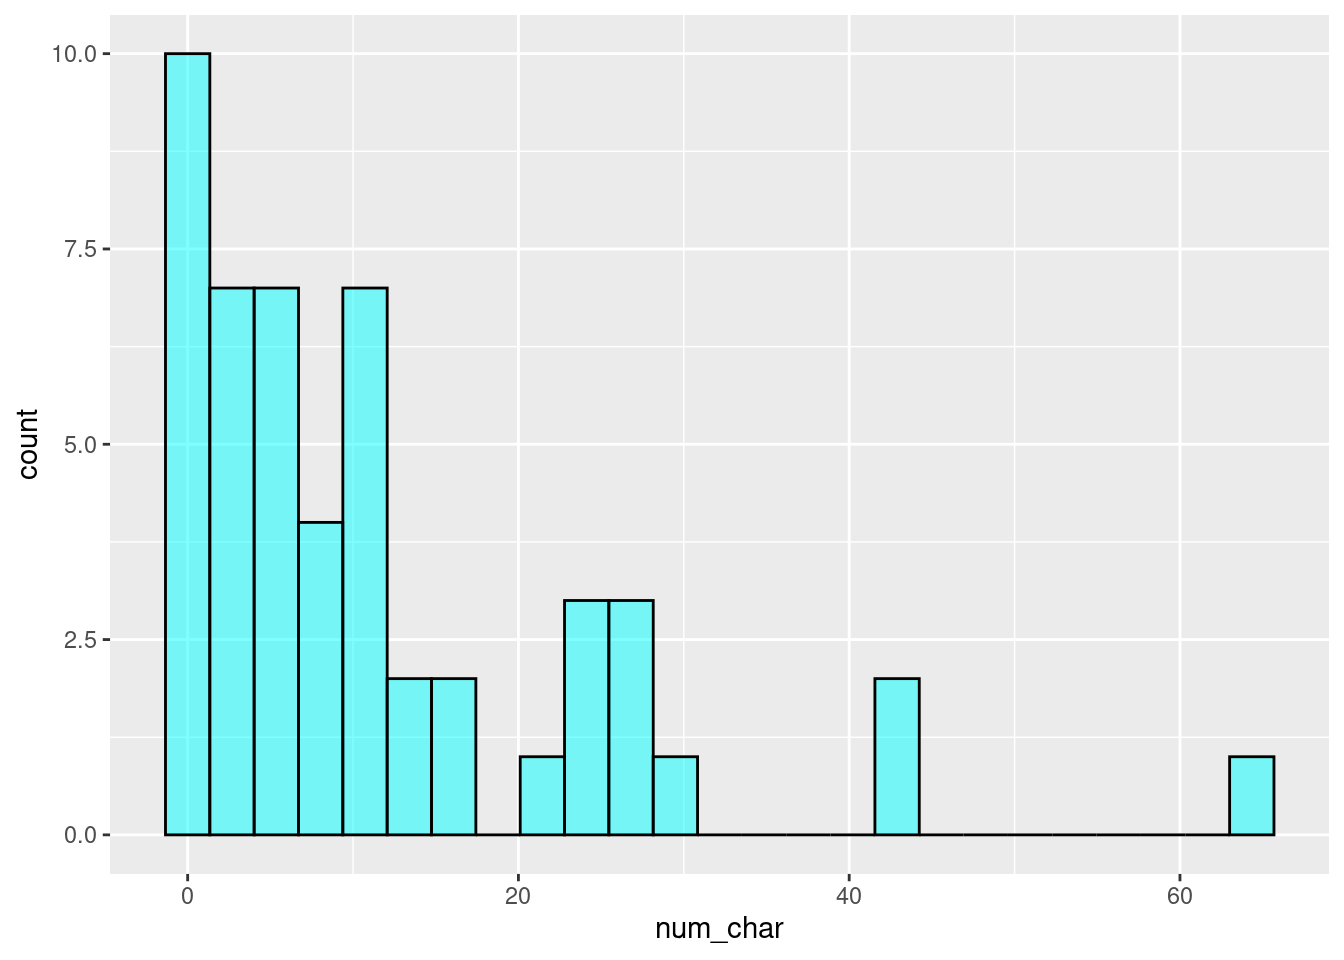
\includegraphics{05-Numerical-Data_files/figure-latex/unnamed-chunk-4-1.pdf}

\begin{quote}
\textbf{Exercise}:\\
Look at the help menu for \texttt{gf\_histogram} and change the x-axis label, change the bin width to 5, and have the left bin start at 0.
\end{quote}

Here is the code for the exercise

\begin{verbatim}
email50 %>%
   gf_histogram(~num_char,binwidth = 5,boundary=0,
   xlab="The Number of Characters (in thousands)") %>%
   gf_theme(theme_classic())
\end{verbatim}

In addition to looking at whether a distribution is skewed or symmetric, histograms can be used to identify modes. A \textbf{mode} is represented by a prominent peak in the distribution.\footnote{Another definition of mode, which is not typically used in statistics, is the value with the most occurrences. It is common to have \emph{no} observations with the same value in a data set, which makes this other definition useless for many real data sets.} There is only one prominent peak in the histogram of \texttt{num\_char}.

Figure \ref{fig:histmulti-fig} show histograms that have one, two, or three prominent peaks. Such distributions are called \textbf{unimodal}, \textbf{bimodal}, and \textbf{multimodal}, respectively. Any distribution with more than 2 prominent peaks is called multimodal. Notice that there was one prominent peak in the unimodal distribution with a second less prominent peak that was not counted since it only differs from its neighboring bins by a few observations.

\begin{figure}
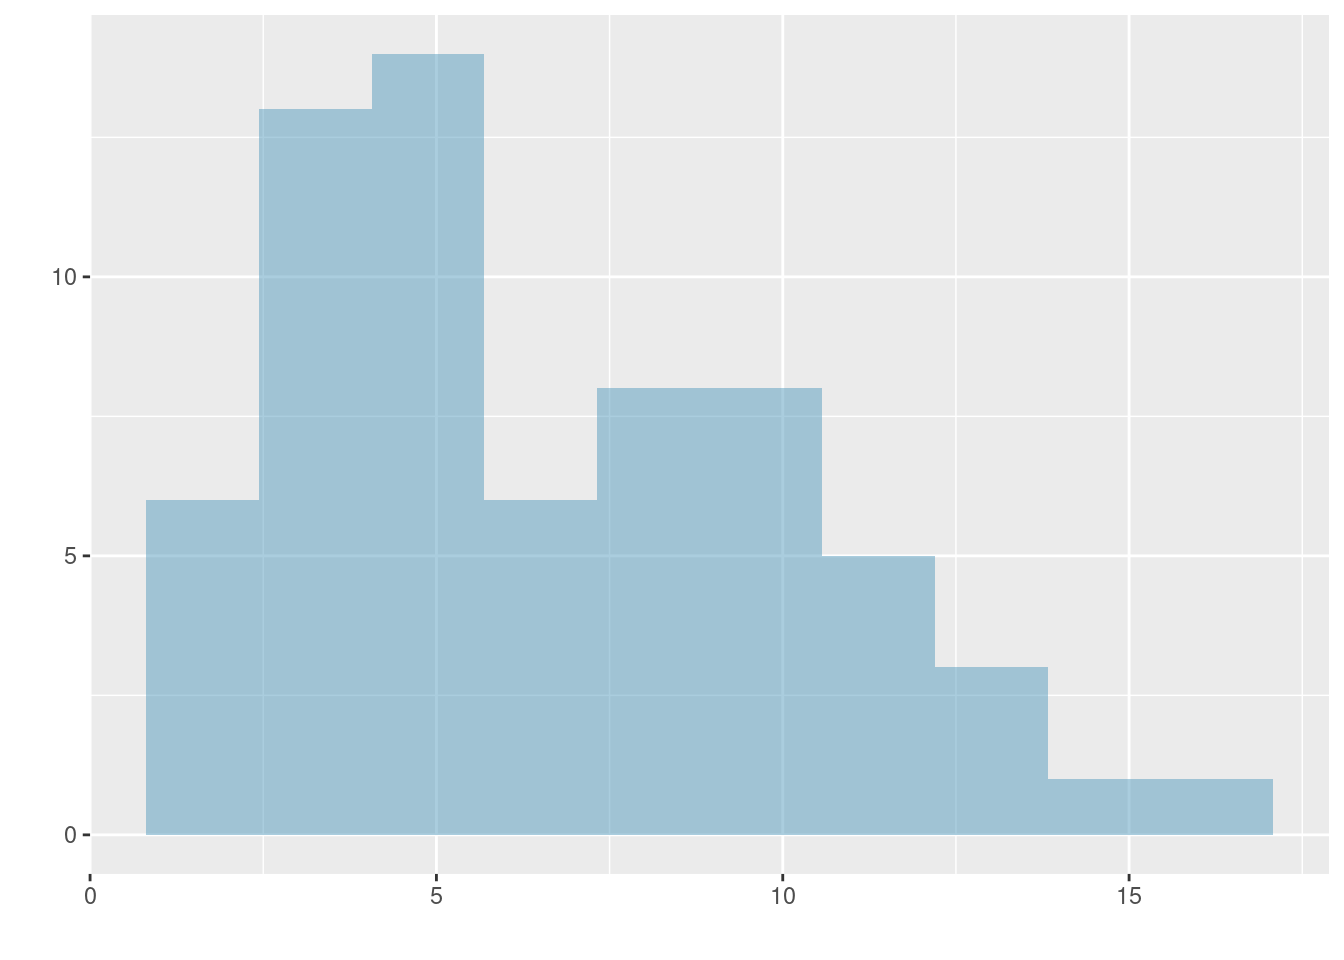
\includegraphics[width=0.33\linewidth]{05-Numerical-Data_files/figure-latex/histmulti-fig-1} 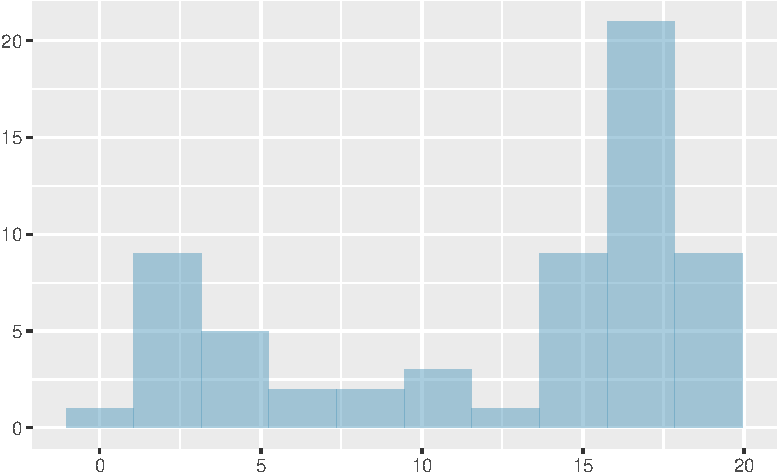
\includegraphics[width=0.33\linewidth]{05-Numerical-Data_files/figure-latex/histmulti-fig-2} 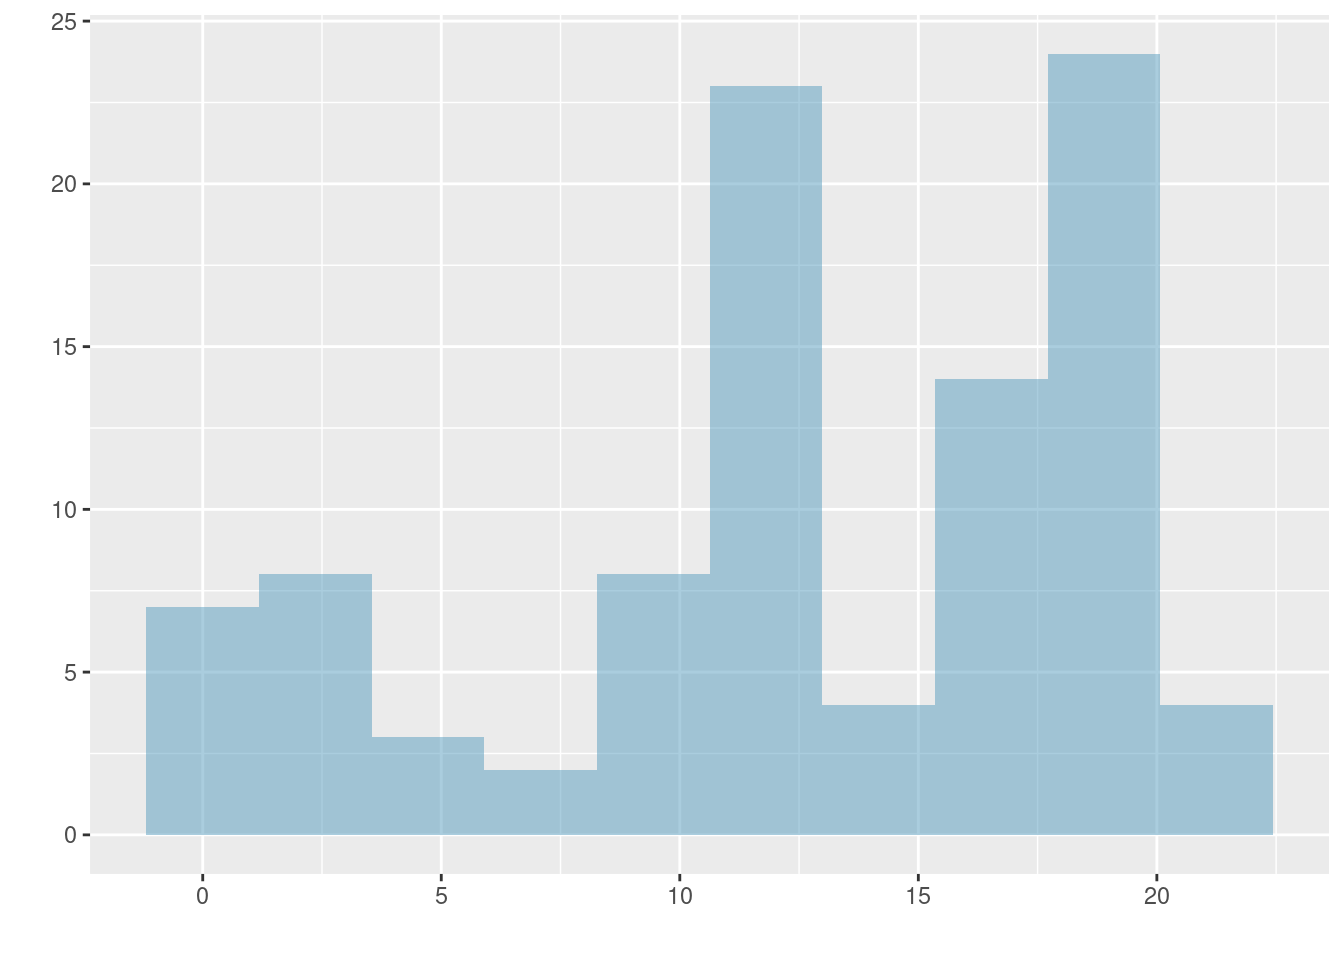
\includegraphics[width=0.33\linewidth]{05-Numerical-Data_files/figure-latex/histmulti-fig-3} \caption{Histograms that demonstrate unimodal, bimodal, and multimodal data.}\label{fig:histmulti-fig}
\end{figure}

\begin{quote}
\textbf{Exercise}:\\
Height measurements of young students and adult teachers at a K-3 elementary school were taken. How many modes would you anticipate in this height data set?\footnote{There might be two height groups visible in the data set: one of the students and one of the adults. That is, the data are probably bimodal. But it could be multimodal because within each group we may be able to see a difference in males and females.}
\end{quote}

\begin{quote}
\textbf{Looking for modes}\\
Looking for modes isn't about finding a clear and correct answer about the number of modes in a distribution, which is why \textbf{prominent} is not rigorously defined in these notes. The important part of this examination is to better understand your data and how it might be structured.
\end{quote}

\hypertarget{variance-and-standard-deviation}{%
\subsection{Variance and standard deviation}\label{variance-and-standard-deviation}}

The mean is used to describe the center of a data set, but the \emph{variability} in the data is also important. Here, we introduce two measures of variability: the \textbf{variance} and the \textbf{standard deviation}. Both of these are very useful in data analysis, even though the formulas are a bit tedious to calculate by hand. The standard deviation is the easier of the two to conceptually understand, and it roughly describes how far away the typical observation is from the mean. Equation \eqref{eq:var5} is the equation for sample variance. We will demonstrate it with data so that the notation is easier to understand.

\begin{equation} 
  s^2 = \sum_{i=1}^{n}\frac{(x_i-\bar{x})^2}{n-1}=\frac{(x_1-\bar{x})^2 + (x_2-\bar{x})^2 + (x_3-\bar{x})^2 + \cdots + (x_n-\bar{x})^2}{n-1}
  \label{eq:var5}
\end{equation}

where \(x_1, x_2, \dots, x_n\) represent the \(n\) observed values.

We call the distance of an observation from its mean its \textbf{deviation}. Below are the deviations for the \(1^{st}\), \(2^{nd}\), \(3^{rd}\), and \(50^{th}\) observations in the \texttt{num\_char} variable. For computational convenience, the number of characters is listed in the thousands and rounded to the first decimal.

\[
\begin{aligned}
x_1^{}-\bar{x} &= 21.7 - 11.6 = 10.1 \hspace{5mm}\text{ } \\
x_2^{}-\bar{x} &= 7.0 - 11.6 = -4.6 \\
x_3^{}-\bar{x} &= 0.6 - 11.6 = -11.0 \\
            &\ \vdots \\
x_{50}^{}-\bar{x} &= 15.8 - 11.6 = 4.2
\end{aligned}
\]

If we square these deviations and then take an average, the result is equal to the \textbf{sample variance}, denoted by \(s_{}^2\):
\[
\begin{aligned}
s_{}^2 &= \frac{10.1_{}^2 + (-4.6)_{}^2 + (-11.0)_{}^2 + \cdots + 4.2_{}^2}{50-1} \\
    &= \frac{102.01 + 21.16 + 121.00 + \cdots + 17.64}{49} \\
    &= 172.44
\end{aligned}
\]

We divide by \(n-1\), rather than dividing by \(n\), when computing the variance; you need not worry about this mathematical nuance yet. Notice that squaring the deviations does two things. First, it makes large values much larger, seen by comparing \(10.1^2\), \((-4.6)^2\), \((-11.0)^2\), and \(4.2^2\). Second, it gets rid of any negative signs.

The sample \textbf{standard deviation} \(s\) is the square root of the variance:
\[s=\sqrt{172.44} = 13.13\]
The sample standard deviation of the number of characters in an email is 13.13 thousand. A subscript of \(_x\) may be added to the variance and standard deviation, i.e.~\(s_x^2\) and \(s_x^{}\), as a reminder that these are the variance and standard deviation of the observations represented by \(x_1^{}\), \(x_2^{}\), \ldots, \(x_n^{}\). The \(_{x}\) subscript is usually omitted when it is clear which data the variance or standard deviation is referencing.

\begin{quote}
\textbf{Variance and standard deviation}\\
The variance is roughly the average squared distance from the mean. The standard deviation is the square root of the variance and describes how close the data are to the mean.
\end{quote}

Formulas and methods used to compute the variance and standard deviation for a population are similar to those used for a sample.\footnote{The only difference is that the population variance has a division by \(n\) instead of \(n-1\).} However, like the mean, the population values have special symbols: \(\sigma_{}^2\) for the variance and \(\sigma\) for the standard deviation. The symbol \(\sigma\) is the Greek letter \emph{sigma}.

\begin{quote}
\textbf{Tip: standard deviation describes variability}\\
Focus on the conceptual meaning of the standard deviation as a descriptor of variability rather than the formulas. Usually 70\% of the data will be within one standard deviation of the mean and about 95\% will be within two standard deviations. However, as we have seen, these percentages are not strict rules.
\end{quote}

\begin{figure}
\centering
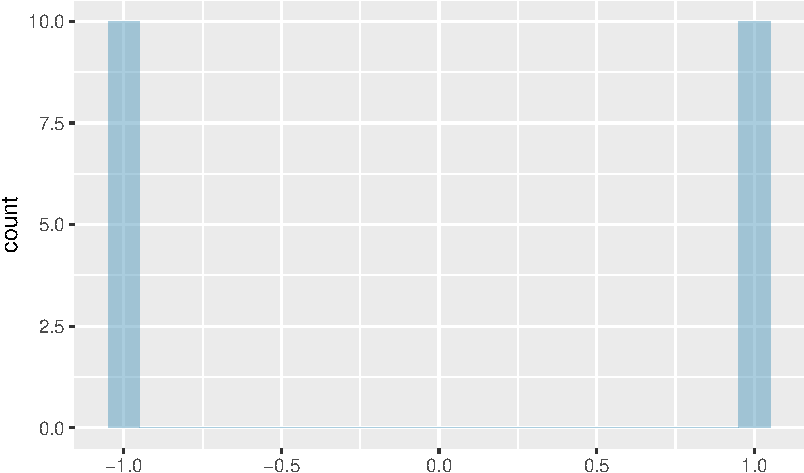
\includegraphics{05-Numerical-Data_files/figure-latex/hist53-fig-1.pdf}
\caption{\label{fig:hist53-fig}The first of three very different population distributions with the same mean, 0, and standard deviation, 1.}
\end{figure}

\begin{figure}
\centering
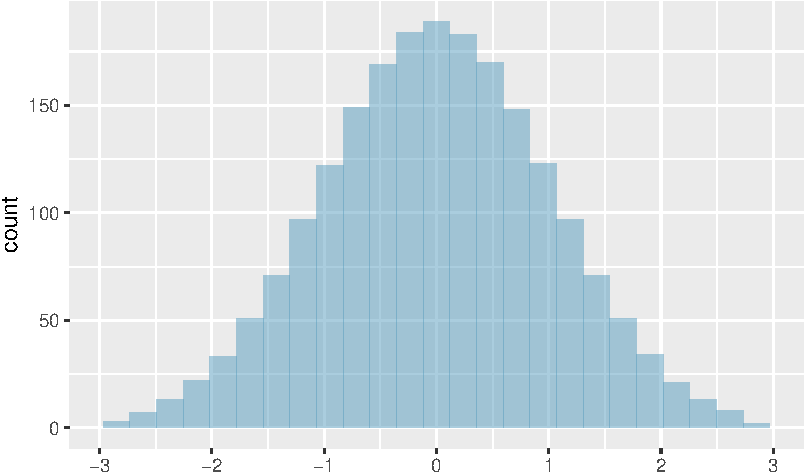
\includegraphics{05-Numerical-Data_files/figure-latex/hist54-fig-1.pdf}
\caption{\label{fig:hist54-fig}The second plot with mean 0 and standard deviation 1.}
\end{figure}

\begin{figure}
\centering
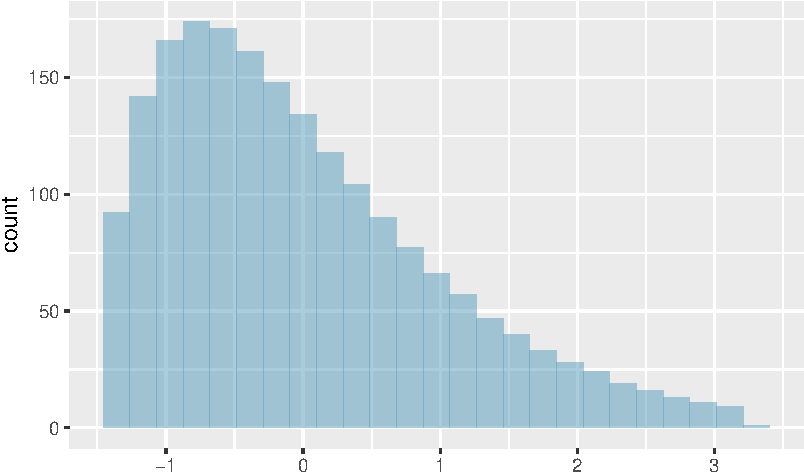
\includegraphics{05-Numerical-Data_files/figure-latex/hist55-fig-1.pdf}
\caption{\label{fig:hist55-fig}The final plot with mean 0 and standard deviation 1.}
\end{figure}

\begin{quote}
\textbf{Exercise}:\\
Earlier the concept of shape of a distribution was introduced. A good description of the shape of a distribution should include modality and whether the distribution is symmetric or skewed to one side. Using the three figures, Figures \ref{fig:hist53-fig}, \ref{fig:hist54-fig}, and \ref{fig:hist55-fig} as an example, explain why such a description is important.\footnote{Starting with Figure \ref{fig:hist53-fig}, the three figures show three distributions that look quite different, but all have the same mean, variance, and standard deviation. Using modality, we can distinguish between the first plot (bimodal) and the last two (unimodal). Using skewness, we can distinguish between the last plot (right skewed) and the first two. While a picture, like a histogram, tells a more complete story, we can use modality and shape (symmetry/skew) to characterize basic information about a distribution.}
\end{quote}

\begin{quote}
\emph{Example}:\\
Describe the distribution of the \texttt{num\_char} variable using the histogram in Figure \ref{fig:hist5-fig}. The description should incorporate the center, variability, and shape of the distribution, and it should also be placed in context: the number of characters in emails. Also note any especially unusual cases.\footnote{The distribution of email character counts is unimodal and very strongly skewed to the high end. Many of the counts fall near the mean at 11,600, and most fall within one standard deviation (13,130) of the mean. There is one exceptionally long email with about 65,000 characters.}
\end{quote}

In practice, the variance and standard deviation are sometimes used as a means to an end, where the \emph{end} is being able to accurately estimate the uncertainty associated with a sample statistic. For example, later in the course we will use the variance and standard deviation to assess how close the sample mean is to the population mean.

\hypertarget{box-plots-quartiles-and-the-median}{%
\subsection{Box plots, quartiles, and the median}\label{box-plots-quartiles-and-the-median}}

A \textbf{box plot} summarizes a data set using five statistics while also plotting unusual observations. Figure \ref{fig:box-fig} provides a vertical dot plot alongside a box plot of the \texttt{num\_char} variable from the \texttt{email50} data set.

\begin{figure}
\centering
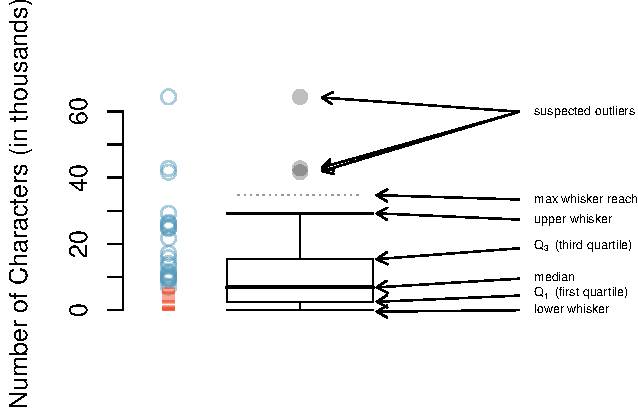
\includegraphics{05-Numerical-Data_files/figure-latex/box-fig-1.pdf}
\caption{\label{fig:box-fig}A vertical dot plot next to a labeled box plot for the number of characters in 50 emails. The median (6,890), splits the data into the bottom 50\% and the top 50\%, marked in the dot plot by horizontal dashes and open circles, respectively.}
\end{figure}

The first step in building a box plot is drawing a dark line denoting the \textbf{median}, which splits the data in half. Figure \ref{fig:box-fig} shows 50\% of the data falling below the median (red dashes) and the other 50\% falling above the median (blue open circles). There are 50 character counts in the data set (an even number) so the data are perfectly split into two groups of 25. We take the median in this case to be the average of the two observations closest to the \(50^{th}\) percentile: \((\text{6,768} + \text{7,012}) / 2 = \text{6,890}\). When there are an odd number of observations, there will be exactly one observation that splits the data into two halves, and in this case that observation is the median (no average needed).

\begin{quote}
\textbf{Median: the number in the middle}\\
If the data are ordered from smallest to largest, the \textbf{median} is the observation right in the middle. If there are an even number of observations, there will be two values in the middle, and the median is taken as their average.
\end{quote}

The second step in building a box plot is drawing a rectangle to represent the middle 50\% of the data. The total length of the box, shown vertically in Figure \ref{fig:box-fig}, is called the \textbf{interquartile range} (IQR, for short). It, like the standard deviation, is a measure of variability in data. The more variable the data, the larger the standard deviation and IQR. The two boundaries of the box are called the \textbf{first quartile} (the \(25^{th}\) percentile, i.e.~25\% of the data fall below this value) and the \textbf{third quartile} (the \(75^{th}\) percentile), and these are often labeled \(Q_1\) and \(Q_3\), respectively.

\begin{quote}
\textbf{Interquartile range (IQR)}\\
The IQR is the length of the box in a box plot. It is computed as
\[ IQR = Q_3 - Q_1 \]
where \(Q_1\) and \(Q_3\) are the \(25^{th}\) and \(75^{th}\) percentiles.
\end{quote}

\begin{quote}
\textbf{Exercise}:\\
What percent of the data fall between \(Q_1\) and the median? What percent is between the median and \(Q_3\)?\footnote{Since \(Q_1\) and \(Q_3\) capture the middle 50\% of the data and the median splits the data in the middle, 25\% of the data fall between \(Q_1\) and the median, and another 25\% falls between the median and \(Q_3\).}
\end{quote}

Extending out from the box, the \textbf{whiskers} attempt to capture the data outside of the box, however, their reach is never allowed to be more than \(1.5\times IQR\).\footnote{While the choice of exactly 1.5 is arbitrary, it is the most commonly used value for box plots.} They capture everything within this reach. In Figure \ref{fig:box-fig}, the upper whisker does not extend to the last three points, which are beyond \(Q_3 + 1.5\times IQR\), and so it extends only to the last point below this limit. The lower whisker stops at the lowest value, 33, since there is no additional data to reach; the lower whisker's limit is not shown in the figure because the plot does not extend down to \(Q_1 - 1.5\times IQR\). In a sense, the box is like the body of the box plot and the whiskers are like its arms trying to reach the rest of the data.

Any observation that lies beyond the whiskers is labeled with a dot. The purpose of labeling these points -- instead of just extending the whiskers to the minimum and maximum observed values -- is to help identify any observations that appear to be unusually distant from the rest of the data. Unusually distant observations are called \textbf{outliers}. In this case, it would be reasonable to classify the emails with character counts of 41,623, 42,793, and 64,401 as outliers since they are numerically distant from most of the data.

\begin{quote}
\textbf{Outliers are extreme}\\
An \textbf{outlier} is an observation that is extreme relative to the rest of the data.
\end{quote}

\begin{quote}
\textbf{Why it is important to look for outliers}\\
Examination of data for possible outliers serves many useful purposes, including\\
1. Identifying \textbf{strong skew} in the distribution.\\
2. Identifying data collection or entry errors. For instance, we re-examined the email purported to have 64,401 characters to ensure this value was accurate.\\
3. Providing insight into interesting properties of the data.
\end{quote}

\begin{quote}
\textbf{Exercise}:\\
The observation with value 64,401, an outlier, was found to be an accurate observation. What would such an observation suggest about the nature of character counts in emails?\footnote{That occasionally there may be very long emails.}
\end{quote}

\begin{quote}
\textbf{Exercise}:\\
Using Figure \ref{fig:box-fig}, estimate the following values for \texttt{num\_char} in the \texttt{email50} data set:\\
(a) \(Q_1\),\\
(b) \(Q_3\), and\\
(c) IQR.\footnote{These visual estimates will vary a little from one person to the next: \(Q_1\) \textasciitilde{} 3,000, \(Q_3\) \textasciitilde{} 15,000, IQR=\(Q_3 - Q_1\) \textasciitilde{} 12,000. (The true values: \(Q_1=\) 2,536, \(Q_3=\) 15,411, IQR = 12,875.)}
\end{quote}

Of course \texttt{R} can calculate these summary statistics for us. First we will do these calculations individually and then in one function call. Remember to ask what you want \texttt{R} to do and what it needs.

\begin{Shaded}
\begin{Highlighting}[]
\FunctionTok{mean}\NormalTok{(}\SpecialCharTok{\textasciitilde{}}\NormalTok{num\_char,}\AttributeTok{data=}\NormalTok{email50)}
\end{Highlighting}
\end{Shaded}

\begin{verbatim}
## [1] 11.59822
\end{verbatim}

\begin{Shaded}
\begin{Highlighting}[]
\FunctionTok{sd}\NormalTok{(}\SpecialCharTok{\textasciitilde{}}\NormalTok{num\_char,}\AttributeTok{data=}\NormalTok{email50)}
\end{Highlighting}
\end{Shaded}

\begin{verbatim}
## [1] 13.12526
\end{verbatim}

\begin{Shaded}
\begin{Highlighting}[]
\FunctionTok{quantile}\NormalTok{(}\SpecialCharTok{\textasciitilde{}}\NormalTok{num\_char,}\AttributeTok{data=}\NormalTok{email50)}
\end{Highlighting}
\end{Shaded}

\begin{verbatim}
##       0%      25%      50%      75%     100% 
##  0.05700  2.53550  6.88950 15.41075 64.40100
\end{verbatim}

\begin{Shaded}
\begin{Highlighting}[]
\FunctionTok{iqr}\NormalTok{(}\SpecialCharTok{\textasciitilde{}}\NormalTok{num\_char,}\AttributeTok{data=}\NormalTok{email50)}
\end{Highlighting}
\end{Shaded}

\begin{verbatim}
## [1] 12.87525
\end{verbatim}

\begin{Shaded}
\begin{Highlighting}[]
\FunctionTok{favstats}\NormalTok{(}\SpecialCharTok{\textasciitilde{}}\NormalTok{num\_char,}\AttributeTok{data=}\NormalTok{email50)}
\end{Highlighting}
\end{Shaded}

\begin{verbatim}
##    min     Q1 median       Q3    max     mean       sd  n missing
##  0.057 2.5355 6.8895 15.41075 64.401 11.59822 13.12526 50       0
\end{verbatim}

\hypertarget{robust-statistics}{%
\subsection{Robust statistics}\label{robust-statistics}}

How are the \emph{sample statistics} of the \texttt{num\_char} data set affected by the observation with value 64,401? What would have happened if this email wasn't observed? What would happen to these \emph{summary statistics} if the observation at 64,401 had been even larger, say 150,000? These scenarios are plotted alongside the original data in Figure \ref{fig:box2-fig}, and sample statistics are computed in \texttt{R}.

\begin{figure}
\centering
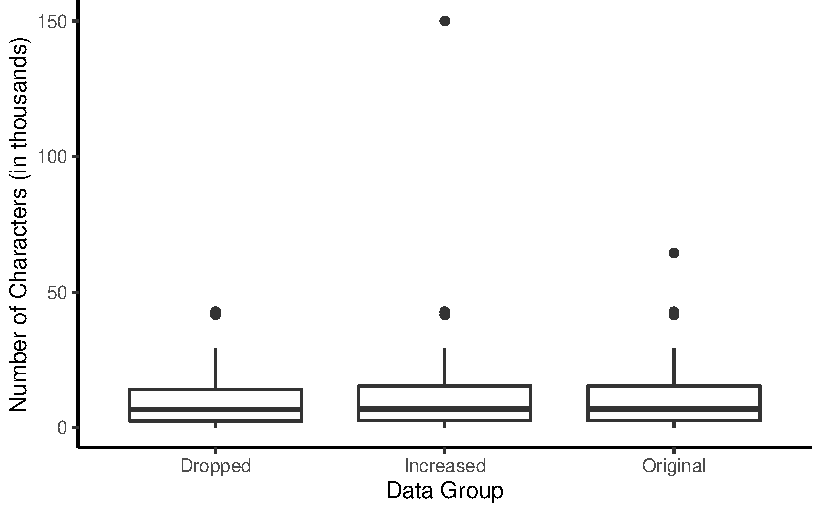
\includegraphics{05-Numerical-Data_files/figure-latex/box2-fig-1.pdf}
\caption{\label{fig:box2-fig}Box plots of the original character count data and two modified data sets.}
\end{figure}

\begin{verbatim}
##       group   min     Q1 median       Q3     max     mean       sd  n missing
## 1   Dropped 0.057 2.4540 6.7680 14.15600  42.793 10.52061 10.79768 49       0
## 2 Increased 0.057 2.5355 6.8895 15.41075 150.000 13.31020 22.43436 50       0
## 3  Original 0.057 2.5355 6.8895 15.41075  64.401 11.59822 13.12526 50       0
\end{verbatim}

The code used to generate this table is

\begin{Shaded}
\begin{Highlighting}[]
\NormalTok{p1 }\OtherTok{\textless{}{-}}\NormalTok{ email50}\SpecialCharTok{$}\NormalTok{num\_char}
\NormalTok{p2 }\OtherTok{\textless{}{-}}\NormalTok{ p1[}\SpecialCharTok{{-}}\FunctionTok{which.max}\NormalTok{(p1)]}
\NormalTok{p3 }\OtherTok{\textless{}{-}}\NormalTok{ p1}
\NormalTok{p3[}\FunctionTok{which.max}\NormalTok{(p1)] }\OtherTok{\textless{}{-}} \DecValTok{150}

\NormalTok{robust }\OtherTok{\textless{}{-}} \FunctionTok{data.frame}\NormalTok{(}\AttributeTok{value=} \FunctionTok{c}\NormalTok{(p1,p2,p3),}\AttributeTok{group=}\FunctionTok{c}\NormalTok{(}\FunctionTok{rep}\NormalTok{(}\StringTok{"Original"}\NormalTok{,}\DecValTok{50}\NormalTok{),}\FunctionTok{rep}\NormalTok{(}\StringTok{"Dropped"}\NormalTok{,}\DecValTok{49}\NormalTok{),}\FunctionTok{rep}\NormalTok{(}\StringTok{"Increased"}\NormalTok{,}\DecValTok{50}\NormalTok{)))}

\FunctionTok{favstats}\NormalTok{(value}\SpecialCharTok{\textasciitilde{}}\NormalTok{group,}\AttributeTok{data=}\NormalTok{robust)}
\end{Highlighting}
\end{Shaded}

Notice by using the formula notation, we were able to calculate the summary statistics for each group.

\begin{quote}
\textbf{Exercise}:\\
(a) Which is more affected by extreme observations, the mean or median? The data summary may be helpful.\\
(b) Is the standard deviation or IQR more affected by extreme observations?\footnote{(a) Mean is affected more. (b) Standard deviation is affected more.}
\end{quote}

The median and IQR are called \textbf{robust estimates} because extreme observations have little effect on their values. The mean and standard deviation are much more affected by changes in extreme observations.

\begin{quote}
\emph{Example}:\\
The median and IQR do not change much under the three scenarios above. Why might this be the case?\footnote{The median and IQR are only sensitive to numbers near \(Q_1\), the median, and \(Q_3\). Since values in these regions are relatively stable -- there aren't large jumps between observations -- the median and IQR estimates are also quite stable.}
\end{quote}

\begin{quote}
\textbf{Exercise}:\\
The distribution of vehicle prices tends to be right skewed, with a few luxury and sports cars lingering out into the right tail. If you were searching for a new car and cared about price, should you be more interested in the mean or median price of vehicles sold, assuming you are in the market for a regular car?\footnote{Buyers of a \emph{regular car} should be concerned about the median price. High-end car sales can drastically inflate the mean price while the median will be more robust to the influence of those sales.}
\end{quote}

\hypertarget{transforming-data}{%
\subsection{Transforming data}\label{transforming-data}}

When data are very strongly skewed, we sometimes transform them so they are easier to model. Consider the histogram of salaries for Major League Baseball players' salaries from 2010, which is shown in Figure \ref{fig:hist510-fig}.

\begin{figure}
\centering
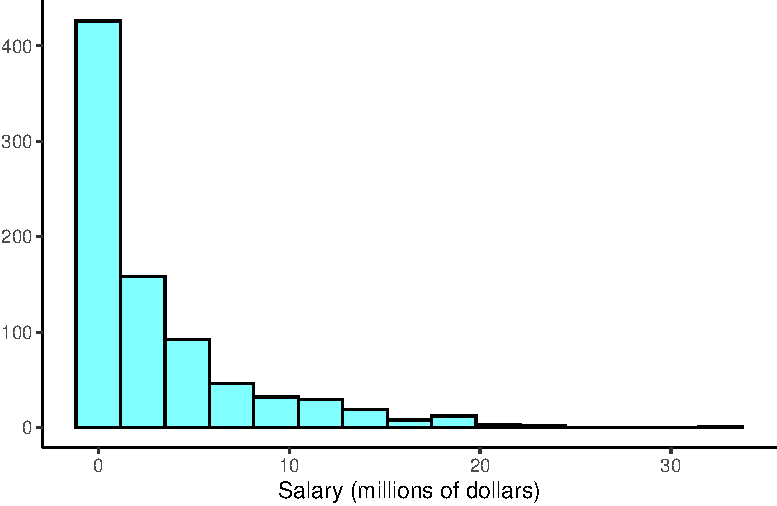
\includegraphics{05-Numerical-Data_files/figure-latex/hist510-fig-1.pdf}
\caption{\label{fig:hist510-fig}Histogram of MLB player salaries for 2010, in millions of dollars.}
\end{figure}

\begin{quote}
\emph{Example}:\\
The histogram of MLB player salaries is useful in that we can see the data are extremely skewed and centered (as gauged by the median) at about \$1 million. What isn't useful about this plot?\footnote{Most of the data are collected into one bin in the histogram and the data are so strongly skewed that many details in the data are obscured.}
\end{quote}

There are some standard transformations that are often applied when much of the data cluster near zero (relative to the larger values in the data set) and all observations are positive. A \textbf{transformation} is a rescaling of the data using a function. For instance, a plot of the natural logarithm\footnote{Statisticians often write the natural logarithm as \(\log\). You might be more familiar with it being written as \(\ln\).} of player salaries results in a new histogram in Figure \ref{fig:hist512-fig}. Transformed data are sometimes easier to work with when applying statistical models because the transformed data are much less skewed and outliers are usually less extreme.

\begin{figure}
\centering
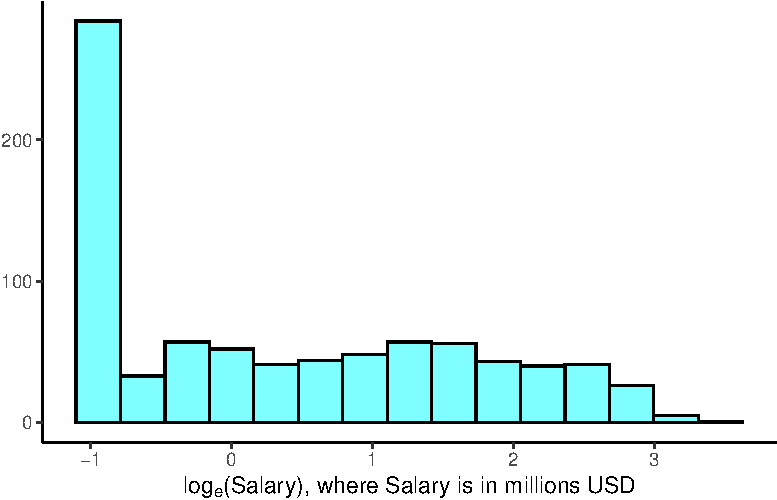
\includegraphics{05-Numerical-Data_files/figure-latex/hist512-fig-1.pdf}
\caption{\label{fig:hist512-fig}Histogram of the log-transformed MLB player salaries for 2010.}
\end{figure}

Transformations can also be applied to one or both variables in a scatterplot. A scatterplot of the \texttt{line\_breaks} and \texttt{num\_char} variables is shown in Figure \ref{fig:scat52-fig} above. We can see a positive association between the variables and that many observations are clustered near zero. Later in this course, we might want to use a straight line to model the data. However, we'll find that the data in their current state cannot be modeled very well. Figure \ref{fig:scat513-fig} shows a scatterplot where both the \texttt{line\_breaks} and \texttt{num\_char} variables have been transformed using a log (base \(e\)) transformation. While there is a positive association in each plot, the transformed data show a steadier trend, which is easier to model than the untransformed data.

\begin{figure}
\centering
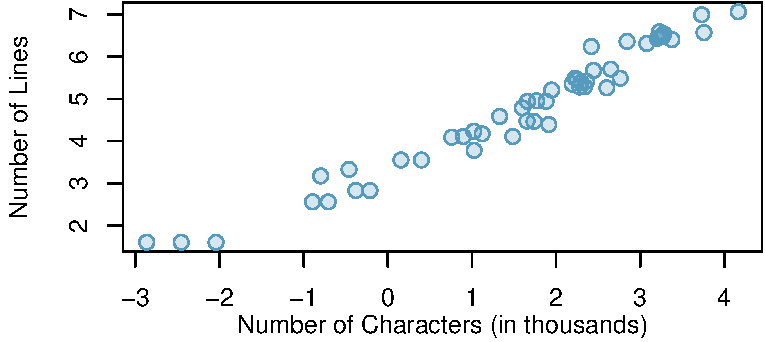
\includegraphics{05-Numerical-Data_files/figure-latex/scat513-fig-1.pdf}
\caption{\label{fig:scat513-fig}A scatterplot of \texttt{line\_breaks} versus \texttt{num\_char} for the \texttt{email50} data but where each variable has been log-transformed.}
\end{figure}

Transformations other than the logarithm can be useful, too. For instance, the square root (\(\sqrt{\text{original observation}}\)) and inverse (\(\frac{1}{\text{original observation}}\)) are used by statisticians. Common goals in transforming data are to see the data structure differently, reduce skew, assist in modeling, or straighten a nonlinear relationship in a scatterplot.

\hypertarget{homework-problems-4}{%
\section{Homework Problems}\label{homework-problems-4}}

Create an Rmd file for the work including headers, file creation data, and explanation of your work. Make sure your plots have a title and the axes are labeled. We are asking you to do more in this application to get ready for your Oral Board.

\begin{enumerate}
\def\labelenumi{\arabic{enumi}.}
\tightlist
\item
  \textbf{Mammals exploratory}
\end{enumerate}

Data were collected on 39 species of mammals distributed over 13 orders. The data is in the \textbf{openintro} package as \texttt{mammals}

\begin{enumerate}
\def\labelenumi{\alph{enumi}.}
\tightlist
\item
  Using help, report the units for the variable \texttt{brain\_Wt}.\\
\item
  Using \texttt{inspect} how many variables are numeric?\\
\item
  What type of variable is \texttt{danger}?
\item
  Create a histogram of \texttt{total\_sleep} and describe the distribution.\\
\item
  Create a boxplot of \texttt{life\_span} and describe the distribution.\\
\item
  Report the mean and median life span of a mammal.\\
\item
  Calculate the summary statistics for \texttt{life\_span} broken down by \texttt{danger}. What is the standard deviation of life span in danger outcome 5?
\end{enumerate}

\begin{enumerate}
\def\labelenumi{\arabic{enumi}.}
\setcounter{enumi}{1}
\tightlist
\item
  \textbf{Mammals life spans}
\end{enumerate}

Continue using the \texttt{mammals} data set.

\begin{enumerate}
\def\labelenumi{\alph{enumi}.}
\tightlist
\item
  Create side-by-side boxplots for \texttt{life\_span} broken down by \texttt{exposure}. Note: you will have to change \texttt{exposure} to a \texttt{factor()}. Report on any findings.\\
\item
  What happened to the median and third quartile in exposure group 4?
\item
  Create faceted histograms. What are the shortcomings of this plot?
\item
  Create a new variable \texttt{exposed} that is a factor with level \texttt{Low} if exposure is \texttt{1} or \texttt{2} and \texttt{High} otherwise.
\item
  Repeat part c with the new variable. Explain what you see in the plot.
\end{enumerate}

\begin{enumerate}
\def\labelenumi{\arabic{enumi}.}
\setcounter{enumi}{2}
\tightlist
\item
  \textbf{Mammals life spans continued}
\end{enumerate}

\begin{enumerate}
\def\labelenumi{\alph{enumi}.}
\tightlist
\item
  Create a scatterplot of life span versus length of gestation.\\
\item
  What type of an association is apparent between life span and length of gestation?\\
\item
  What type of an association would you expect to see if the axes of the plot were reversed, i.e.~if we plotted length of gestation versus life span?
\item
  Create the new scatterplot suggested in c.\\
\item
  Are life span and length of gestation independent? Explain your reasoning.
\end{enumerate}

\hypertarget{CATDATA}{%
\chapter{Categorical Data}\label{CATDATA}}

\hypertarget{objectives-5}{%
\section{Objectives}\label{objectives-5}}

\begin{enumerate}
\def\labelenumi{\arabic{enumi})}
\tightlist
\item
  Define and use properly in context all new terminology.
\item
  Generate in \texttt{R} tables for categorical variable(s).\\
\item
  Generate in \texttt{R} appropriate graphical summaries of categorical and numerical variables.\\
\item
  Be able to interpret and explain output both graphically and numerically.
\end{enumerate}

\hypertarget{categorical-data}{%
\section{Categorical data}\label{categorical-data}}

Like numerical data, categorical data can also be organized and analyzed. This section introduces tables and other basic tools for categorical data. Remember at the beginning of this block of material, our case study had categorical data so we have seen some of the ideas in this lesson.

The \texttt{email50} data set represents a sample from a larger email data set called \texttt{email}. This larger data set contains information on 3,921 emails. In this section we will use the email data set to examine whether the presence of numbers, small or large, in an email provides any useful value in classifying email as spam or not spam.

\hypertarget{contingency-tables-and-bar-plots}{%
\subsection{Contingency tables and bar plots}\label{contingency-tables-and-bar-plots}}

In the \texttt{email} data set we have two variables: \texttt{spam} and \texttt{number} that we want to summarize. Let's use \texttt{inspect()} to get information and insight about the two variables. We can also type \texttt{?email} to learn more about the data. First load the \texttt{openintro} library.

\begin{Shaded}
\begin{Highlighting}[]
\FunctionTok{library}\NormalTok{(openintro)}
\end{Highlighting}
\end{Shaded}

\begin{Shaded}
\begin{Highlighting}[]
\NormalTok{email }\SpecialCharTok{\%\textgreater{}\%}
  \FunctionTok{select}\NormalTok{(spam,number) }\SpecialCharTok{\%\textgreater{}\%}
  \FunctionTok{inspect}\NormalTok{()}
\end{Highlighting}
\end{Shaded}

\begin{verbatim}
## 
## categorical variables:  
##     name  class levels    n missing
## 1   spam factor      2 3921       0
## 2 number factor      3 3921       0
##                                    distribution
## 1 0 (90.6%), 1 (9.4%)                          
## 2 small (72.1%), none (14%) ...
\end{verbatim}

Notice the use of the \texttt{pipe} operator and how it adds to the ease of reading the code. The \texttt{select()} function allows us to narrow the variables down to the two of interest. Then \texttt{inspect()} gives us information about those variables. We read from top line; we start with the data set \texttt{email}, input it into \texttt{select()} and select variables from it, and then use \texttt{inspect()} to summarize the variables.

As is indicated \texttt{number} is a categorical variable that describes whether an email contains no numbers, only small numbers (values under 1 million), or at least one big number (a value of 1 million or more). The variable \texttt{spam} is a numeric variable where \texttt{1} indicates the email is spam. To treat it as categorical we will want to change it to a \textbf{factor} but first we will build a table that summarizes data for the two variables, see Table \ref{tab:contin1-tab}. This table is called a \textbf{contingency table}. Each value in the table represents the number of times a particular combination of variable outcomes occurred. We will show you the code to generate the contingency table.

\begin{table}

\caption{\label{tab:contin1-tab}A contingency table for the `email` data.}
\centering
\begin{tabular}[t]{lrrrr}
\toprule
\multicolumn{1}{c}{Spam} & \multicolumn{3}{c}{Number} & \multicolumn{1}{c}{ } \\
\cmidrule(l{3pt}r{3pt}){1-1} \cmidrule(l{3pt}r{3pt}){2-4}
  & none & small & big & Total\\
\midrule
0 & 400 & 2659 & 495 & 3554\\
1 & 149 & 168 & 50 & 367\\
Total & 549 & 2827 & 545 & 3921\\
\bottomrule
\end{tabular}
\end{table}

\begin{Shaded}
\begin{Highlighting}[]
\FunctionTok{tally}\NormalTok{(}\SpecialCharTok{\textasciitilde{}}\NormalTok{spam}\SpecialCharTok{+}\NormalTok{number,}\AttributeTok{data=}\NormalTok{email,}\AttributeTok{margins =} \ConstantTok{TRUE}\NormalTok{)}
\end{Highlighting}
\end{Shaded}

\begin{verbatim}
##        number
## spam    none small  big Total
##   0      400  2659  495  3554
##   1      149   168   50   367
##   Total  549  2827  545  3921
\end{verbatim}

The value 149 corresponds to the number of emails in the data set that are spam \emph{and} had no number listed in the email. Row and column totals are also included. The \textbf{row totals} provide the total counts across each row (e.g.~\(149 + 168 + 50 = 367\)), and \textbf{column totals} are total counts down each column. The row and column totals are known as \textbf{marginal} counts and the values in the table, such as 149, as \textbf{joint} counts.

Let's turn \texttt{spam} into a factor and update the \texttt{email} data object. We will use \texttt{mutate()} to do this.

\begin{Shaded}
\begin{Highlighting}[]
\NormalTok{email }\OtherTok{\textless{}{-}}\NormalTok{ email }\SpecialCharTok{\%\textgreater{}\%}
  \FunctionTok{mutate}\NormalTok{(}\AttributeTok{spam =} \FunctionTok{factor}\NormalTok{(email}\SpecialCharTok{$}\NormalTok{spam,}\AttributeTok{levels=}\FunctionTok{c}\NormalTok{(}\DecValTok{1}\NormalTok{,}\DecValTok{0}\NormalTok{),}\AttributeTok{labels=}\FunctionTok{c}\NormalTok{(}\StringTok{"spam"}\NormalTok{,}\StringTok{"not spam"}\NormalTok{)))}
\end{Highlighting}
\end{Shaded}

Now checking the data again.

\begin{Shaded}
\begin{Highlighting}[]
\NormalTok{email }\SpecialCharTok{\%\textgreater{}\%}
  \FunctionTok{select}\NormalTok{(spam,number) }\SpecialCharTok{\%\textgreater{}\%}
  \FunctionTok{inspect}\NormalTok{()}
\end{Highlighting}
\end{Shaded}

\begin{verbatim}
## 
## categorical variables:  
##     name  class levels    n missing
## 1   spam factor      2 3921       0
## 2 number factor      3 3921       0
##                                    distribution
## 1 not spam (90.6%), spam (9.4%)                
## 2 small (72.1%), none (14%) ...
\end{verbatim}

Let's generate the table again.

\begin{Shaded}
\begin{Highlighting}[]
\FunctionTok{tally}\NormalTok{(}\SpecialCharTok{\textasciitilde{}}\NormalTok{spam}\SpecialCharTok{+}\NormalTok{number,}\AttributeTok{data=}\NormalTok{email,}\AttributeTok{margins =} \ConstantTok{TRUE}\NormalTok{)}
\end{Highlighting}
\end{Shaded}

\begin{verbatim}
##           number
## spam       none small  big Total
##   spam      149   168   50   367
##   not spam  400  2659  495  3554
##   Total     549  2827  545  3921
\end{verbatim}

A table for a single variable is called a \textbf{frequency table}. The table below is a frequency table for the \texttt{number} variable.

\begin{Shaded}
\begin{Highlighting}[]
\FunctionTok{tally}\NormalTok{(}\SpecialCharTok{\textasciitilde{}}\NormalTok{number,}\AttributeTok{data=}\NormalTok{email)}
\end{Highlighting}
\end{Shaded}

\begin{verbatim}
## number
##  none small   big 
##   549  2827   545
\end{verbatim}

If we replaced the counts with percentages or proportions, the table would be called a \textbf{relative frequency table}.

\begin{Shaded}
\begin{Highlighting}[]
\FunctionTok{tally}\NormalTok{(}\SpecialCharTok{\textasciitilde{}}\NormalTok{number,}\AttributeTok{data=}\NormalTok{email,}\AttributeTok{format=}\StringTok{\textquotesingle{}proportion\textquotesingle{}}\NormalTok{)}
\end{Highlighting}
\end{Shaded}

\begin{verbatim}
## number
##      none     small       big 
## 0.1400153 0.7209895 0.1389952
\end{verbatim}

\begin{Shaded}
\begin{Highlighting}[]
\FunctionTok{round}\NormalTok{(}\FunctionTok{tally}\NormalTok{(}\SpecialCharTok{\textasciitilde{}}\NormalTok{number,}\AttributeTok{data=}\NormalTok{email,}\AttributeTok{format=}\StringTok{\textquotesingle{}percent\textquotesingle{}}\NormalTok{),}\DecValTok{2}\NormalTok{)}
\end{Highlighting}
\end{Shaded}

\begin{verbatim}
## number
##  none small   big 
##  14.0  72.1  13.9
\end{verbatim}

A bar plot is a common way to display a single categorical variable. Figure \ref{fig:bar61-fig} shows a \textbf{bar plot} for the \texttt{number} variable.



\begin{Shaded}
\begin{Highlighting}[]
\NormalTok{email }\SpecialCharTok{\%\textgreater{}\%}
  \FunctionTok{gf\_bar}\NormalTok{(}\SpecialCharTok{\textasciitilde{}}\NormalTok{number) }\SpecialCharTok{\%\textgreater{}\%}
  \FunctionTok{gf\_theme}\NormalTok{(}\FunctionTok{theme\_bw}\NormalTok{()) }\SpecialCharTok{\%\textgreater{}\%}
  \FunctionTok{gf\_labs}\NormalTok{(}\AttributeTok{x=}\StringTok{"Size of Number"}\NormalTok{,}\AttributeTok{y=}\StringTok{"Count"}\NormalTok{)}
\end{Highlighting}
\end{Shaded}

\begin{figure}
\centering
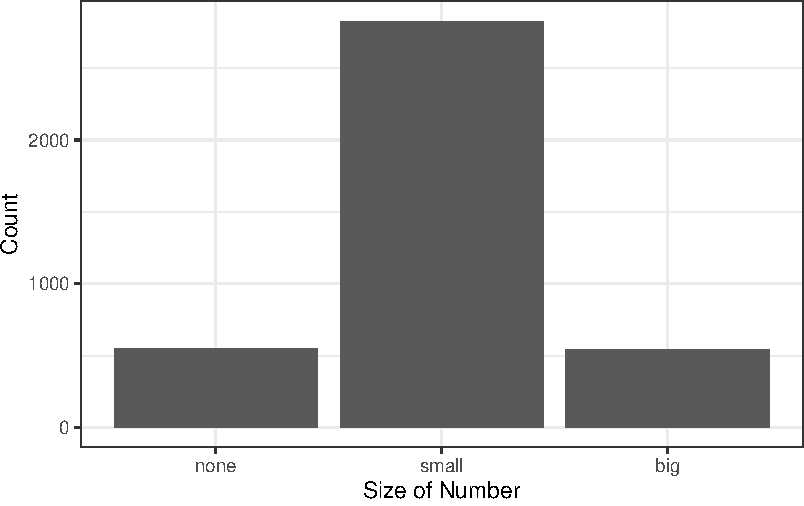
\includegraphics{06-Categorical-Data_files/figure-latex/bar61-fig-1.pdf}
\caption{\label{fig:bar61-fig}Bar chart of the \texttt{number} variable.}
\end{figure}

Next the counts are converted into proportions (e.g.~\(549/3921=0.140\) for \texttt{none}) in Figure \ref{fig:bar62-fig}.



\begin{Shaded}
\begin{Highlighting}[]
\NormalTok{email }\SpecialCharTok{\%\textgreater{}\%}
  \FunctionTok{gf\_props}\NormalTok{(}\SpecialCharTok{\textasciitilde{}}\NormalTok{number) }\SpecialCharTok{\%\textgreater{}\%}
  \FunctionTok{gf\_theme}\NormalTok{(}\FunctionTok{theme\_bw}\NormalTok{()) }\SpecialCharTok{\%\textgreater{}\%}
  \FunctionTok{gf\_labs}\NormalTok{(}\AttributeTok{x=}\StringTok{"Size of Number"}\NormalTok{,}\AttributeTok{y=}\StringTok{"Proportion"}\NormalTok{)}
\end{Highlighting}
\end{Shaded}

\begin{figure}
\centering
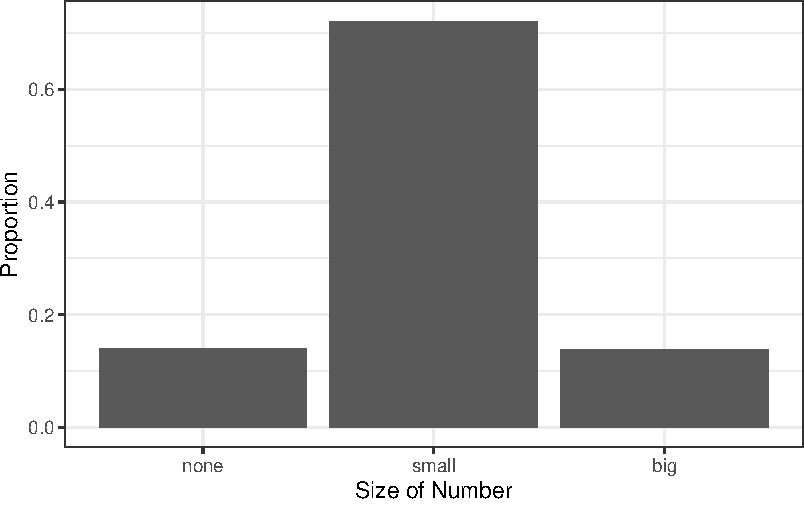
\includegraphics{06-Categorical-Data_files/figure-latex/bar62-fig-1.pdf}
\caption{\label{fig:bar62-fig}(ref:quote62}
\end{figure}

Again, let's clean up the plot into a style that we could use in a report.

\begin{Shaded}
\begin{Highlighting}[]
\NormalTok{email }\SpecialCharTok{\%\textgreater{}\%}
  \FunctionTok{gf\_props}\NormalTok{(}\SpecialCharTok{\textasciitilde{}}\NormalTok{number,}\AttributeTok{title=}\StringTok{"The proportions of emails with a number in it"}\NormalTok{,}
           \AttributeTok{subtitle=}\StringTok{"From 2012"}\NormalTok{,}\AttributeTok{xlab=}\StringTok{"Type of number in the email"}\NormalTok{,}
           \AttributeTok{ylab=}\StringTok{"Proportion of emails"}\NormalTok{) }\SpecialCharTok{\%\textgreater{}\%}
  \FunctionTok{gf\_theme}\NormalTok{(}\FunctionTok{theme\_bw}\NormalTok{())}
\end{Highlighting}
\end{Shaded}

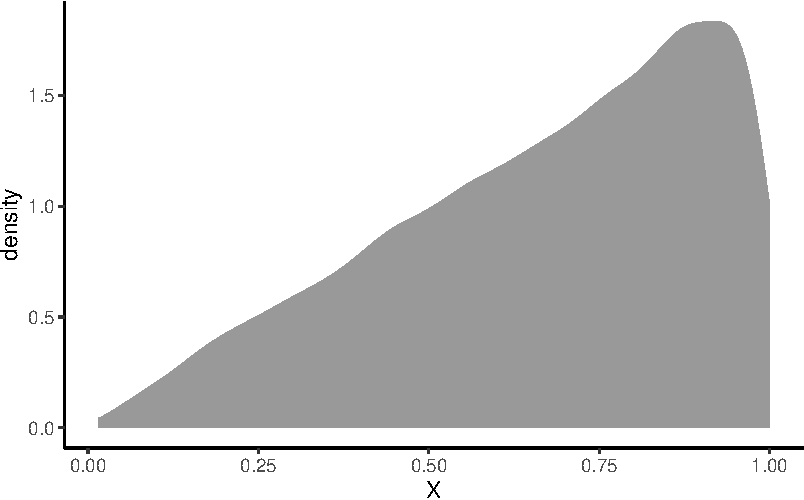
\includegraphics{06-Categorical-Data_files/figure-latex/unnamed-chunk-11-1.pdf}

\hypertarget{column-proportions}{%
\subsection{Column proportions}\label{column-proportions}}

The table below shows the column proportions. The \textbf{column proportions} are computed as the counts divided by their column totals. The value 149 at the intersection of \emph{spam} and \emph{none} is replaced by \(149/549=0.271\), i.e.~149 divided by its row total, 549. So what does 0.271 represent? It corresponds to the proportion of emails in the sample with no numbers that are spam. We are \textbf{conditioning}, restricting, on emails with no number. This rate of spam is much higher than emails with only small numbers (5.9\%) or big numbers (9.2\%). Because these spam rates vary between the three levels of \texttt{number} (\emph{none}, \emph{small}, \emph{big}), this provides evidence that the \texttt{spam} and \texttt{number} variables are associated.

\begin{Shaded}
\begin{Highlighting}[]
\FunctionTok{tally}\NormalTok{(spam}\SpecialCharTok{\textasciitilde{}}\NormalTok{number,}\AttributeTok{data=}\NormalTok{email,}\AttributeTok{margins =} \ConstantTok{TRUE}\NormalTok{,}\AttributeTok{format=}\StringTok{\textquotesingle{}proportion\textquotesingle{}}\NormalTok{)}
\end{Highlighting}
\end{Shaded}

\begin{verbatim}
##           number
## spam             none      small        big
##   spam     0.27140255 0.05942695 0.09174312
##   not spam 0.72859745 0.94057305 0.90825688
##   Total    1.00000000 1.00000000 1.00000000
\end{verbatim}

The \texttt{tally()} function will always condition on the variable on the right hand side of the tilde, \textasciitilde, when calculating proportions and thus only generate column proportions. The more general \texttt{table()} function of \texttt{R} will allow either column or row proportions.

\begin{quote}
\textbf{Exercise}:\\
Create a table of column proportions where the variable \texttt{spam} is the column variable.
\end{quote}

\begin{Shaded}
\begin{Highlighting}[]
\FunctionTok{tally}\NormalTok{(number}\SpecialCharTok{\textasciitilde{}}\NormalTok{spam,}\AttributeTok{data=}\NormalTok{email,}\AttributeTok{margins =} \ConstantTok{TRUE}\NormalTok{,}\AttributeTok{format=}\StringTok{\textquotesingle{}proportion\textquotesingle{}}\NormalTok{)}
\end{Highlighting}
\end{Shaded}

\begin{verbatim}
##        spam
## number       spam  not spam
##   none  0.4059946 0.1125492
##   small 0.4577657 0.7481711
##   big   0.1362398 0.1392797
##   Total 1.0000000 1.0000000
\end{verbatim}

\begin{quote}
\textbf{Exercise}:\\
In the table you just created, what does 0.748 represent?\footnote{0.748 represents the proportions of emails with no spam that had a small number in it.}
\end{quote}

\begin{quote}
\emph{Example}:\\
Data scientists use statistics to filter spam from incoming email messages. By noting specific characteristics of an email, a data scientist may be able to classify some emails as spam or not spam with high accuracy. One of those characteristics is whether the email contains no numbers, small numbers, or big numbers. Another characteristic is whether or not an email has any HTML content. A contingency table for the \texttt{spam} and \texttt{format} variables is needed.\\
1 Make \texttt{format} into a categorical factor variable.The levels should be ``text'' and ``HTML''.\footnote{From the help menu on the data HTML is coded as a 1}\\
2 Create a contingency table from the \texttt{email} data set with \texttt{format} in the columns and \texttt{spam} in the rows.
\end{quote}

In deciding which variable to use as a column, the data scientist would be interested in how the proportion of spam changes within each email format. This corresponds to column proportions based on \texttt{format}: the proportion of spam in plain text emails and the proportion of spam in HTML emails.

\begin{Shaded}
\begin{Highlighting}[]
\NormalTok{email }\OtherTok{\textless{}{-}}\NormalTok{ email }\SpecialCharTok{\%\textgreater{}\%}
  \FunctionTok{mutate}\NormalTok{(}\AttributeTok{format =} \FunctionTok{factor}\NormalTok{(email}\SpecialCharTok{$}\NormalTok{format,}\AttributeTok{levels=}\FunctionTok{c}\NormalTok{(}\DecValTok{1}\NormalTok{,}\DecValTok{0}\NormalTok{),}\AttributeTok{labels=}\FunctionTok{c}\NormalTok{(}\StringTok{"HTML"}\NormalTok{,}\StringTok{"text"}\NormalTok{)))}
\end{Highlighting}
\end{Shaded}

\begin{Shaded}
\begin{Highlighting}[]
\FunctionTok{tally}\NormalTok{(spam}\SpecialCharTok{\textasciitilde{}}\NormalTok{format,}\AttributeTok{data=}\NormalTok{email,}\AttributeTok{margins =} \ConstantTok{TRUE}\NormalTok{,}\AttributeTok{format=}\StringTok{"proportion"}\NormalTok{)}
\end{Highlighting}
\end{Shaded}

\begin{verbatim}
##           format
## spam             HTML       text
##   spam     0.05796038 0.17489540
##   not spam 0.94203962 0.82510460
##   Total    1.00000000 1.00000000
\end{verbatim}

In generating the column proportions, we can see that a higher fraction of plain text emails are spam (\(209/1195 = 17.5\%\)) than compared to HTML emails (\(158/2726 = 5.8\%\)). This information on its own is insufficient to classify an email as spam or not spam, as over 80\% of plain text emails are not spam. Yet, when we carefully combine this information with many other characteristics, such as \texttt{number} and other variables, we stand a reasonable chance of being able to classify some email as spam or not spam.

In constructing a table, we need to think about which variable we want in the column and which in the row. The formula format in some way makes us think about the response and predictor variables. However in some cases, it is not clear which variable should be in the column and row and the analyst must decide the point to be made with the table. Before settling on one form for a table, it is important to consider the audience and the message they are to receive from the table.

\begin{quote}
\textbf{Exercise}:\\
Create two tables with \texttt{number} and \texttt{spam} where each are in the column, so two table where you change which variable is in the column. Which would be more useful to someone hoping to identify spam emails using the \texttt{number} variable?\footnote{The column proportions with \texttt{number} in the columns will probably be most useful, which makes it easier to see that emails with small numbers are spam about 5.9\% of the time (relatively rare). We would also see that about 27.1\% of emails with no numbers are spam, and 9.2\% of emails with big numbers are spam.}
\end{quote}

\begin{Shaded}
\begin{Highlighting}[]
\FunctionTok{tally}\NormalTok{(spam}\SpecialCharTok{\textasciitilde{}}\NormalTok{number,email,}\AttributeTok{format=}\StringTok{\textquotesingle{}proportion\textquotesingle{}}\NormalTok{,}\AttributeTok{margin=}\ConstantTok{TRUE}\NormalTok{)}
\end{Highlighting}
\end{Shaded}

\begin{verbatim}
##           number
## spam             none      small        big
##   spam     0.27140255 0.05942695 0.09174312
##   not spam 0.72859745 0.94057305 0.90825688
##   Total    1.00000000 1.00000000 1.00000000
\end{verbatim}

\begin{Shaded}
\begin{Highlighting}[]
\FunctionTok{tally}\NormalTok{(number}\SpecialCharTok{\textasciitilde{}}\NormalTok{spam,email,}\AttributeTok{format=}\StringTok{\textquotesingle{}proportion\textquotesingle{}}\NormalTok{,}\AttributeTok{margin=}\ConstantTok{TRUE}\NormalTok{)}
\end{Highlighting}
\end{Shaded}

\begin{verbatim}
##        spam
## number       spam  not spam
##   none  0.4059946 0.1125492
##   small 0.4577657 0.7481711
##   big   0.1362398 0.1392797
##   Total 1.0000000 1.0000000
\end{verbatim}

\hypertarget{segmented-bar-and-mosaic-plots}{%
\subsection{Segmented bar and mosaic plots}\label{segmented-bar-and-mosaic-plots}}

Contingency tables using column proportions are especially useful for examining how two categorical variables are related. Segmented bar and mosaic plots provide a way to visualize the information in these tables.

A \textbf{segmented bar plot} is a graphical display of contingency table information. For example, a segmented bar plot representing the table with \texttt{number} in the column is shown in Figure \ref{fig:barseg61-fig}, where we have first created a bar plot using the \texttt{number} variable and then separated each group by the levels of \texttt{spam}.



\begin{Shaded}
\begin{Highlighting}[]
\NormalTok{email }\SpecialCharTok{\%\textgreater{}\%}
  \FunctionTok{gf\_bar}\NormalTok{(}\SpecialCharTok{\textasciitilde{}}\NormalTok{number,}\AttributeTok{fill=}\SpecialCharTok{\textasciitilde{}}\NormalTok{spam) }\SpecialCharTok{\%\textgreater{}\%}
  \FunctionTok{gf\_theme}\NormalTok{(}\FunctionTok{theme\_bw}\NormalTok{()) }\SpecialCharTok{\%\textgreater{}\%}
  \FunctionTok{gf\_labs}\NormalTok{(}\AttributeTok{x=}\StringTok{"Size of Number"}\NormalTok{,}\AttributeTok{y=}\StringTok{"Count"}\NormalTok{)}
\end{Highlighting}
\end{Shaded}

\begin{figure}
\centering
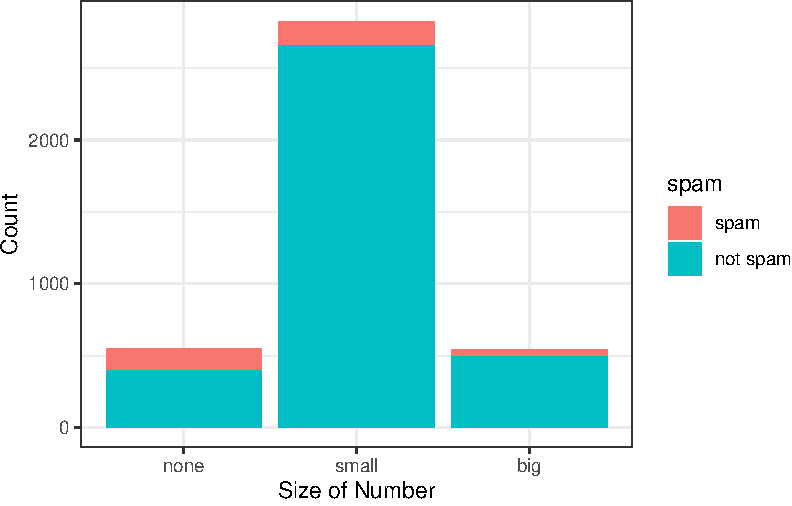
\includegraphics{06-Categorical-Data_files/figure-latex/barseg61-fig-1.pdf}
\caption{\label{fig:barseg61-fig}Segmented bar plot for numbers found in \texttt{emails}, where the counts have been further broken down by \texttt{spam}.}
\end{figure}

The column proportions of the table have been translated into a standardized segmented bar plot in Figure \ref{fig:barseg62-fig}, which is a helpful visualization of the fraction of spam emails in each level of \texttt{number}.



\begin{Shaded}
\begin{Highlighting}[]
\NormalTok{email }\SpecialCharTok{\%\textgreater{}\%}
  \FunctionTok{gf\_props}\NormalTok{(}\SpecialCharTok{\textasciitilde{}}\NormalTok{number,}\AttributeTok{fill=}\SpecialCharTok{\textasciitilde{}}\NormalTok{spam,}\AttributeTok{position=}\StringTok{\textquotesingle{}fill\textquotesingle{}}\NormalTok{) }\SpecialCharTok{\%\textgreater{}\%}
  \FunctionTok{gf\_theme}\NormalTok{(}\FunctionTok{theme\_bw}\NormalTok{()) }\SpecialCharTok{\%\textgreater{}\%}
  \FunctionTok{gf\_labs}\NormalTok{(}\AttributeTok{x=}\StringTok{"Size of Number"}\NormalTok{,}\AttributeTok{y=}\StringTok{"Proportion"}\NormalTok{)}
\end{Highlighting}
\end{Shaded}

\begin{figure}
\centering
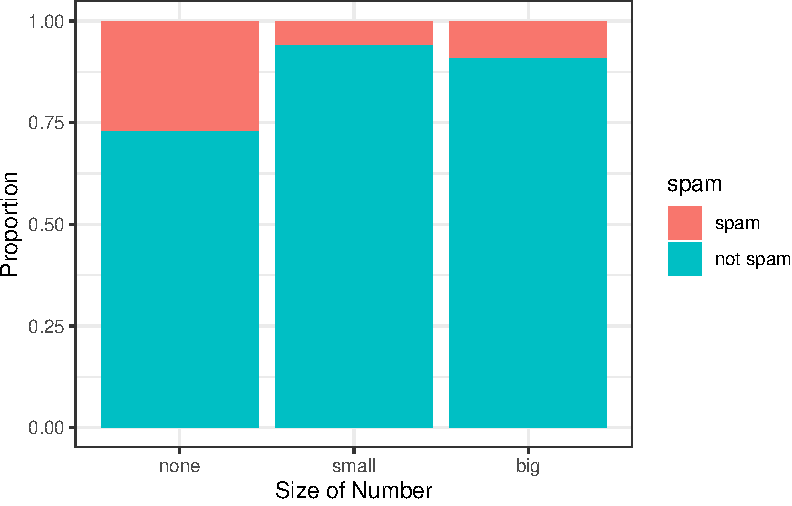
\includegraphics{06-Categorical-Data_files/figure-latex/barseg62-fig-1.pdf}
\caption{\label{fig:barseg62-fig}Standardized version of Figure \ref{fig:barseg61-fig}.}
\end{figure}

\begin{quote}
\emph{Example}:\\
Examine both of the segmented bar plots. Which is more useful?
\end{quote}

Figure \ref{fig:barseg61-fig} contains more information, but Figure \ref{fig:barseg62-fig} presents the information more clearly. This second plot makes it clear that emails with no number have a relatively high rate of spam email -- about 27\%! On the other hand, less than 10\% of email with small or big numbers are spam.

Since the proportion of spam changes across the groups in Figure \ref{fig:barseg62-fig}, we can conclude the variables are dependent, which is something we were also able to discern using table proportions. Because both the \texttt{none} and \texttt{big} groups have relatively few observations compared to the \texttt{small} group, the association is more difficult to see in Figure \ref{fig:barseg61-fig}.

In some other cases, a segmented bar plot that is not standardized will be more useful in communicating important information. Before settling on a particular segmented bar plot, create standardized and non-standardized forms and decide which is more effective at communicating features of the data.

A \textbf{mosaic plot} is a graphical display of contingency table information that is similar to a bar plot for one variable or a segmented bar plot when using two variables. It seems strange, but mosaic plots are not part of the \textbf{mosaic} package. We must load another set of packages called \textbf{vcd} and \textbf{vcdExtra}. Mosaic plot displays help to visualize the pattern of associations among variables in two-way and larger tables. Mosaic plots are controversial since they rely on the perception of area. Human vision is not good at distinguishing areas.

We will introduce mosaic plots because it is another way to visualize contingency tables. Figure \ref{fig:mosaic61-fig} shows a mosaic plot for the \texttt{number} variable. Each row represents a level of \texttt{number}, and the row heights correspond to the proportion of emails of each number type. For instance, there are fewer emails with no numbers than emails with only small numbers, so the \texttt{none} outcome row is shorter in height. In general, mosaic plots use box \emph{areas} to represent the number of observations. Since there is only one variable, the widths are all constant. Thus area is simply related to row height making this visual easy to read.

\begin{Shaded}
\begin{Highlighting}[]
\FunctionTok{library}\NormalTok{(vcd)}
\end{Highlighting}
\end{Shaded}



\begin{Shaded}
\begin{Highlighting}[]
\FunctionTok{mosaic}\NormalTok{(}\SpecialCharTok{\textasciitilde{}}\NormalTok{number,}\AttributeTok{data=}\NormalTok{email)}
\end{Highlighting}
\end{Shaded}

\begin{figure}
\centering
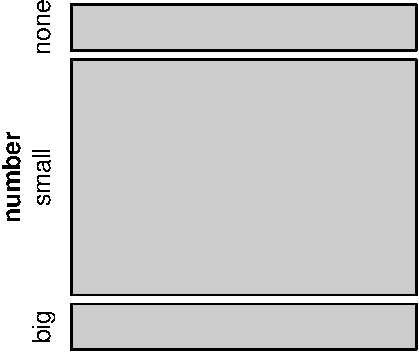
\includegraphics{06-Categorical-Data_files/figure-latex/mosaic61-fig-1.pdf}
\caption{\label{fig:mosaic61-fig}Mosaic plot where emails are grouped by the \texttt{number} variable.}
\end{figure}

This one-variable mosaic plot can be further divided into pieces as in Figure \ref{fig:mosaic62-fig} using the \texttt{spam} variable. The first variable in the formula is used to determine row height. That is, each row is split proportionally according to the fraction of emails in each number category, these heights are similar to Figure \ref{fig:mosaic61-fig}. Next each row is split horizontally according to the proportion of emails that were spam in that number group. For example, the second row, representing emails with only small numbers, was divided into emails that were spam (left) and not spam (right). The area of the rectangles is proportional to the proportions in the table where each cell count is divided by the total count. First we will generate the table and then represent it as a mosaic plot.

\begin{Shaded}
\begin{Highlighting}[]
\FunctionTok{tally}\NormalTok{(}\SpecialCharTok{\textasciitilde{}}\NormalTok{number}\SpecialCharTok{+}\NormalTok{spam,}\AttributeTok{data=}\NormalTok{email,}\AttributeTok{format=}\StringTok{\textquotesingle{}proportion\textquotesingle{}}\NormalTok{)}
\end{Highlighting}
\end{Shaded}

\begin{verbatim}
##        spam
## number        spam   not spam
##   none  0.03800051 0.10201479
##   small 0.04284621 0.67814333
##   big   0.01275185 0.12624331
\end{verbatim}



\begin{Shaded}
\begin{Highlighting}[]
\FunctionTok{mosaic}\NormalTok{(}\SpecialCharTok{\textasciitilde{}}\NormalTok{number}\SpecialCharTok{+}\NormalTok{spam,}\AttributeTok{data=}\NormalTok{email)}
\end{Highlighting}
\end{Shaded}

\begin{figure}
\centering
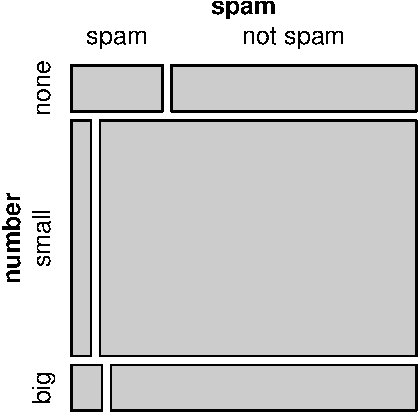
\includegraphics{06-Categorical-Data_files/figure-latex/mosaic62-fig-1.pdf}
\caption{\label{fig:mosaic62-fig}Mosaic plot with \texttt{number} as the first variable.}
\end{figure}

These plots are hard to use in a visual comparison of area. For example, is the area for \emph{small} number \emph{spam} emails different from \emph{none} number \emph{spam} emails? The rectangles have different shapes but from the table we can tell the areas are close.

An important use of the mosaic plot is to determine if an association between variables may be present. The bottom of the first column represents spam emails that had big numbers, and the bottom row of the second column represents regular emails that had big numbers. We can again use this plot to see that the \texttt{spam} and \texttt{number} variables are associated since some rows are divided in different vertical locations than others, which was the same technique used for checking an association in the standardized version of the segmented bar plot.

In a similar way, a mosaic plot representing column proportions where \emph{spam} is in the column could be constructed. To completely understand the mosaic plot as shown in Figure \ref{fig:mosaic63-fig} let's first find the proportions of \texttt{spam}.

\begin{Shaded}
\begin{Highlighting}[]
\FunctionTok{tally}\NormalTok{(}\SpecialCharTok{\textasciitilde{}}\NormalTok{spam,}\AttributeTok{data=}\NormalTok{email,}\AttributeTok{format=}\StringTok{"proportion"}\NormalTok{)}
\end{Highlighting}
\end{Shaded}

\begin{verbatim}
## spam
##       spam   not spam 
## 0.09359857 0.90640143
\end{verbatim}

So the row heights will be split 90-10. Next let's find the proportions of number within each value of spam. In the spam row, \emph{none} will be 41\%, \emph{small} will be 46\%, and \emph{big} will be 13\%.

\begin{Shaded}
\begin{Highlighting}[]
\FunctionTok{tally}\NormalTok{(number}\SpecialCharTok{\textasciitilde{}}\NormalTok{spam,}\AttributeTok{data=}\NormalTok{email,}\AttributeTok{margins =} \ConstantTok{TRUE}\NormalTok{,}\AttributeTok{format=}\StringTok{"proportion"}\NormalTok{)}
\end{Highlighting}
\end{Shaded}

\begin{verbatim}
##        spam
## number       spam  not spam
##   none  0.4059946 0.1125492
##   small 0.4577657 0.7481711
##   big   0.1362398 0.1392797
##   Total 1.0000000 1.0000000
\end{verbatim}

However, because it is more insightful for this application to consider the fraction of spam in each category of the \texttt{number} variable, we prefer Figure \ref{fig:mosaic62-fig}.



\begin{Shaded}
\begin{Highlighting}[]
\FunctionTok{mosaic}\NormalTok{(}\SpecialCharTok{\textasciitilde{}}\NormalTok{spam}\SpecialCharTok{+}\NormalTok{number,}\AttributeTok{data=}\NormalTok{email)}
\end{Highlighting}
\end{Shaded}

\begin{figure}
\centering
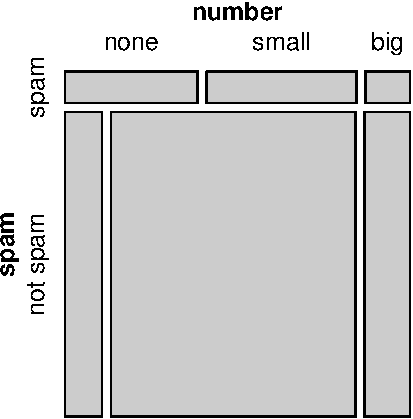
\includegraphics{06-Categorical-Data_files/figure-latex/mosaic63-fig-1.pdf}
\caption{\label{fig:mosaic63-fig}Mosaic plot with \texttt{spam} as the first variable}
\end{figure}

\hypertarget{the-only-pie-chart-you-will-see-in-this-course-hopefully}{%
\subsection{The only pie chart you will see in this course, hopefully}\label{the-only-pie-chart-you-will-see-in-this-course-hopefully}}

While pie charts are well known, they are not typically as useful as other charts in a data analysis. A \textbf{pie chart} is shown in Figure \ref{fig:pie61-fig}. It is generally more difficult to compare group sizes in a pie chart than in a bar plot, especially when categories have nearly identical counts or proportions. In the case of the \emph{none} and \emph{big} categories, the difference is so slight you may be unable to distinguish any difference in group sizes.

\begin{Shaded}
\begin{Highlighting}[]
\FunctionTok{pie}\NormalTok{(}\FunctionTok{table}\NormalTok{(email}\SpecialCharTok{$}\NormalTok{number), }\AttributeTok{col=}\NormalTok{COL[}\FunctionTok{c}\NormalTok{(}\DecValTok{3}\NormalTok{,}\DecValTok{1}\NormalTok{,}\DecValTok{2}\NormalTok{)], }\AttributeTok{radius=}\FloatTok{0.75}\NormalTok{)}
\end{Highlighting}
\end{Shaded}

\begin{figure}
\centering
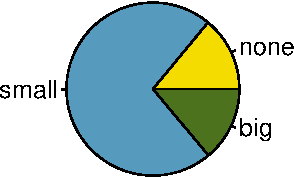
\includegraphics{06-Categorical-Data_files/figure-latex/pie61-fig-1.pdf}
\caption{\label{fig:pie61-fig}A pie chart number for the email data set.}
\end{figure}

Pie charts are popular in the Air Force due to the ease of generating them in Excel and PowerPoint. However, the values for each slice are often printed on top of the chart making the chart irrelevant. We recommend a minimum use of pie charts in your work.

\hypertarget{comparing-numerical-data-across-groups}{%
\subsection{Comparing numerical data across groups}\label{comparing-numerical-data-across-groups}}

Some of the more interesting investigations can be considered by examining numerical data across groups. This is the case where one variable is categorical and the other is numerical. The methods required here aren't really new. All that is required is to make a numerical plot for each group. Here two convenient methods are introduced: side-by-side box plots and density plots.

We will take a look again at the subset of \texttt{county\_complete} data set and compare the median household income for counties that gained population from 2000 to 2010 versus counties that had no gain. While we might like to make a causal connection here, remember that these are observational data and so such an interpretation would be unjustified.

This section will give us a chance to perform some data wrangling. We will be using the \texttt{tidyverse} verbs in the process. Data wrangling is an important part of analysis work and typically takes a significant portion of the analysis work.

Here is the code to generate the data we need.

\begin{Shaded}
\begin{Highlighting}[]
\FunctionTok{library}\NormalTok{(usdata)}
\end{Highlighting}
\end{Shaded}

\begin{Shaded}
\begin{Highlighting}[]
\NormalTok{county\_M377 }\OtherTok{\textless{}{-}}\NormalTok{ county\_complete }\SpecialCharTok{\%\textgreater{}\%} 
  \FunctionTok{select}\NormalTok{(name, state, pop2000, pop2010, }\AttributeTok{fed\_spend=}\NormalTok{fed\_spending\_2009, }\AttributeTok{poverty=}\NormalTok{poverty\_2010, }
         \AttributeTok{homeownership =}\NormalTok{ homeownership\_2010, }\AttributeTok{multi\_unit =}\NormalTok{ housing\_multi\_unit\_2010, }
         \AttributeTok{income =}\NormalTok{ per\_capita\_income\_2010, }\AttributeTok{med\_income =}\NormalTok{ median\_household\_income\_2010) }\SpecialCharTok{\%\textgreater{}\%}
  \FunctionTok{mutate}\NormalTok{(}\AttributeTok{fed\_spend=}\NormalTok{fed\_spend}\SpecialCharTok{/}\NormalTok{pop2010)}
\end{Highlighting}
\end{Shaded}

First, as a reminder, let's look at the data.

\emph{What do we want \texttt{R} to do}? We want to select the variables \texttt{pop2000}, \texttt{pop2010}, and \texttt{med\_income}.

\emph{What does \texttt{R} need}? It needs the data object, and variable names.

We will use the \texttt{select()} and \texttt{inspect()} functions.

\begin{Shaded}
\begin{Highlighting}[]
\NormalTok{county\_M377 }\SpecialCharTok{\%\textgreater{}\%}
  \FunctionTok{select}\NormalTok{(pop2000,pop2010,med\_income) }\SpecialCharTok{\%\textgreater{}\%}
  \FunctionTok{inspect}\NormalTok{()}
\end{Highlighting}
\end{Shaded}

\begin{verbatim}
## 
## quantitative variables:  
##            name   class   min       Q1 median    Q3     max     mean        sd
## ...1    pop2000 numeric    67 11223.50  24621 61775 9519338 89649.99 292547.67
## ...2    pop2010 numeric    82 11114.50  25872 66780 9818605 98262.04 312946.70
## ...3 med_income numeric 19351 36956.25  42450 49144  115574 44274.12  11547.49
##         n missing
## ...1 3139       3
## ...2 3142       0
## ...3 3142       0
\end{verbatim}

Notice that three counties are missing population values, reported as \texttt{NA}. Let's remove them and find which counties increased population by creating a new variable.

\begin{Shaded}
\begin{Highlighting}[]
\NormalTok{cc\_reduced }\OtherTok{\textless{}{-}}\NormalTok{ county\_M377 }\SpecialCharTok{\%\textgreater{}\%}
  \FunctionTok{drop\_na}\NormalTok{(pop2000) }\SpecialCharTok{\%\textgreater{}\%}
  \FunctionTok{select}\NormalTok{(pop2000,pop2010,med\_income) }\SpecialCharTok{\%\textgreater{}\%}
  \FunctionTok{mutate}\NormalTok{(}\AttributeTok{pop\_gain =} \FunctionTok{sign}\NormalTok{(pop2010}\SpecialCharTok{{-}}\NormalTok{pop2000))}
\end{Highlighting}
\end{Shaded}

\begin{Shaded}
\begin{Highlighting}[]
\FunctionTok{tally}\NormalTok{(}\SpecialCharTok{\textasciitilde{}}\NormalTok{pop\_gain,}\AttributeTok{data=}\NormalTok{cc\_reduced)}
\end{Highlighting}
\end{Shaded}

\begin{verbatim}
## pop_gain
##   -1    0    1 
## 1097    1 2041
\end{verbatim}

There were 2,041 counties where the population increased from 2000 to 2010, and there were 1,098 counties with no gain, only 1 county had a net of zero, or a loss. Let's just look at the counties with a gain or loss in side-by-side boxplot. Again, we will use \texttt{filter()} to select the two groups and then make the variable \texttt{pop\_gain} into a categorical variable, more data wrangling.

\begin{Shaded}
\begin{Highlighting}[]
\NormalTok{cc\_reduced }\OtherTok{\textless{}{-}}\NormalTok{ cc\_reduced }\SpecialCharTok{\%\textgreater{}\%}
  \FunctionTok{filter}\NormalTok{(pop\_gain }\SpecialCharTok{!=} \DecValTok{0}\NormalTok{) }\SpecialCharTok{\%\textgreater{}\%}
  \FunctionTok{mutate}\NormalTok{(}\AttributeTok{pop\_gain =} \FunctionTok{factor}\NormalTok{(pop\_gain,}\AttributeTok{levels=}\FunctionTok{c}\NormalTok{(}\SpecialCharTok{{-}}\DecValTok{1}\NormalTok{,}\DecValTok{1}\NormalTok{),}\AttributeTok{labels=}\FunctionTok{c}\NormalTok{(}\StringTok{"Loss"}\NormalTok{,}\StringTok{"Gain"}\NormalTok{)))}
\end{Highlighting}
\end{Shaded}

\begin{Shaded}
\begin{Highlighting}[]
\FunctionTok{inspect}\NormalTok{(cc\_reduced)}
\end{Highlighting}
\end{Shaded}

\begin{verbatim}
## 
## categorical variables:  
##       name  class levels    n missing
## 1 pop_gain factor      2 3138       0
##                                    distribution
## 1 Gain (65%), Loss (35%)                       
## 
## quantitative variables:  
##            name   class   min       Q1  median      Q3     max     mean
## ...1    pop2000 numeric    67 11217.25 24608.0 61783.5 9519338 89669.37
## ...2    pop2010 numeric    82 11127.00 25872.0 66972.0 9818605 98359.23
## ...3 med_income numeric 19351 36950.00 42443.5 49120.0  115574 44253.24
##             sd    n missing
## ...1 292592.28 3138       0
## ...2 313133.28 3138       0
## ...3  11528.95 3138       0
\end{verbatim}

The \textbf{side-by-side box plot} is a traditional tool for comparing across groups. An example is shown in Figure \ref{fig:sbysbox61-fig} where there are two box plots, one for each group and drawn on the same scale.

\begin{Shaded}
\begin{Highlighting}[]
\NormalTok{cc\_reduced }\SpecialCharTok{\%\textgreater{}\%}
  \FunctionTok{gf\_boxplot}\NormalTok{(med\_income}\SpecialCharTok{\textasciitilde{}}\NormalTok{pop\_gain,}
             \AttributeTok{subtitle=}\StringTok{"The income data were collected between 2006 and 2010."}\NormalTok{,}
             \AttributeTok{xlab=}\StringTok{"Population change from 2000 to 2010"}\NormalTok{,}
             \AttributeTok{ylab=}\StringTok{"Median Household Income"}\NormalTok{) }\SpecialCharTok{\%\textgreater{}\%}
  \FunctionTok{gf\_theme}\NormalTok{(}\FunctionTok{theme\_bw}\NormalTok{())}
\end{Highlighting}
\end{Shaded}

\begin{figure}
\centering
\includegraphics{06-Categorical-Data_files/figure-latex/sbysbox61-fig-1.pdf}
\caption{\label{fig:sbysbox61-fig}Side-by-side box plot for median household income, where the counties are split by whether there was a population gain or loss from 2000 to 2010.}
\end{figure}

Another useful plotting method uses \textbf{density plots} to compare numerical data across groups. A histogram bins data but is highly dependent on the number and boundary of the bins. A density plot also estimates the distribution of a numerical variable but does this by estimating the density of data points in a small window around each data point. The overall curve is the sum of this small density estimate. A density plot can be thought of as a smooth version of the histogram. Several options go into a density estimate such as the width of the window and type of smoothing function. These ideas are beyond the point here and we will just use the default options. Figure \ref{fig:dens61-fig} is a plot of the two density curves.

\begin{Shaded}
\begin{Highlighting}[]
\NormalTok{cc\_reduced }\SpecialCharTok{\%\textgreater{}\%}
  \FunctionTok{gf\_dens}\NormalTok{(}\SpecialCharTok{\textasciitilde{}}\NormalTok{med\_income,}\AttributeTok{color=}\SpecialCharTok{\textasciitilde{}}\NormalTok{pop\_gain,}\AttributeTok{lwd=}\DecValTok{1}\NormalTok{) }\SpecialCharTok{\%\textgreater{}\%}
  \FunctionTok{gf\_theme}\NormalTok{(}\FunctionTok{theme\_bw}\NormalTok{()) }\SpecialCharTok{\%\textgreater{}\%}
  \FunctionTok{gf\_labs}\NormalTok{(}\AttributeTok{x=}\StringTok{"Median household income"}\NormalTok{,}\AttributeTok{y=}\StringTok{""}\NormalTok{,}\AttributeTok{col=}\StringTok{"Population }\SpecialCharTok{\textbackslash{}n}\StringTok{Change"}\NormalTok{)}
\end{Highlighting}
\end{Shaded}

\begin{figure}
\centering
\includegraphics{06-Categorical-Data_files/figure-latex/dens61-fig-1.pdf}
\caption{\label{fig:dens61-fig}Density plots of median household income for counties with population gain versus population loss}
\end{figure}

\begin{quote}
\textbf{Exercise}:\\
Use the box plots and density plots to compare the incomes for counties across the two groups. What do you notice about the approximate center of each group? What do you notice about the variability between groups? Is the shape relatively consistent between groups? How many \emph{prominent} modes are there for each group?\footnote{Answers may vary a little. The counties with population gains tend to have higher income (median of about \$45,000) versus counties without a gain (median of about \$40,000). The variability is also slightly larger for the population gain group. This is evident in the IQR, which is about 50\% bigger in the \emph{gain} group. Both distributions show slight to moderate right skew and are unimodal. There is a secondary small bump at about \$60,000 for the \emph{no gain} group, visible in the density plot, that seems out of place. (Looking into the data set, we would find that 8 of these 15 counties are in Alaska and Texas.) The box plots indicate there are many observations far above the median in each group, though we should anticipate that many observations will fall beyond the whiskers when using such a large data set.}
\end{quote}

\begin{quote}
\textbf{Exercise}:\\
What components of each plot in Figures 8 and 9 do you find most useful?\footnote{The side-by-side box plots are especially useful for comparing centers and spreads, while the density plots are more useful for seeing distribution shape, skew, and groups of anomalies.}
\end{quote}

\hypertarget{homework-problems-5}{%
\section{Homework Problems}\label{homework-problems-5}}

Create an Rmd file for the work including headers, file creation data, and explanation of your work. Make sure your plots have a title and the axes are labeled.

\begin{enumerate}
\def\labelenumi{\arabic{enumi}.}
\tightlist
\item
  \textbf{Views on immigration}
\end{enumerate}

910 randomly sampled registered voters from Tampa, FL were asked if they thought workers who have illegally entered the US should be (i) allowed to keep their jobs and apply for US citizenship, (ii) allowed to keep their jobs as temporary guest workers but not allowed to apply for US citizenship, or (iii) lose their jobs and have to leave the country.

The data is in the \textbf{openintro} package in the \texttt{immigration} data object.

\begin{enumerate}
\def\labelenumi{\alph{enumi}.}
\tightlist
\item
  How many levels of \emph{political} are there?\\
\item
  Create a table using \texttt{tally}.
\item
  What percent of these Tampa, FL voters identify themselves as conservatives?
\item
  What percent of these Tampa, FL voters are in favor of the citizenship option?
\item
  What percent of these Tampa, FL voters identify themselves as conservatives and are in favor of the citizenship option?
\item
  What percent of these Tampa, FL voters who identify themselves as conservatives are also in favor of the citizenship option? What percent of moderates and liberal share this view?
\item
  Create a stacked bar chart.
\item
  Using your plot, do political ideology and views on immigration appear to be independent? Explain your reasoning.
\end{enumerate}

\begin{enumerate}
\def\labelenumi{\arabic{enumi}.}
\setcounter{enumi}{1}
\tightlist
\item
  \textbf{Views on the DREAM Act} The same survey from Exercise 1 also asked respondents if they support the DREAM Act, a proposed law which would provide a path to citizenship for people brought illegally to the US as children.
\end{enumerate}

The data is in the \textbf{openintro} package in the \texttt{dream} data object.

\begin{enumerate}
\def\labelenumi{\alph{enumi}.}
\tightlist
\item
  Create a \textbf{mosaic} plot.
\item
  Based on the mosaic plot, are views on the DREAM Act and political ideology independent?
\end{enumerate}

\pagebreak

\begin{enumerate}
\def\labelenumi{\arabic{enumi}.}
\setcounter{enumi}{2}
\tightlist
\item
  \textbf{Heart transplants}
\end{enumerate}

The Stanford University Heart Transplant Study was conducted to determine whether an experimental heart transplant program increased lifespan. Each patient entering the program was designated an official heart transplant candidate, meaning that he was gravely ill and would most likely benefit from a new heart. Some patients got a transplant and some did not. The variable \emph{transplant} indicates which group the patients were in; patients in the treatment group got a transplant and those in the control group did not. Another variable called \emph{survived} was used to indicate whether or not the patient was alive at the end of the study.

The data is in the \textbf{openintro} package and is called \texttt{heart\_transplant}.

\begin{enumerate}
\def\labelenumi{\alph{enumi}.}
\tightlist
\item
  Create a \textbf{mosaic} plot.
\item
  Based on the mosaic plot, is survival independent of whether or not the patient got a transplant? Explain your reasoning.
\item
  Using the variable \texttt{survtime}, create side-by-side boxplots for the control and treatment groups.
\item
  What do the box plots suggest about the efficacy (effectiveness) of transplants?
\end{enumerate}

  \bibliography{book.bib,packages.bib}

\end{document}
